\documentclass[aos]{imsart}


%% Packages
\RequirePackage{amsthm,amsmath,amsfonts,amssymb}
\RequirePackage{natbib}
%\RequirePackage[authoryear]{natbib}%% uncomment this for author-year citations
\RequirePackage[colorlinks,citecolor=blue,urlcolor=blue]{hyperref}
\RequirePackage{graphicx,xcolor}
\graphicspath{{../figures}}
%\RequirePackage{lineno} % for line numbers

\startlocaldefs
%%%%%%%%%%%%%%%%%%%%%%%%%%%%%%%%%%%%%%%%%%%%%%
%%                                          %%
%% Uncomment next line to change            %%
%% the type of equation numbering           %%
%%                                          %%
%%%%%%%%%%%%%%%%%%%%%%%%%%%%%%%%%%%%%%%%%%%%%%
%\numberwithin{equation}{section}
%%%%%%%%%%%%%%%%%%%%%%%%%%%%%%%%%%%%%%%%%%%%%%
%%                                          %%
%% For Axiom, Claim, Corollary, Hypothesis, %%
%% Lemma, Theorem, Proposition              %%
%% use \theoremstyle{plain}                 %%
%%                                          %%
%%%%%%%%%%%%%%%%%%%%%%%%%%%%%%%%%%%%%%%%%%%%%%
\theoremstyle{plain}
\newtheorem{axiom}{Axiom}
\newtheorem{claim}[axiom]{Claim}
\newtheorem{theorem}{Theorem}[section]
\newtheorem{proposition}{Proposition}
\newtheorem{lemma}[theorem]{Lemma}

%%%%%%%%%%%%%%%%%%%%%%%%%%%%%%%%%%%%%%%%%%%%%%
%%                                          %%
%% For Assumption, Definition, Example,     %%
%% Notation, Property, Remark, Fact         %%
%% use \theoremstyle{remark}                %%
%%                                          %%
%%%%%%%%%%%%%%%%%%%%%%%%%%%%%%%%%%%%%%%%%%%%%%
\theoremstyle{remark}
\newtheorem{definition}[theorem]{Definition}
\newtheorem*{example}{Example}
\newtheorem*{fact}{Fact}
\newtheorem{remark}{Remark}[section]

%%%%%%%%%%%%%%%%%%%%%%%%%%%%%%%%%%%%%%%%%%%%%%
%% Please put your definitions here:        %%
%%%%%%%%%%%%%%%%%%%%%%%%%%%%%%%%%%%%%%%%%%%%%%

\RequirePackage[utf8]{inputenc} % allow utf-8 input
\RequirePackage[T1]{fontenc}    % use 8-bit T1 fonts
\RequirePackage{multicol,booktabs,longtable}       % professional-quality tables
\RequirePackage{bm}  % blackboard math symbols
\RequirePackage{nicefrac}       % compact symbols for 1/2, etc.
\RequirePackage{microtype}      % microtypography
\RequirePackage{cleveref}       % smart cross-referencing
\RequirePackage{psfrag,epsf}
%\usepackage[authoryear]{natbib}
\RequirePackage{caption,subcaption}
\usepackage{enumitem}


%%%%%%%%%%%%%%%%%%%%%%%%%%%%%%%%%%%%%%%%%%%%%
% CUSTOM COMMANDS %
%%%%%%%%%%%%%%%%%%%%%%%%%%%%%%%%%%%%%%%%%%%%%
% Double symbol for sets
\def\E{\mathbb{E}}
\def\R{\mathbb{R}}
\def\C{\mathbb{C}}
\def\I{\mathbb{I}}
\def\Z{\mathbb{Z}}
\def\N{\mathbb{N}}

% Calligraphic
\newcommand{\Hcal}{\mathcal{H}}
\newcommand{\Rcal}{\mathcal{R}}
\newcommand{\Lcal}{\mathcal{L}}
\newcommand{\Mcal}{\mathcal{M}}
\newcommand{\Gcal}{\mathcal{G}}
\newcommand{\Fcal}{\mathcal{F}}
\newcommand{\Kcal}{\mathcal{K}}
\newcommand{\Scal}{\mathcal{S}}
\newcommand{\Tcal}{\mathcal{T}}

% Math operations
\newcommand{\ind}[1]{\boldsymbol{1}\{#1\}}
\newcommand{\abs}[1]{\left\lvert #1 \right\rvert}
\newcommand{\norm}[1]{\left\Vert #1 \right\Vert}
\newcommand{\dash}{^{\prime}}
\newcommand{\ddash}{^{\prime\prime}}
\DeclareMathOperator*{\argmin}{arg\,min}
\renewcommand{\deg}{^{\circ}}
\newcommand{\arrowf}[1]{\ensuremath{\displaystyle {\mathop {\longrightarrow}_{#1 \rightarrow \infty}\,}}}

% Matrix symbols
\newcommand{\bb}[1]{\boldsymbol{#1}}
\newcommand{\bbhat}[1]{\widehat{\boldsymbol{#1}}}
\newcommand{\tr}{^{\intercal}}
\newcommand{\trace}{\text{tr}}
\newcommand{\kernel}[1]{\bb{K}(\bb{x}, \bb{X}(#1))}


% Probability Symbols
\newcommand{\prob}{\mathbb{P}}
\newcommand{\normdist}{\mathcal{N}}
\newcommand{\cov}{\mathrm{Cov}}
\newcommand{\var}{\mathrm{Var}}
\newcommand{\multi}{\mathrm{Multinomial}}
\newcommand{\ber}{\mathrm{Bernoulli}}
\newcommand{\given}{\hspace{1pt}\vert\hspace{1pt}}
\newcommand{\conv}[1]{\ensuremath{\, \displaystyle {\mathop {\longrightarrow}^{#1}}}\, }

%%%%%%%%%%%%%%%%%%%%%%%%%%%%%%%%%%%%%%%%%%%%%%%%

% \def\X{\bm{X}}
% \def\L{\bm{L}}
% \def\Y{\bm{Y}}
% \newcommand{\w}{\mathbf{w}}
% \newcommand{\eps}{\varepsilon}
% % Caligraphic
% \def\F{\mathcal{F}}
% \def\M{\mathcal{M}}


% Begin of commands by Claudia =================
\definecolor{mygreen}{rgb}{0.09,0.62,0.45} 
\definecolor{myorange}{rgb}{0.83,0.37,0.10} % taken by Claudia - see below
\definecolor{myblue}{rgb}{0.06,0.45,0.69}  % taken by Subhrajyoty for comments and changes
\definecolor{myred}{rgb}{0.94,0.20,0.13}
\definecolor{mypurple}{RGB}{76,0,153} % taken by Claudia - see below

\newcommand{\sd}[1]{ {\color{red}{ [\textbf{SD:} {#1}] }}}
\newcommand{\srcomment}[1]{ {\color{myblue}{ [\textbf{SR:} \textit{#1} ] }}}
\newcommand{\sredit}[1]{ {\color{myblue}{#1}} }

\newcommand{\cn}[1]{ {\color{myorange}{ [\textbf{CN:} {#1} ] }}}
\newcommand{\cnam}[1]{\textcolor{mypurple}{#1}}

\newenvironment{pfofThm}{\noindent{\bf Proof of Theorem}}{\hfill $\square$ \\}
\newenvironment{pfofLem}{\noindent{\bf Proof of Lemma}}{\hfill $\square$ \\}

%------------------------------------------

\endlocaldefs

\begin{document}

\begin{frontmatter}
\title{Nonparametric quantile regression for spatio-temporal processes}
%\title{A sample article title with some additional note\thanksref{t1}}
\runtitle{Nonparametric quantile regression}
%\thankstext{T1}{A sample additional note to the title.}

\begin{aug}
%%%%%%%%%%%%%%%%%%%%%%%%%%%%%%%%%%%%%%%%%%%%%%%
%% Only one address is permitted per author. %%
%% Only division, organization and e-mail is %%
%% included in the address.                  %%
%% Additional information can be included in %%
%% the Acknowledgments section if necessary. %%
%% ORCID can be inserted by command:         %%
%% \orcid{0000-0000-0000-0000}               %%
%%%%%%%%%%%%%%%%%%%%%%%%%%%%%%%%%%%%%%%%%%%%%%%
\author[A]{\fnms{Soudeep}~\snm{Deb}\ead[label=e2]{soudeep@iimb.ac.in}\orcid{0000-0003-0567-7339}}
\author[B]{\fnms{Cl\'audia}~\snm{Neves}\ead[label=e3]{claudia.neves@kcl.ac.uk}\orcid{0000-0003-1201-5720}}
\and
\author[C]{\fnms{Subhrajyoty}~\snm{Roy}\ead[label=e1]{subhrajyoty\_r@isical.ac.in}\orcid{0000-0003-0909-5635}},

%%%%%%%%%%%%%%%%%%%%%%%%%%%%%%%%%%%%%%%%%%%%%%
%% Addresses                                %%
%%%%%%%%%%%%%%%%%%%%%%%%%%%%%%%%%%%%%%%%%%%%%%


\address[A]{Decision Sciences,
Indian Institute of Management Bangalore\printead[presep={,\ }]{e2}}

\address[B]{Department of Mathematics,
King's College London\printead[presep={,\ }]{e3}}
\end{aug}

\address[C]{Applied Statistics Division, Indian Statistical Institute Kolkata\printead[presep={,\ }]{e1}}



\begin{abstract}
%
We establish convergence rates for this nonparametric infinite-dimensional methodology relating quantile regression, investigating conditions under which it estimation is feasible and of good overall quality. We also address main computational issues faced and discussed how these were averted. Finally, we present a finite sample study the empirical performance of the proposed estimation method as well as testing procedure. \cnam{Our proposed infinite-dimensional framework for inference builds on a non-trivial combination of moment-type results borne by a functional central limit theorem tailored to martingale differences.}
%
\end{abstract}

\begin{keyword}[class=MSC]
\kwd[Primary ]{00X00}
\kwd{00X00}
\kwd[; secondary ]{00X00}
\end{keyword}

\begin{keyword}
\kwd{First keyword}
\kwd{second keyword}
\end{keyword}

\end{frontmatter}
%%%%%%%%%%%%%%%%%%%%%%%%%%%%%%%%%%%%%%%%%%%%%%
%% Please use \tableofcontents for articles %%
%% with 50 pages and more                   %%
%%%%%%%%%%%%%%%%%%%%%%%%%%%%%%%%%%%%%%%%%%%%%%
%\tableofcontents

\section{Introduction}\label{sec:introduction}

In the context of various economic or environmental research problems, it is often important to estimate the effect of a covariate on the behavior of the quantiles of a continuous response variable, and it is well known that a simple regression describing the conditional expectation of the response variable may be inadequate (see \cite{reich2012spatiotemporal} for relevant discussions). Conditional quantiles, in this regard, can provide a much better description of the spread of the conditional distribution in both tails. 

Originally proposed by \cite{koenker1978regression}, quantile regression in the simplest setting serves as an alternative approach to mean regression without requiring the strict assumption about normally distributed residuals in the linear models. In fact, conditional quantiles can provide adequate description of the data about robustness to heavy-tailed error distributions and presence of outliers, cf.\ \cite{chaudhuri1997average,ezzahrioui2008asymptotic}. Naturally, quantile estimation in time series or space-time data offers a plethora of applications in real life. Our leading example in this article is the analysis of conditional quantiles of electricity load profiles originating from smart-meter households' records. Modelling and predicting the peak-load events can help distribution network providers maintain a stable supply chain relationship at particular times of the day or week so as to ward off potential power outages \citep[][]{jacob2020forecasting}. We tackle this problem through a nonparametric approach in the setting of a multivariate time series with minimal assumptions on the data generating process. Before delving deeper into the ideology of our method, a succinct account of extant literature in this context is of the essence here. Following the aforementioned seminal paper of \cite{koenker1978regression}, various parametric, semi-parametric or nonparametric methods have been developed for conditional quantile function estimation. We particularly focus on the appeal of the nonparametric approaches which not only require minimal assumptions about the random structure and distribution of the response variable, but also enable additional flexibility in adjusting for different factors and confounding effects. 

There have been primarily two distinct nonparametric approaches towards modelling the conditional quantiles when dealing with a response variable at a time. One such approach hinges on a pinball type loss function conditional on the value of the covariate and view the resulting estimation as an optimization routine. In order to translate this into a viable and tractable problem, one often needs to restrict attention to continuous functionals of the covariate, or functionals belonging to a reproducible kernel Hilbert space \citep{takeuchi2006nonparametric}, or polynomial functions of the covariate \citep{zhou2009local}, which would typically result in smooth quantile curves. A caveat is that these methods can suffer from the undesirable quantile crossing effect, thus requiring additional constraints to be factored into the optimization setup. Contrary to that, the second approach relies on nonparametric kernel estimation of the conditional distribution function \citep[cf.][and references therein]{ferraty2005conditional,ezzahrioui2008asymptotic2}, upon which to invert for obtaining the desired conditional quantiles automatically yield conditional quantile curves that satisfy the non-crossing criterion. However, with the inversion step, the smoothness quality of the estimated quantile curve is not guaranteed and can pose a challenge in real life applications.

Turning attention to multivariate time series or spatio-temporal data, we note that despite the vastly accumulating literature on conditional quantile function estimation in the independent setting, progress in the development of feasible methodology in these domains are limited, possibly due to the challenges faced when accounting for the inherent dependencies in a meaningful way that does not break down at the laws of physics underpinning the process generating the data. To the best of our knowledge, only a few methodologies have been proposed thus far. A couple of Bayesian approaches \citep[e.g.][]{reich2011bayesian,das2017analyzing} tend to anchor on basis polynomials with ensuing considerations in terms of what makes a suitable choice for prior distributions to the relevant parameters alongside and which allowances must be brought into practice to make the method feasible. Any misspecification involving the latter is detrimental to the overall quality and feasibility of inference, thus carrying a significant potential for undermining end-users' confidence in the statistical methods being employed. Another approach \citep[e.g.][]{reich2012spatiotemporal,duan2021spatio} considers each quantile curve of different locations or coordinates separately, with the levels of quantile curves not affecting each other except for the non-crossing condition. It implies that such approaches may fail in the situations where observations at most coordinates follow a general trend (thus remaining close to the median) with only a few locations exhibiting unusual behaviour. 

In contrast to the above techniques, in this paper, we introduce a nonparametric estimator of the conditional quantile of a continuous response variable. Our method is shown to deliver smooth estimates whilst demonstrating to effectively mitigate against the above-mentioned quantile crossing effect. The extremity issue is overcome by modelling the multivariate quantiles of a distribution through an appropriate random element of the unit euclidean ball. The asymptotic properties are developed as part of the study for the proposed estimation procedure. We consider the asymptotic framework where both the number of time-points and the number of locations grow to infinity, which demand several modifications to the conventional Taylor series method used for proving consistency and asymptotic normality of estimators. Our approach leverages the sub-Gaussian properties of the data to maintain control over higher-order moments. Moreover, ensuring consistency demanded the convergence to happen in a uniform sense to account for the changing vector spaces with varying dimension, bringing additional complexity. This complexity was managed by employing concentration inequalities and a sequence of compact sets to limit the difference between estimated and true quantiles. Lastly, to address asymptotic normality, the notion needed to be appropriately modified using Portmanteau's theorem by showing that for a rich class of smooth functions with bounded derivatives, the expectation of the functional value of the normalized estimators converges to the expectation of the same functional value but applied on an appropriate slice of Gaussian process. 

The methodological details and the key results developed in this article are described in Sections \ref{Sec:MainAssump}, \ref{Sec:Estimator} and \ref{Sec:Asymptotics}. Following the asymptotic theory, we also develop simultaneous confidence bands for the spatio-temporal quantile curves across all locations and time-points in Section \ref{sec:ht}, alongside their appertaining statistical tests. In order to maintain the flow of the paper, we defer the proofs of the theoretical results until Section~\ref{sec:main-proofs}. Finally, in Section \ref{Sec:real-data}, we present the maiden real-world application of the proposed estimator to electricity load forecasting. We also include appropriate numerical investigations which offer assurances of the good overall performance of our estimator. Indeed, the key large sample properties developed in the paper are mirrored in the finite sample simulation study encompassing Appendix \ref{Sec:simulation}. 


%===================================================
\section{Spatio-temporal framework for quantile regression}
\label{Sec:MainAssump}

This paper is concerned with the statistical modeling of dependent data endowed with a spatio-temporal structure that builds on as well as expands preceding related works in \cite{de2006multivariate,zhou2010nonparametric,deb2021nonparametric}.

Let $\left\{Y(t, s):\, t \in \Tcal, s \in \Scal \right\}$ be a spatio-temporal process indexed by temporal domain consisting of a (dense) temporal horizon $\Tcal = [0, 1]$ and by a countable spatial horizon set $\Scal \subset \R^2$. Subsequently, for all $d\in \mathbb{N}$, let $\bb{X}: \Tcal \rightarrow \chi \subseteq \R^d$ be a $d$-dimensional temporal covariate process such that for each $t \in \Tcal$, $\bb{X}(t) = \left(X_1(t), \ldots, X_d(t) \right)'$ is a predictor variable in $\chi \subseteq \R^d$. In the sliding scale of generality, this covariate process can be allowed to be made fairly generic so as to encapsulate external factors that might affect the temporal dependence to the main process $Y(t, s)$, to being set out as specialized into a given periodic component aiming to capture inherent seasonality.

Out interest lies in the conditional space-time process  $Y(t, s) | \{ \bb{X}(t) : t \in \Tcal\}$ with expectation and covariance structure denoted by
\begin{equation}
      \E(Y(t, s)) = \mu(\bb{X}(t), s) \quad  \mbox{ and }  \quad
      \cov(Y(t, s_1), Y(t, s_2)) = \Sigma(\bb{X}(t), s_1, s_2),
    \label{eqn:general-setup}
\end{equation}
for every $s, s_1, s_2 \in \Scal$ and $t \in \Tcal$, bringing to the fore that the temporal dependence in the process $Y(t, s)$ is essentially driven by that of the nested covariate process $\bb{X}(t)$. Obviously, it would be beguiling to assume that $Y(t, s)$ can actually be observed in the way of covering the whole set $\Tcal \times \Scal$, so we must settle with $Y(t, s)$ indexed by the discrete subset of time points $\Tcal_n = \{t_1, t_2, \dots t_n \}$ and locations $\Scal_p = \{ s_1, s_2, \dots s_p \}$, where both $n$ and $p$ are assumed to be sufficiently large (i.e.\ both tending to $\infty$ as appropriate). This renders a more realistic framework for inference with a practical resonance: for each $t \in \Tcal_n$, consider that the data is generated by a nonparametric spatial regression model,
\begin{equation}\label{eqn:setup}
    \bb{Y}(t) = 
    \begin{pmatrix}
    Y(t,s_1)\\ Y(t, s_2) \\ \vdots \\ Y(t, s_p)
    \end{pmatrix} 
    = \bb{\mu}(\bb{X}(t)) 
    + \bb{\Sigma}^{1/2}(\bb{X}(t)) \begin{pmatrix}
   \xi_{t1}\\ \xi_{t2} \\ \vdots \\ \xi_{tp}
    \end{pmatrix},
\end{equation}
where $\bb{\mu}(\bb{X}(t))$ is a random vector in $\mathbb{R}^p$ of the form
\begin{equation*}
    \bb{\mu}(\bb{X}(t)) := \begin{pmatrix}
      \mu(\bb{X}(t), s_1)\\
      \mu(\bb{X}(t), s_2)\\
      \vdots \\
      \mu(\bb{X}(t), s_p)
    \end{pmatrix},
\end{equation*}
the covariance matrix is given by $\bb{\Sigma}(\bb{X}(t))$, whose $(i, j)$-th entry is $\Sigma(\bb{X}(t), s_i, s_j)$ for $1 \leqslant i, j\leqslant p$, and the (unobserved) errors $\left(\xi_{tj}\right)_{j=1, \dots p}$ are independent and identically distributed with mean zero, positive density on an interval containing $0$ (albeit not necessarily that of a normal distribution) and unit variance.  

The framework~\eqref{eqn:setup} lays bare that the key problem of estimating a spatial quantile at any give time $t \in \mathcal{T}$ fits well into the logic of estimating a $p$-multivariate quantile for the distribution of $\bb{Y}(t)$ centered at time-points $t_1, t_2, \hdots, t_n$. In this sense, the above framework remains quite general, so much so that it will enable existing methods for quantile regression to be employed, including in those situations where the spatio-temporal dependence structure is only implicitly defined as part of $\bb{\Sigma}(\bb{X}(t))$. If relevant information about the spatial dependency structure is available \emph{a priori}, then this can be encapsulated in $\bb{\Sigma}(\cdot)$ through a set of appropriate restrictions, either spanning the extent of a nonparametric class of models to being made fundamentally reliant on a certain postulated parametric model, in a process that echoes a familiar balancing act: the well-known robustness-efficiency trade-off. Since, in this paper, $\bb{Y}(t)$ essentially depends on the temporal domain through the covariate process $\bb{X}(t)$ (assumed predictable) the focus will be indeed on the nonparametric estimation of conditional multivariate quantiles of $\bb{Y}(t)$, given $\bb{X}(t) = \bb{x}$.

To this date, various definitions for a quantile of a multivariate distribution have been put forward, notably those drawing on convex hulls \citep{eddy1985ordering}, minimum volume sets \citep{einmahl1992generalized}, geometric generalization of spatial median \citep{chaudhuri1996geometric} and center outward quantile functions \citep{figalli2018continuity}. Amongst these, the geometric concept of a quantile in $\mathbb{R}^d$, $d \geqslant 2$, originating from \cite{chaudhuri1996geometric} and endorsed in \cite{KonenPaindaveine22}, stands out as the most amenable to our desired aim of extending the quantile regression framework of \cite{koenker1978regression} to the nonparametric spatio-temporal setting.

Central to this paper is the loss function $\Phi(\bb{u}, \bb{v}) = \norm{\bb{v}} + \langle \bb{u}, \bb{v}\rangle$, for all $\bb{u} \in B^{d-1} = \{ \bb{x} \in \R^d : \norm{\bb{x}} < 1 \}$ and the estimated quantile $\bb{v} \in \R^d$, in which setting a recognizable form of the  multivariate $\bb{u}$-quantile of a $d$-variate random vector $\bb{X}$ beckons: 
\begin{equation}\label{eqn:q-simple}
    Q(\bb{u}) := \arg\min_{\bb{q} \in \R^d} \, \E\left[ \Phi(\bb{u}, \bb{X} - \bb{q}) \right],
\end{equation}
\citep[cf.][p.397]{ChowChau19}. As desired, a choice of $\bb{u} \in B^{d-1}$ in~\eqref{eqn:q-simple} towards the boundary, i.e. $\norm{\bb{x}} \uparrow 1$, leads to a (high or low) extreme quantile, whereas fixing $\bb{u}$ near the origin yields spatially centered measurable functionals, including expectiles such as the mean vector ascribed to the $\Lcal_2$-objective function in \eqref{eqn:q-simple} or the spatial median in connection with $\Lcal_1$-norm. Since the vector $\bb{u}$ depends on the dimension $p$, i.e., the number of spatial points at play, which we allow to grow so as to attain asymptotic results, we consider $\bb{u}$ as a spatial process (measurable with respect to the Lebesgue measure on $\R^p$) satisfying
\begin{equation*}
    \int_{\Scal} \vert \bb{u}(s) \vert^2 ds \leqslant 1,
\end{equation*}
which, for every finite restriction $\Scal_p$ of $\Scal$, translates to $\bb{u}\vert_{\Scal_p} = (\bb{u}(s_1), \dots \bb{u}(s_p)) \in B^p$. In a similar vein, we now define for every $t \in \Tcal, \bb{x} \in \chi$, the $\bb{u}$-conditional spatial quantile of $\bb{Y}(t)$ given $\bb{X}(t) = \bb{x}$ as
\begin{equation}\label{eqn:parameter}
    Q(\bb{u} ,\bb{x} )\vert_{\R^p} = \arg\min_{\bb{q}\in \R^p} \, \E\left[ \Vert \bb{Y}(t) - \bb{q}\Vert +  \langle \bb{u}\vert_{\Scal_p}, \bb{Y}(t) - \bb{q} \rangle \mid \bb{X}(t) = \bb{x}\right],
\end{equation}
where $Q(\bb{u} ,\bb{x})\vert_{\R^p}$ highlights that the conditional quantile process $Q(\bb{u} ,\bb{x})$ is indexed by a $p$-dimenstional spatial domain $\Scal_p$. The set $\Scal_p$ has to be asymptotically dense in $\Scal$ as $p \rightarrow \infty$, i.e., for any $s \in \Scal$ and however small $\epsilon > 0$, we can find a point $s^\ast \in \Scal_p$ within the ball of radius $\epsilon$ centered at $s$ for sufficiently large $p$.  It is important to stress that the proposed framework prompts a significant generalization to the smoothing spline approach initially proposed in \cite{koenkeretal94}; the consideration of a temporal domain adds to a body of contemporary works in a substantive way, which to the extent of our knowledge have thus far been limited to the study of nonparametric spatial quantile regression. Our proposal is distinctive in that the criterion (loss) function presiding the M-estimation is no longer a fixed function but rather it is allowed to vary with $p$ whilst preserving many of the fundamental properties for quantile regression investigated in \cite{ChowChau19} and references therein. This is the key insight to extending the notion of a spatial (multivariate) quantile across a direction, towards the aim of tackling the spatio-temporal regression estimation problem posed in~\eqref{eqn:parameter}. The precise meaning of the latter statement will become apparent in Section~\ref{Sec:Estimator}.

One natural question about the definition of the conditional quantile process given in~\eqref{eqn:parameter} is that of whether the definition remains identifiable across choices of the set $\Scal_p$. For example, if $\Scal^\ast \subseteq \Scal$ is a superset of $\Scal_p$ for some fixed $p$, then the restriction of $Q(\bb{u}, \bb{x})\vert_{\Scal^\ast}$ to the set of points $\Scal_p$ should be same as $Q(\bb{u}, \bb{x})\vert_{\R_p}$. To see this, we consider $\Scal^\ast = \Scal_p \cup (\Scal^\ast - \Scal_p) = S_1 \cup S_2$ and correspondingly define $\bb{Y}_1(t), \bb{Y}_2(t)$ and $\bb{q}_1, \bb{q}_2$ as the restrictions of $\bb{Y}(t)$ and $\bb{q}$ respectively. Finally, we note that
\begin{multline*}
    Q(\bb{u}, \bb{x})\vert_{\Scal^\ast} = \argmin_{\bb{q}_1, \bb{q}_2} \E\left[ \sqrt{\Vert \bb{Y}_1(t) - \bb{q}_1\Vert^2 + \Vert \bb{Y}_2(t) - \bb{q}_2\Vert^2 } \right. \\
    \left. + \langle \bb{u}\vert_{S_1}, \bb{Y}_1(t) - \bb{q}_1 \rangle + \langle \bb{u}\vert_{S_2}, \bb{Y}_2(t) - \bb{q}_2 \rangle \vert \bb{X}(t) = \bb{x} \right].
\end{multline*}

It now clearly follows that optimizing with respect to $\bb{q}_1 \in \R^p$ yields a minimizer of \eqref{eqn:parameter} for any fixed value of $\bb{q}_2$, thus ensuring identifiability.

%
%===================================================
\section{Nonparametric spatio-temporal quantile estimation}
\label{Sec:Estimator}


For ease of introduction, we firstly address the case  where we look at one location at a time. This corresponds to the case of $p = 1$ in model~\eqref{eqn:setup}, whereby the canonical nonparametric quantile estimator arises as the kernel-weighted version of the quantile $q$ of order $\tau \in (0,1)$ of the corresponding empirical probability distribution function of $Y(t)$ given $\bb{X}(t) = \bb{x}$ on $\chi= \{x_1, \ldots, x_n\} \subset \R^d$. Formally, for $u\equiv u(\tau) = (2\tau - 1)$, $0 < \tau < 1$, the quantile $q$ of order $\tau$ is the minimizer of 
\begin{equation}\label{EstimatorSimple}
    \mathcal{M}_{u,n}^{(1)}(q)= \sum_{i=1}^n k(\bb{x}, \bb{X}(t_i)) \left( \vert Y(t_i) - q\vert + u \cdot (Y(t_i) - q) \right).
\end{equation}

In this respect, we note that $\mathcal{M}_{u,n}^{(1)}$ is convex on $\R$. With $\tau= 1/2$ standing for the median as the minimizer of $\mathcal{M}_{u,n}^{(1)}$, then $u$ can be viewed as a gauge for central displacement or tail-relatedness, since the greater the $\vert u\vert$ the more tail-relatable the quantile. Clearly, finding minimizers of~\eqref{EstimatorSimple} configures an $M$-estimation problem, and with the stated sample criterion function incorporating a kernel function of bandwidth $b_n$, this is one of a nonparametric nature. By this token, a generalization to the $p$-multivariate case can be readily achieved by taking matrix valued kernel functions $\bb{K}(\cdot, \cdot)$, suitably normalized, into the inner product that constitutes~\eqref{EstimatorSimple} thus giving way to the following definition of a nonparametric spatio-temporal $\bb{u}$-quantile that mirrors \eqref{eqn:parameter} in the associated sequence of statistical experiments: for $\bb{u}\vert_{\Scal_p} \in \R^p$ comprised of the set $\{ u(s): s \in \Scal_p \}$, we define the estimator
\begin{equation} \label{eqn:estimator}
    \hat{q}_n(\bb{u} ,\bb{x}) := \arg\min_{\bb{q}\in \R^p} \mathcal{M}_{\bb{u},n}^{(p)}(\bb{q}),    
\end{equation}
where 
\begin{equation}
    \mathcal{M}_{\bb{u},n}^{(p)}(\bb{q}):= \frac{1}{n} \sum_{i=1}^n  \left\{\left\Vert \bb{Y}(t_i) - \bb{q}\right\Vert_{\bb{K}(t_i)} + \left\langle\bb{u}\vert_{\Scal_p}, \bb{Y}(t_i) - \bb{q} \right\rangle_{\bb{K}(t_i)} \right\},
    \label{eqn:m-u-n}
\end{equation}
for which we write
\begin{align*}
    \bb{K}(t_i) & := \kernel{t_i}\\
    \left\Vert \bb{Y}(t) - \bb{q}\right\Vert_{\bb{K}(t)}^2 
    & := \norm{\kernel{t}(\bb{Y}(t) - \bb{q})}^2,\\
    \left\langle\bb{u}, \bb{Y}(t) - \bb{q} \right\rangle_{\bb{K}(t)} 
    & := \bb{u}\tr \kernel{t} (\bb{Y}(t) - \bb{q}).
\end{align*}

If the objective function $\mathcal{M}_{\bb{u}, n}^{(p)}$ in \eqref{eqn:m-u-n} has been highlighted to depend on both the parameter dimension $p$ and sample size $n$, in view of~\eqref{eqn:parameter} its counterpart population version (for criterion function) is laid out as
\begin{equation*}
    \mathcal{M}_{\bb{u}}^{(p)}(\bb{q}) := \E\left[ \Vert \bb{Y}(t) - \bb{q}\Vert +  \langle \bb{u}\vert_{\Scal_p}, \bb{Y}(t) - \bb{q} \rangle \mid \bb{X}(t) = \bb{x}\right].
\end{equation*}

Later on, in Section~\ref{Sec:Asymptotics}, this setting will be expanded with $p$ taken as a sequence of positive integers indexed in $n$.


%------- (A1) --- (A5) ------
%
Below, we collect the key assumptions underpinning the asymptotic results established in this paper, as well as noting that each of which will be invoked as deemed appropriate and/or necessary throughout.
%

\begin{enumerate}[label=(A\arabic*),ref=(A\arabic*)]
    \item\label{assum:predictable} The covariate process $\bb{X}(t)$ is a predictable process, i.e., there exists a sequence of random variables $\{ \epsilon_{t}: t = t_1, t_2, \dots \}$, with its natural filtration $\Fcal_{t}$ independent of the random variables $\xi_{tj}$, such that $\bb{X}(t_i)$ is $\Fcal_{t_{(i-1)}}$-measurable for any $t_i \in \Tcal_n$.
    \item\label{assum:openconvex} There exists a sequence of convex, open sets $\mathcal{U}_1 \subseteq \R, \mathcal{U}_2 \subseteq \R^2, \ldots, \mathcal{U}_p  \subseteq \R^p$ where the sequence of criterion functions $\mathcal{M}_{\bb{u},n}^{(p)}$, defined as in~\eqref{eqn:m-u-n} takes on the vector-valued $\bb{q} \in \mathcal{U}_p$, for all $t_i \in \Tcal$, and for any fixed $p \in \mathbb{N}$ not depending on $n$. Moreover, we assume that $\inf_{\bb{q} \in \mathcal{U}_p} \inf_{t_i \in \Tcal_p} \Vert \bb{Y}(t_i) - \bb{q}\Vert > \delta$ for some sufficiently small $\delta > 0$, independent of $n$ as well as of $p$.
    \item\label{assum:kernelmatrix} The kernel matrix $\kernel{t}$ is a positive definite ($p\times p$) matrix for all $t \in \Tcal$ and $\bb{x} \in \chi$, and the support of the conditional distribution of each $\bb{Y}(t_1), \dots \bb{Y}(t_n)$, provided  $\bb{X}(t) = \bb{x}$ is not enclosed in a straight line in $\mathcal{S}$~\citep[cf.][]{ChowChau19}.
\end{enumerate}


Assumption \ref{assum:predictable} on the predictable process $\bb{X}(t)$ makes it possible to write $\bb{X}(t_i) = h(\dots, \epsilon_{t_{(i-2)}}, \epsilon_{t_{(i-1)}})$ for some measurable function $h: \R^\infty \rightarrow \R^d$. It is a common assumption in related literature. Assumption \ref{assum:openconvex} is an operational assumption, which in conjunction with \ref{assum:kernelmatrix}, ensures that $\mathcal{M}_{\bb{u},n}^{(p)}$  consists of a sequence of random convex functions on $\mathcal{U}_p$, for every $p \geqslant 1$; hence it forms a sequence of continuous functions. This, in turn, ascertains the existence of M-estimators $\hat{q}_n$ in the quality of a uniquely defined sequence of minimizers of $\mathcal{M}_{\bb{u},n}^{(p)}$. Alongside these, we note that the objective function $\mathcal{M}_{\bb{u},n}^{(p)}(\bb{q})$ is strictly convex in its argument $\bb{q}$, and the same conclusion is true for $\mathcal{M}_{\bb{u}}^{(p)}(\bb{q})$ regardless of the square-integrable spatial process $\bb{u}$ such that $\int_{\Scal}\vert u(s)\vert^2 ds \leq 1$, and for every fixed $p \in \N$. This strict convexity ensures that the true quantile $\bb{q}_0$ is a well-separated minimizer of $\mathcal{M}_{\bb{u}}^{(p)}$, that is, there exists a $\bb{q}_0 \in \mathcal{U}_p$ for which $\inf_{\bb{q}: \, \Vert \bb{q} -\bb{q}_0 \Vert \geqslant \delta }\, \left(\mathcal{M}_{\bb{u}}^{(p)} (\bb{q})- \mathcal{M}_{\bb{u}}^{(p)} (\bb{q}_0) \right) >0$, for arbitrarily small $\delta > 0$, where $\delta$ may depend on $p$.



\subsection{Estimation algorithm}

The idea behind the Iteratively Re-weighted Least Squares (IRLS) type estimation as an effective means to achieve minimization in \eqref{eqn:estimator} is to replace the objective function with an equivalent version whose iterative minimization leads to the closest answer to the original problem of obtaining a quantile estimator $\hat{q}_n(\bb{u} ,\bb{x})$. Firstly, we expand the sample criterion function  $\mathcal{M}_{\bb{u},n}$ as follows:
\begin{equation*}
   \frac{1}{n}\sum_{i=1}^n \frac{\left(\bb{Y}(t_i) - \bb{q}\right)\tr \bb{K}^2(t_i) \left(\bb{Y}(t_i) - \bb{q} \right)}{\Vert \bb{Y}(t_i) - \bb{q}\Vert_{\bb{K}^2(t_i)}} + \langle \bb{u}, (\bb{Y}(t_i) - \bb{q}) \rangle_{\bb{K}(t_i)},
\end{equation*}
where we follow the convention that $\bb{y}/\Vert \bb{y} \Vert = 0$ if $ \bb{y}= \bb{0}$. In addition, we highlight that $\bb{q}$ does not change with $i$.  Henceforth, we shall use $w_i(\bb{q}) := \Vert \bb{Y}(t_i) - \bb{q}\Vert^{-1}_{\kernel{t_i}^2}$ so as to avoid notational burden. Minimization of the above with respect to $\bb{q}$ yields the sequence of estimators $\hat{q_n}$:
\begin{equation}
    \hat{\bb{q}}_n = \left\{ \frac{1}{2}\sum_{i=1}^n \bb{K}(t_i)\bb{u} + \sum_{i=1}^n w_i(\bb{q})\bb{K}^2(t_i) \bb{Y}(t_i)\right\}/{\sum_{i=1}^n w_i(\bb{q})\bb{K}^2(t_i) }.
    \label{eqn:iteration}
\end{equation}
The above \cnam{expression} suggests that, given an initial estimate $\hat{\bb{q}}^{(0)}$, it is possible to use \eqref{eqn:iteration} iteratively in order to improve estimation at the next iteration, $\bb{q}^{(k+1)}$: by calculating $w_i(\bb{q}^{(k)})$, for all $i = 1, 2, \dots n$, using the current estimate and then using \eqref{eqn:iteration} to go to the next step of the iteration. Despite the matrix $ \sum_{i=1}^n w_i(\bb{q})\bb{K}(t_i)$ is guaranteed positive definite with probability tending to one, in practice it may become numerically singular at some stage of the iteration, particularly when the number of locations $p$ is large. By adding a small positive number $\rho$ to the diagonal elements of this matrix, such a numerical blunder can be easily averted. The hyperparameter $\rho$ subsequently becomes the Lagrangian coefficient associated with a new constraint for the objective function \eqref{eqn:estimator}: $\Vert \bb{q}\Vert \leqslant C$, for some fixed $C$ positive number. Indeed, it is of straightforward verification that the IRLS scheme upon \eqref{eqn:iteration} will reduce the value of the objective function at the next iteration, i.e., $\Mcal_n(\bb{q}^{(k+1)}) \leqslant \Mcal_n(\bb{q}^{(k)})$ for all $k \in \N$. Combining this fact with the strict convexity of the objective function, it follows that the solution of the algorithm converges to the global minimizer of $\Mcal_n(\bb{q})$ since it is inherently assumed that the set of global minimizers is non-empty. 


\subsection{Choice of the kernel and associated bandwidth}\label{sec:bandwidth-choice}

The matrix-valued kernel function $\kernel{t}$ involving the bandwidth $b_n>0$ requires suitable normalizing constants $c_n>0$. Specifically, we consider the matrix
\begin{equation*}
    \kernel{t} = c_n^{-1} \Kcal\left( \dfrac{\bb{x} - \bb{X}(t)}{b_n} \right),
\end{equation*}
given in terms of a symmetric and continuous kernel $\Kcal: \R^d \rightarrow \R^{p\times p}$, with compact support on $B^{d-1} = \{ \bb{x} \in \R^d : \Vert \bb{x}\Vert \leqslant 1\}$, in keeping with the formulation we typically encounter for such nonparametric adjacency matrices of weights~\citep[see e.g.][]{deb2021nonparametric,zhao2008confidence}. Specific choices for constants $b_n, c_n >0$ must be based not only on theoretical considerations, but also be informed by empirical evidence on the behavior of competing estimators in situations of repeated sampling with varying size, all considered against the backdrop of assumptions threaded in the relevant subject literature. For example, univariate nonparametric kernel estimators for a trend in time series, which have been proposed in~\cite{zhao2008confidence}, appear suitably normalised via $c_n = \sqrt{n\,b_n}$. We also assume that $\Kcal(0) = c_n\bb{I}_p$, similar to the univariate case where the kernel function at origin is taken to be equal to $1$.


\subsection{Key properties of the nonparametric quantile estimator}
The results encompassing this section, summarized in Lemma~\ref{lemma:estimating-eqn} and ensuing considerations, are viewed as fundamental steps to establishing performance guarantees of proposed nonparametric methodology for quantile estimation. Indeed, a desirable property of a quantile estimator is affine equivariance: if the samples $\bb{Y}(t)$ are changed to $\bb{A}\bb{Y}(t) + \bb{b}$ for some non-singular matrix $\bb{A}$, the estimator should also exhibit the same affine transformation. We note that the proposed quantile estimator $\hat{q}(\bb{u} ,\bb{x})$ resulting from~\eqref{eqn:estimator} is equivariant under location transformation, i.e., employing a shift to observations through $\bb{Y}(t_i) + \bb{a}$ changes the sequence of estimators accordingly to $\hat{q}_n(\bb{u} ,\bb{x}) + \bb{a}$. Although the equivariance also holds in general with respect to a scale transformation $c\bb{Y}(t_i)$, for some scalar $c \in (0, \infty)$, verification of the orthogonal equivariance property (or more general affine equivariance property) is dependent on the incorporating kernel matrix $\bb{K}(t_i)$~\citep[see][]{chaudhuri1996geometric,Chen1996,KonenPaindaveine22}.

As \cnam{highlighted in Section~\ref{sec:introduction}, quantile estimators should generally exhibit two key properties: non-crossing of the quantiles and smoothness of the estimator as a function of the data.} In the following discussion, we demonstrate how upon a very minimal set of assumptions, both these properties follow in relation to $\widehat{\bb{q}}_n(\bb{u}, \bb{x})$.

For each $n \geqslant 1$, the quantile estimator $\hat{q}_n(\bb{u} ,\bb{x})$ is continuous with respect to observables $\bb{Y} = \left(\bb{Y}(t_1), \dots \bb{Y}(t_n)\right)$. In view of assumption~\ref{assum:openconvex}, we can without loss of generality restrict the optimization to a compact set $\mathcal{Q} \subseteq \R^p$ containing the true targeted quantile. Consequently, $\hat{q}_n(\bb{u} ,\bb{x}) = \bb{q}(\bb{Y}) = \argmin_{\bb{q} \in \mathcal{Q}} \mathcal{M}_{\bb{u},n} (\bb{q}, \bb{Y})$. Now, let $\bb{Y}_r \rightarrow \bb{Y}_0$ be a converging sequence with $r = 1, 2, \dots$, and let $\bb{q}_r = \bb{q}(\bb{Y}_r)$ for every $r \in \N$. We proceed with a subsequencing argument: for any $\{ \bb{q}_{r_k} \}_{k \in \mathbb{N}}$, the compactness of $\mathcal{Q}$ ensures that $\{ \bb{q}_{r_k} \}$ has an accumulation point $\bb{q}'$, say. Hence, we have that $\mathcal{M}_{\bb{u},n}(\bb{q}_{r_k}, \bb{Y}_{r_k}) \leqslant  \mathcal{M}_{\bb{u},n}(\bb{q}_0, \bb{Y}_{r_k}), \ r_k \in \N$. Since $ \mathcal{M}_{\bb{u},n}$ is a continuous function of $\bb{q}$ and $r_k \rightarrow \infty$, then $ \mathcal{M}_{\bb{u},n}(\bb{q}', \bb{Y}_0) \leqslant  \mathcal{M}_{\bb{u},n}(\bb{q}_0, \bb{Y}_0)$, thus entailing $\bb{q}' = \bb{q}_0$ for any subsequence, from which the continuity of the estimator ensues.

The next lemma outlines the desirable non-crossing property in any quantile estimation methodology (e.g. in line with Theorem 2.1.2 of \cite{chaudhuri1996geometric}). It is mainly a technical lemma aiming to justify that the M-estimator $\hat{q}_n(\bb{u} ,\bb{x})$, viewed as the approximate (asymptotic) solution of the convex optimization problem~\eqref{eqn:estimator}, gains the configuration of a $Z$-estimation problem for every fixed $(\bb{u} ,\bb{x})$. This is envisaged to simplify substantially the later proofs for asymptotic normality. However, because we will need to take into account the spatial dependence structure on the basis of an infinitely growing number of locations, the rate of convergence will differ from the familiar $\sqrt{n}$ for tightness mustered by predominant asymptotic theory for $Z$-estimators (see \citet{VanderVaart1998,Kosorok2008}).

\begin{lemma}\label{lemma:estimating-eqn}
    Under conditions~\ref{assum:predictable}--\ref{assum:kernelmatrix}, for every $n, p \in \N$, $\bb{x} \in \R^d$ and $\bb{u} \in B^{p-1}$, the sequence of minimizers $\widehat{\bb{q}}_n(\bb{u}, \bb{x})$ of the objective function $\Mcal_{\bb{u},n}^{(p)}$ (as in \eqref{eqn:m-u-n}) satisfies
    \begin{equation}\label{eqn:est-equation}
        \frac{1}{n} \sum_{i=1}^n \bb{K}(t_i) \left[\dfrac{\bb{K}(t_i)(\bb{Y}(t_i) - \hat{q}_n(\bb{u} ,\bb{x}))  }{ \Vert \bb{K}(t_i)(\bb{Y}(t_i) - \hat{q}_n(\bb{u} ,\bb{x})) \Vert } + \bb{u}\right] = \bb{0},
    \end{equation}
    for $\widehat{\bb{q}}_n(\bb{u}, \bb{x}) \notin \{ \bb{Y}(t_1), \dots, \bb{Y}(t_n) \}$. The true quantile $Q(\bb{u} ,\bb{x})$ in the quality of minimizer of $\Mcal_{\bb{u}}^{(p)}$ verifies the population version of \eqref{eqn:est-equation}, specifically
    \begin{equation}
        \E_{\bb{Y}(t) \mid \bb{X}(t) = \bb{x}}\left[ \dfrac{\bb{Y}(t)- Q(\bb{u} ,\bb{x}) }{\Vert \bb{Y}(t) - Q(\bb{u} ,\bb{x}) \Vert } + \bb{u}\right] = \bb{0}.
        \label{eqn:est-equation-true}
    \end{equation}
\end{lemma}

\cnam{The actionable idea stemming from Lemma~\ref{lemma:estimating-eqn} -- that we may regard \eqref{eqn:est-equation} as an estimating equation for obtaining $\hat{q}_n(\bb{u} ,\bb{x})$ from a finite sample data with $n$ time-points and $p$ spatial points -- gives rise to} an alternative Newton-Raphson type algorithm for obtaining the estimator. Notice that, for $\bb{u} = 0$, the estimating equation simply corresponds to a weighted spatial median estimate of $\bb{Y}(t_i)$ values, weighted by the covariate process $\{\bb{X}(t)\}$ through the kernel matrix \cnam{$\bb{K}(t)=\kernel{t}$}. However, for $\bb{u} \neq 0$, there is \cnam{an additional term creeping up in the way of an approximation bias, thereby increasing or decreasing the coordinates of $\hat{q}_n(x, \bb{u})$ as appropriate in a data-driven manner. This is found to play a key role to ensuring that the estimated quantile curves yielded by our methodology enjoy the non-crossing property. Further details are provided in the next section.} 


%===================================================
\section{Results}
\label{Sec:Asymptotics}

The nonparametric quantile estimator introduced in Section~\ref{Sec:Estimator} enjoys a number of  desirable  large-sample properties. This section is aimed at addressing these by allowing the \cnam{number of spatial locations $p$ tend to infinity, albeit in a controlled manner relatively to $n \rightarrow \infty$. The obtained} asymptotic properties provide the theoretical justification for the distinctive features of the quantile estimation \cnam{and ensuing testing methodology} proposed in this paper.

\cnam{We now fix some more notation in order to progress.} A bounded sequence of numbers $\{x_n\}$ is throughout written as $x_n=\mathcal{O}(1)$, springing out to the notation $x_n= \mathcal{O}(y_n)$ if $x_n/y_n= \mathcal{O}(1)$. In general, if the random sequence $X_n$ is tight, we write $\norm{X} = \mathcal{O}_p(1)$, and if $\norm{X}/\norm{Y} \conv{P} 0$ we denote this fact by $X_n= o_p(Y_n)$, as $n \rightarrow \infty$.

Let $\Tcal_n = {t_1, \dots, t_n}$ denote the set of observable time-points that satisfy the smoothing condition $\max_{2\leqslant i \leqslant n} \vert t_i - t_{i-1}\vert \rightarrow 0$ as $n \rightarrow \infty$. We also require that $\Tcal_n$ is asymptotically dense in the temporal horizon $\Tcal$. In other words, for any $\tilde{t} \in \Tcal$, there exists a sequence of points $\tilde{t}_n \in \Tcal_n$ such that $\vert \tilde{t} - \tilde{t}_n\vert \rightarrow 0$.

\begin{theorem}\label{thm:consistency}
    Assume conditions~\ref{assum:predictable}-\ref{assum:kernelmatrix} hold. \cnam{Suppose that the number of spatial locations $p$ is such that $p=p_n = o(n^{1/2})$, as $n \rightarrow \infty$.} Then, for all $\bb{x}$ lying in the compact set $\chi$, the sequence of estimators $\widehat{\bb{q}}_n(\bb{u}, \bb{x})$ of the population (theoretical) quantile $Q(\bb{u}, \bb{x})$ \cnam{satisfies}
    \begin{equation}\label{eqn:consistency}
        \Vert \widehat{\bb{q}}_n(\bb{u}, \bb{x}) - Q(\bb{u}, \bb{x}) \Vert = \mathcal{O}_p(p^2/n),
    \end{equation}
    \cnam{provided a} square-integrable spatial process $\bb{u}$, i.e.  $\int_{\Scal} \vert u(s)\vert^2 ds < 1$.
\end{theorem}

\cnam{As part of~Theorem \ref{thm:consistency}, the number of spatial locations $p$ is allowed to tend to infinity but at a vanishing rate relatively to $n^{1/2}$. The requirement that $p_n = o(n^{1/2})$, as $n\rightarrow \infty$, means in particular that the case of positive constant $p$ stays within grasp. It turns out that such a mild restriction on the growth rate of $p_n$ is indeed what it takes to ensuring the consistency of the quantile estimator established in the theorem.
For ascertaining the asymptotic normality of the proposed quantile estimator, however, the number of spatial locations must align with the initial requirement that $\Scal_p$ becomes asymptotically dense in $\Scal$.}

 Analogously to the temporal domain, we fix the setting where the observable spatial points $\Scal_p = { s_1, s_2, \dots, s_p }$ satisfy the condition $\max_{1 \leqslant j \neq k \leqslant n} d(s_j, s_k) \rightarrow 0$ as $p \rightarrow \infty$. Here, $d(s_j, s_k)$ represents the geodesic distance between the spatial coordinates $s_j$ and $s_k$. This ensures that $\Scal_p$ becomes dense in $\Scal$ with a growing number of spatial locations $p_n$ based on the geodesic metric. Also, the bandwidth $b_n$ of the kernel matrix, architected and discussed in Section~\ref{sec:bandwidth-choice} as $b_n \rightarrow 0$, must be such that and $nb_n \rightarrow \infty$ as $n \rightarrow \infty$ so that the maximum eigenvalue of $\kernel{t}$ is uniformly tight.


\subsection{Assumptions}


While assumptions~\ref{assum:predictable}-\ref{assum:kernelmatrix} in Section~\ref{Sec:Estimator} are aimed at laying the groundwork for this paper, the next set of assumptions (B1)-(B5) are required for establishing our main results appertaining  the limiting distribution for the proposed quantile estimator.

Let $f_{t}$ denote the joint probability density function of $\bb{X}(t)$ and $\Gcal_{k}$ be the $\sigma$-algebra generated by $\{ \bb{Y}(t, s), \bb{X}(t): t \leqslant t_k, s \in \Scal \}$. Additionally, let $\mathcal{P}_k$ be the projection operator defined as $\mathcal{P}_k(Z) := \E(Z\mid \Gcal_{k}) - \E(Z\mid \Gcal_{k-1})$, for all $k \in \Z$. Akin to~\cite{zhao2008confidence}, we define the cumulative effect 
\begin{equation*}
    \Xi_n  := n\Theta_{2n}^2 + \alpha_n
\end{equation*}
of the first error $\bb{\xi}_0$ in predicting the covariate process $\bb{X}(n)$, where
\begin{align*}
        \Theta_n & = \sum_{i=1}^n \sup_{x\in \chi} \Vert \mathcal{P}_0(f_t(\bb{x} \mid \Gcal_i)) \Vert + \sup_{x\in \chi} \Vert \mathcal{P}_0(f_t\dash(\bb{x} \mid \Gcal_i)) \Vert,\\
        \alpha_n & = \lim_{m \rightarrow \infty} \sum_{k = n}^{m} \left( \Theta_{n+k} - \Theta_k \right)^2.
\end{align*}

\begin{enumerate}[label=(B\arabic*),ref=(B\arabic*)]
     \item\label{assum:finite-dim} Suppose that the joint probability density function $f_{t}$ is differentiable with respect to each coordinate of $\bb{X}(t)$, for each $t \in \Tcal$. This takes care of finite-dimensional distributions of the observable process.
     \item\label{assum:bandwidth} The bandwidth $b_n>0$ satisfies the following boundary condition, as $n \rightarrow \infty$,
     \begin{equation*}
         \max \left( b_n^{4/3}\log n , \, \frac{(\log n)^3}{nb_n^3} , \frac{ (\log n)^2}{b_n^{4/3}} \frac{\Xi_n}{n^2}\right) = o(1).
    \end{equation*}
    \item\label{assum:kernelbound} There exists a constant $ c >1$ such that
    \begin{equation*}
        \dfrac{1}{c} < \sup_{t \in \Tcal} \dfrac{\lambda_1(\bb{K}(t))}{\lambda_p(\bb{K}(t))} < c,
    \end{equation*}
    \noindent where \cnam{$\bb{K}(t)= \kernel{t}$} is the $p\times p$ the kernel matrix as before and $\lambda_1(\bb{A})$ and $\lambda_p(\bb{A})$ denote  the largest and the smallest eigenvalues of the matrix $\bb{A}$, respectively.
    \item\label{assum:alpha-beta} The number of spatial points $p_n$ is such that $p_nb_n \rightarrow 0$ and $p_n^{9/8}b_n \rightarrow \infty$, as $n \rightarrow \infty$.
\end{enumerate}

Assumption~\ref{assum:finite-dim} is a natural and indeed a customary assumption that ensures smoothness of the probability density functions, allowing one to employ the standard techniques in asymptotic analysis. Assumption~\ref{assum:bandwidth} is a further restriction to the growth of the bandwidth $b_n$ of the kernel matrix, which exerts influence on the strength of dependence of the process. From~\ref{assum:bandwidth}, it results that $b_n^{-1} (n^{-1/3} \log n) = o(1)$, thus imposing a lower bound on $b_n$. Analogously, \ref{assum:bandwidth} implies that $b_n (\log n)^{3/4} = o(1)$, which provides an upper bound for $b_n$. A popular  choice for $b_n>0$ is that of the type $c_0n^{-\beta}$ for some (fixed) constant $c_0>0$; if used in tandem with the kernel proposed in Section~\ref{sec:bandwidth-choice}, then $b_n = n^{-1/5}$ is singled out  in~\citet{zhao2008confidence} for producing satisfactory results. Next, we note that the third term embedded in~\ref{assum:bandwidth},
%
\begin{equation*}
%    \frac{ (\log n)^2}{b_n^{4/3}} \frac{\Xi_n}{n^2} =
    \left( \dfrac{\log n}{n^{1/3} b_n} \right)^2 \left( nb_n \right)^{2/3} \frac{\Xi_n}{n^2}.
\end{equation*}
%
implies that  $\Xi_n/n^{2} = o(1)$ due to the earlier condition $b_n^{-1} (n^{-1/3} \log n) = o(1)$ in conjunction with $nb_n \rightarrow \infty$. Because each summand of the partial $\Theta_n$ gives the contribution of $\epsilon_0$ (as in~\ref{assum:predictable}) to the associated predictor $\bb{X}(t_{i+1})$, this term plays a relevant role in moderating the dependence of $X(t)$. In particular, the random vectors $\bb{X}(t_{i})$ must satisfy a summability property designed to maintain the integrity of the predictor process $\bb{X}(t)$ by way of ensuring that the covariance structure of the spatio-temporal process is well-defined and can always be estimated. On the whole, this assumption~\ref{assum:predictable} has a number of parallels with published works on inference for spatio-temporal processes (see e.g.~\cite{zhao2008confidence,zhou2009local,deb2021nonparametric}). According to \cite{zhao2008confidence}, a condition such as this  corrals virtually  the full spectrum for the strength of dependence, from the boundary case of the predictor process $\bb{X}(t)$ exhibiting  only short-range dependence (SRD) (determined by $\lim_{n \rightarrow \infty} \Xi_n < \infty$) to a weakening long-range dependence (LRD). Assumption~\ref{assum:kernelbound} is required in order to control random oscillations of the kernel matrix. In keeping with the random matrix theory, Wigner's law asserts that the eigenvalues of the $p \times p$ covariance matrix $\bb{\Sigma}(X(t))$ are of order $\sqrt{p}$~\citep{vershynin2010introduction} for sufficiently large $p$, hence monotonically increasing with $n$ and $p$. This means that for any fixed $t \in \Tcal$, the ratio of the largest and the smallest eigenvalue of $\bb{K}(t)$ remains bounded for sufficiently large $p$. For the first finitely many terms, boundedness of this ratio is ensured by tightness and positive definiteness of the kernel matrix $\bb{K}(t)$. Assumption~\ref{assum:kernelbound} is a stronger version of this statement that requires uniform boundedness over all choices of $t \in \Tcal$. This assumption guarantees that there exists a suitable kernel matrix such that eigenvalues of the covariance matrices of the kernel-weighted observables $\bb{Y}(t)$ remain bounded. Finally, assumption~\ref{assum:alpha-beta} in conjunction with the bounds on bandwidth $b_n$ that ensue from \ref{assum:bandwidth} implies that $ 
   (\log n)^{-2/3} \ll  p_n \ll  \left( n/\log n\right)^{1/3}$.



\subsection{Asymptotic distribution}

In this section, we establish the gaussian limting distribution attained by the proposed quantile estimator.  The consistency of the proposed quantile estimator expounded \cnam{in Theorem~\ref{thm:consistency} and accompanying text herald} the rate at which the number of locations $p$ can grow \cnam{in relation} to the number of time-points $n$ so as to make this nonparametric quantile estimation feasible. 

%In order to proceed to obtaining the asymptotic distribution of the quantile estimator, we need some more notation and one proposition, which we are going to introduce next. 

\cnam{Continuing along the lines of \eqref{eqn:m-u-n} and  adding to the notation introduced as part of Lemma~\ref{lemma:estimating-eqn},} we define
\begin{equation*}
    \nabla \Mcal_{\bb{u},n}^{(p)} (\bb{q}) := -\dfrac{1}{n}\sum_{i=1}^n \bb{K}(t_i) \left[ \dfrac{\bb{K}(t_i) (\bb{Y}(t_i) - \bb{q})}{\Vert \bb{Y}(t_i) - \bb{q} \Vert_{\bb{K}(t_i)}} + \bb{u} \right]\label{eqn:m-u-n-prime}.
\end{equation*}
Let $\nabla^2 \Mcal_{\bb{u},n}^{(p)} (\bb{q}_0)$ be the matrix whose $i$-th row \cnam{is comprised of} the gradient of $\nabla \Mcal_{\bb{u},n}^{(p)} (\bb{q})$ with respect to the $i$-th coordinate of $\bb{q}$. Also, let us denote by $\nabla^3 \Mcal_{\bb{u},n}^{(p)}(\bb{q})$ the third order tensor whose $(i,j,k)$-th entry is the third order derivative of $\Mcal_{\bb{u},n}^{(p)}(\bb{q})$ with respect to the $i,j$ and $k$-th coordinate of $\bb{q}$. \cnam{We have the following proposition.}


\begin{proposition}\label{prop:P1P3}
Under assumptions~\ref{assum:predictable}-\ref{assum:kernelmatrix} and~\ref{assum:finite-dim}-\ref{assum:alpha-beta}, the following hold:
\begin{enumerate}[label=(P\arabic*),ref=(P\arabic*)]
    \item\label{prop:first-div-dist} There exists a $p$-variate Gaussian random variable $\bb{Z}(\bb{q}_0)$ with mean parameter $\eta_t(\bb{q}_0)$ and dispersion matrix $\Omega_t(\bb{q}_0)$, such that 
    \begin{equation*}
        \sup_{\Vert \bb{u}\Vert \leq 1}\sup_{f \in \mathcal{F}} \left\Vert \E\left[ f\left( (pb_n)^{-1} \nabla \Mcal_{\bb{u},n}^{(p)} (\bb{q}_0) \right) \right] - \E\left[ f(\bb{Z}(\bb{q}_0) \right] \right\Vert = \mathcal{O}(p^2/n)
    \end{equation*}
     \noindent with probability tending to $1$, where $\mathcal{F}$ is the set of bounded thrice differentiable functions from $\R^{p}$ to $\R$ with a bounded derivative \cnam{up to the third order.}
    \item\label{prop:second-div-mat} There exists a collection of positive definite matrices $\{ \Psi_t(\bb{q}_0) \}$ for all possible $\bb{q}_0 \in \mathcal{Q}_p$ as a minimizer of \eqref{eqn:parameter} with respect to the spatial points $\Scal_p$, such that 
    \begin{equation*}
        \sup_{\bb{q}_0 \in \mathcal{Q}_p} \left\Vert \nabla^2 \Mcal_{\bb{u},n}^{(p)}(\bb{q}_0)-\Psi_t(\bb{q}_0) \right\Vert \xrightarrow{P} 0.
    \end{equation*}
    \item\label{prop:third-div-bound} There exists $M > 0$ (not depending on $n$) such that 
    \begin{equation*}
       \sup_{\bb{q} \in \mathcal{Q}_p} \left\Vert \nabla^{3} (\Mcal_{\bb{u},n}^{(p)})(\bb{q}) \right\Vert \leq M.
    \end{equation*}
\end{enumerate}
    
\end{proposition}

The three parts~\ref{prop:first-div-dist}-\ref{prop:third-div-bound} embodying Proposition~\ref{prop:P1P3}, whose proof is deferred to Appendix~\ref{appA},  mirror each of the \cnam{usual} necessary steps to demonstrating the asymptotic normality of $M$-estimators~\citep[cf.][]{huber2011robust}. The asymptotic development for the proposed estimator of the conditional quantile of $\bb{Y}$, given that $\bb{X}(t) = \bb{x}$ for any fixed $t \in \Tcal$,\cnam{stays within this remit.} Although general in their principle, the innovation in \cnam{Proposition~\ref{prop:first-div-dist} is that it amplifies complementary works on quantile regression by enabling the increasing dimension $p=p_n \rightarrow \infty$, as $n \rightarrow \infty$. The simpler i.i.d. version analogous to this proposition} can be traced back to \cite{portnoy1986clt}, and contemporary related results accommodating a changing $p_n$ can be found in~\cite{das2020clt}. Our infinite-dimensional framework shall build on a combination of (pre-asymptotic) moment-type results approached by a functional central limit theorem for martingale differences~\citep[cf.][]{belloni2018high}.


In order to lessen the notational burden throughout the remainder of this paper, we \cnam{employ the substitutions outlined in the following:}
\begin{align}
    \bb{\eta}(t_i) = \E\left[ \bb{K}(t_i)(\bb{Y}(t_i) - \bb{q}_0) \mid \Gcal_{t_i-} \right] & = \bb{K}(t_i)\left( \bb{\mu}(t_i) - \bb{q}_0 \right),\label{eqn:notation-eta}\\
    \bb{V}_1(t_i) = \var\left[ \bb{K}(t_i)(\bb{Y}(t_i) - \bb{q}_0) \mid \Gcal_{t_i-} \right] & = \bb{K}(t_i) \bb{\Sigma}(t_i) \bb{K}(t_i),\label{eqn:notation-v1}\\
    \bb{V}_2(t_i) = \left( \dfrac{1}{\Vert \bb{\eta}(t_i) \Vert}\bb{I}_p - \dfrac{\bb{\eta}(t_i)\bb{\eta}(t_i)\tr}{\Vert \bb{\eta}(t_i)\Vert^3} \right),\label{eqn:notation-v2}
\end{align}
where $\bb{I}_p$ denotes the identity matrix of order $p$.


With the key quantities \cnam{ $\bb{\eta}_t(\bb{q}), \bb{\Omega}_t(\bb{q})$ and $\bb{\Psi}_t(\bb{q})$, encapsulating the mean and covariance that characterizes the dependence structure of the finite-dimensional distributions associated with the limiting gaussian process for the proposed quantile estimation, namely}
\begin{align}
    \bb{\eta}_t(\bb{q}_0) := & \dfrac{1}{npb_n}\sum_{i=1}^n \bb{K}(t_i) \left[ \dfrac{\bb{\mu}(t) - \bb{q}_0}{\Vert \bb{\mu}(t) - \bb{q}_0 \Vert} - \dfrac{\bb{\eta}(t_i)}{\Vert \bb{\eta}(t_i) \Vert} \right]\label{eqn:keydef-eta}\\
    \bb{\Omega}_t(\bb{q}_0) := & \dfrac{1}{n^2p^2b_n^2} \sum_{i=1}^n \bb{K}(t_i) \bb{V}_2(t_i)\bb{V}_1(t_i)\bb{V}_2(t_i)\tr \bb{K}(t_i)\label{eqn:keydef-omega}\\
    \bb{\Psi}_t(\bb{q}_0) := & \dfrac{1}{n}\sum_{i=1}^n \bb{K}(t_i) \bb{V}_2(t_i) \bb{K}(t_i)\label{eqn:keydef-psi},
\end{align}
we arrive at the main result in this paper, stated in the following theorem.

\begin{theorem}\label{thm:normal-dist}
    Define $\bb{q}_0: = Q(\bb{u}, \bb{x})$. \cnam{Under} the assumptions~\ref{assum:predictable}-\ref{assum:kernelmatrix} and~\ref{assum:finite-dim}-\ref{assum:alpha-beta}, with $\mathcal{F}$ from~\ref{prop:first-div-dist}, it holds that
    \begin{equation*}
        \sup_{\Vert \bb{u} \Vert < 1} \sup_{f \in \mathcal{F}} \left\Vert \E\left(f \left((pb_n)^{-1} (\widehat{q}_n(\bb{u},\bb{x}) - \bb{q}_0 \right)\right) - \E\left( f\left( -\bb{\Psi}_t(\bb{q}_0)^{-1}\bb{Z}(\bb{q}_0) \right) \right) \right\Vert \xrightarrow{P} 0 
    \end{equation*}
    \noindent as $n \rightarrow \infty$, where  $\bb{Z}(\bb{q}_0)$ is a $p$-variate Gaussian random vector with mean vector $\bb{\eta}_t(\bb{q}_0)$ and dispersion matrix $\bb{\Omega}_t(\bb{q}_0)$.
\end{theorem}

At this point, we tactically turn focus to sketching a proof for Proposition~\ref{prop:P1P3} since this forms the basis for the proof of Theorem~\ref{thm:normal-dist}. For the first part in reference, we start by noting that the challenge in obtaining the asymptotic distribution of $(pb_n)^{-1} \nabla\Mcal_{\bb{u},n}^{(p)}(\bb{q}_0)$ stems from \cnam{the non-linearity of the normalized term
%
$
   \bigl(  \bb{K}(t_i)(\bb{Y}(t_i) - \bb{q}_0)\bigr) / \Vert \bb{K}(t_i)(\bb{Y}(t_i) - \bb{q}_0) \Vert
$
%
with respect to \cnam{the random variables $\bb{Y}(t_i)$. A standard trick to thwart this issue is to employ a suitable Taylor's expansion for obtaining} a sufficiently sharp approximation to a linear functional of  $\bb{Y}(t_i)$ or $\bb{\xi}(t_i)$. Indeed, both expressions \eqref{eqn:notation-eta}-\eqref{eqn:notation-v2} have already been carved out in such a way as to become amenable to such an expansion: writing $\bb{K}(t_i)(\bb{Y}(t_i) - \bb{q}_0) = \bb{\eta}(t_i) + \bb{V}_1^{1/2}(t_i)\bb{\xi}(t_i)$, application of Taylor's expansion on the errors $\xi_{tj}$ thus precipitates the development}
\begin{equation*}
    \dfrac{\bb{K}(t_i)(\bb{Y}(t_i) - \bb{q}_0)}{\Vert \bb{K}(t_i)(\bb{Y}(t_i) - \bb{q}_0) \Vert} = \dfrac{\bb{\eta}(t_i)}{\Vert \bb{\eta}(t_i) \Vert} + \bb{V}_2(t_i)\bb{V}_1^{1/2}(t_i) \bb{\xi}(t_i) + O\left(\dfrac{\Vert \bb{V}_1^{1/2}(t_i)\Vert}{\Vert \bb{\eta}(t_i)\Vert^3} \Vert \bb{\xi}(t_i) \Vert^2\right),
\end{equation*}
i.e.,
\begin{multline*}
    \nabla \Mcal_{\bb{u},n}^{(p)}(\bb{q}_0)
    = \dfrac{1}{n} \sum_{i=1}^n \bb{K}(t_i) \left( \dfrac{\bb{\eta}(t_i)}{\Vert \bb{\eta}(t_i) \Vert} + \bb{u} \right) + \dfrac{1}{n} \sum_{i=1}^n \bb{K}(t_i) \bb{V}_2(t_i)\bb{V}_1^{1/2}(t_i) \bb{\xi}(t_i)\\
    + \dfrac{1}{n}\sum_{i=1}^n \mathcal{O}(\Vert \bb{K}(t_i) \Vert \Vert \bb{\eta}(t_i)\Vert^{-3} \Vert \bb{V}_1^{1/2}(t_i) \Vert \Vert \bb{\xi}(t_i) \Vert^2).
\end{multline*}
The proof now follows in three steps. Owing to Lemma~\ref{lemma:estimating-eqn}, the first term can be shown to converge to a constant which constitutes the bias. Next, application of a bespoke central limit theorem for the multidimensional martingale provided by~\citet{belloni2018high}, ensures that the asymptotic weak limit to the second term is a gaussian random variable with mean zero. Finally, \cnam{by assumption~\ref{assum:alpha-beta}, the third term vanishes to zero at the rate $\mathcal{O}(\max\{ p^{-9/4}b_n^{-2}, p^{-3/2}b_n^{-1} \})$.  Further details underpinning this proof for Proposition~\ref{prop:first-div-dist} can be found in Appendix~\ref{proof:first-div-dist}.}

\cnam{Proposition~\ref{prop:second-div-mat}, whose detailed proof is deferred to Appendix~\ref{proof:second-div-mat}, is outline as follows: by computing the second order derivative of the objective function $\Mcal_{\bb{u},n}^{(p)}(\bb{q})$, we find that
\begin{multline*}
    \nabla^2 \Mcal_{\bb{u},n}^{(p)}(\bb{q}) 
    = \dfrac{1}{n}\sum_{i=1}^n \bb{K}(t_i) \biggl[ \dfrac{I_p}{\left\Vert  \bb{Y}(t_i) - \bb{q} \right\Vert_{\bb{K}(t_i)} } 
\\ - \dfrac{\bb{K}(t_i)(\bb{Y}(t_i) - \bb{q})(\bb{Y}(t_i) - \bb{q})\tr \bb{K}(t_i)}{\left\Vert  \bb{Y}(t_i) - \bb{q} \right\Vert^3_{\bb{K}(t_i)}} \biggr] \bb{K}(t_i).
\end{multline*}
Upon splitting the above expression into a sum of martingale difference terms and a remainder term, the former (i.e. sum) normalized appropriately, can be shown to converge to zero via application of a martingale central limit theorem~\citep[see][]{belloni2018high}. The dominant component in the remainder term  boils down to $\bb{\Psi}_t(\bb{q}_0)$ with everything else being asymptotically negligible. This is achieved through a suitable Taylor's expansion.}

Finally, \cnam{regarding Proposition~\ref{prop:third-div-bound}, we find it convenient and useful} to prove the stronger statement that $\nabla^2 \Mcal_{\bb{u},n}^{(p)}(\bb{q})$ is Lipschitz with a Lipschitz constant $M$ independent of $n$ and $p$.  Starting with assumption~\ref{assum:openconvex}, we note that since $\mathcal{Q}_p$ is a compact subset of $\mathcal{U}_p$, $\Vert \bb{Y}(t_i) - \bb{q} \Vert_{\bb{K}(t_i)} \geq \lambda_p(\bb{K}(t_i)) \delta$ for all $\bb{q} \in \mathcal{Q}_p$, where $\lambda_p(\bb{A})$ is the smallest eigenvalue of the matrix $\bb{A}$. Since the kernel matrix is positive definite and has bounded entries,  it readily follows that $\nabla^2 \Mcal_{\bb{u},n}^{(p)}(\bb{q})$ is a Lipschitz function of $\bb{q}$ with a Lipschitz constant $\left(\delta^{-1} \sup_{t_i \in \Tcal_p} \lambda_1(\bb{K}(t_i))/\lambda_p(\bb{K}(t_i))\right)^{-3}$ where $\lambda_1(\bb{A})$ is the largest eigenvalue of the matrix $\bb{A}$. By assumption~\ref{assum:kernelbound}, this quantity remains bounded.




%====== Section Statistics ====================
\section{Statistical inference: interval estimation and hypotheses testing}\label{sec:ht}

While the estimation of quantile curves yielding from \eqref{eqn:estimator} possesses several desirable qualities, including the consistency and asymptotic normality, the underpinning convergence is pointwise in the temporal domain, that is, it is obtained for each value of the covariate process $\{\bb{X}(t) = \bb{x}\}$. From the practical stance, an interesting approach resides in obtaining simultaneous confidence band. Inevitably, this will require extending the asymptotic properties of the estimator to the entire temporal domain, uniformly on the index range of $\bb{X}(\cdot)$. The means to achieve this has a number of parallels with the techniques exploited in \cite{zhao2008confidence}.

To this end, we shall consider a set of values for the covariates, sufficiently apart in order that at every time-point $t$, the kernel estimator is affected by at most one of the values in that set. This is to ensure that no correlation between estimates are at play for sufficiently distant time-points. Upon the already obtained asymptotic normality results, this consideration opens way to making uniform statistical inference possible: asymptotic behavior of the proposed nonparametric estimator's sequence across multiple time-points, uniformly, is now within reach. The ultimate aim is to devise meaningful asymptotic results pertaining to partial maxima of this sequence of estimators by drawing on extreme value theory.

We define $\chi_n = \{ \bb{X}(t): t \in \Tcal_n \} \subseteq \chi$ as the range of the covariate process $\{\bb{X}(t)\}$. We assume that, for any $\bb{x}, \bb{x}\dash \in \chi_n$, $\Vert \bb{x} - \bb{x}\dash\Vert > 2b_n\rightarrow 0$ thus implying that $\chi_n$ becomes dense within $\chi$ as $n$ tends to infinity. The cardinality of  $\chi_n$ is encapsulated in $m_n$.


\subsection{Simultaneous confidence bounds} 

For the sake of simplicity, the results comprising in this section refrain to $\bb{u}$-quantiles with $\bb{u} = (2\tau - 1)\bb{1}/\sqrt{p}$ for some $\tau \in (0,1)$. This framework essentially renders quantiles that spread evenly among the considered spatial locations. We shall denote the corresponding quantile estimator by $\hat{q}_n(\tau, \bb{x})$ (or sometimes simply by $\hat{q}(\tau, \bb{x})$) whereas the true targeted quantile is denoted by $Q(\tau, \bb{x})$. In spite of this slight restriction to the framework for inference, all results derived in this section can be adapted to incorporate the more general multivariate case as before, in a relatively straightforward manner.

By construction, it follows from the definition of $\chi_n$ that, for any two points $\bb{x}_{i_1}, \bb{x}_{i_2} \in \chi_n$, $i_1 \neq i_2$, and every $\delta>0$, the exists $n_0 \in \mathbb{N}$ such that $\norm{\bb{x}_{i_1} - \bb{x}_{i_2}} < 2\delta$, $i_1, \, i_2 > n_0$. Hence, for every $t \in \Tcal_n$, $\Vert \bb{X}(t) - \bb{x}_{j}\Vert < \delta$, $j=i_1, i_2$, which results from the triangle inequality. Since $\Kcal$ has bounded support in the unit hypersphere $B^d$, it thus follows that the cross products of the weights intervening in the objective function resolve to zero, i.e.
\begin{equation}\label{eqn:nullcrossproduct}
    \bb{K}(\bb{X}(t), \bb{x}_{i_1}) \bb{K}(\bb{X}(t), \bb{x}_{i_2}) = c_n^{-2} \Kcal\left( \dfrac{\bb{X}(t)-\bb{x}_{i_1}}{b_n} \right) \Kcal\left( \dfrac{\bb{X}(t)-\bb{x}_{i_2}}{b_n} \right) = 0
\end{equation}
(the reader may wish to recall the discussion on $c_n$ as part of Section~\ref{sec:bandwidth-choice}). Equation \eqref{eqn:nullcrossproduct} lays bare that fixing two quantile levels $\tau$ and $\tau\dash$ ($0 < \tau, \tau\dash < 1$), so that objective function if optimised for $\hat{q}(\tau, \bb{x}_{i_1})$ contains the terms with weights $\bb{K}(\bb{X}(t), \bb{x}_{i_1})$ for some $t \in \Tcal_n$, whereas for the sequence of estimators $\hat{q}(\tau\dash, \bb{x}_{i_2})$ these weights amount to $\bb{K}(\bb{X}(t), \bb{x}_{i_2})$, results in the two objective functions (both for $\hat{q}(\tau, \bb{x}_{i_1})$ and $\hat{q}(\tau\dash, \bb{x}_{i_2})$) being uncorrelated, thus implying that the estimators $\hat{q}(\tau, \bb{x}_{i_1})$ and $\hat{q}(\tau\dash, \bb{x}_{i_2})$ are also uncorrelated.


\cn{Please check whether the above makes sense to you. Thanks!} \\

Therefore, by taking a multitude of points on the set $\chi_n = \{ \bb{x}_{i_1}, \bb{x}_{i_2}, \dots \bb{x}_{i_{m_n}} \}$, we obtain from Theorem~\ref{thm:normal-dist} that the estimator $\hat{q}_n(\bb{x}, \tau)(s)$ becomes asymptotically a Gaussian process on both temporal and spatial domains, for every $\bb{x} \in \chi_n$ and $s \in \Scal$. More concretely, on the finite set of spatial points $S_d = \{s_1, s_2, \dots s_d\}$ and with unit vector $\bb{l} \in \R^d$, we have for every $\bb{x} \in \chi_n$, as $n \rightarrow \infty$, that
\begin{equation}
   R_n(\bb{x}, \bb{l}, S_d) =(p b_n )^{-1} \dfrac{\bb{l}\tr (\hat{q}_n(\tau, \bb{x})\vert_{S_d} - Q(\tau, \bb{x})\vert_{S_d} - \bb{\mu}_q(\bb{x})\vert_{S_d} ) }{ \sqrt{\bb{l}\tr \bb{\Sigma}_q(\bb{x})\vert_{S_d} \bb{l} }} \xrightarrow{d} \normdist(0, 1).
\end{equation}

\noindent We highlight that $\hat{q}_n(\bb{x}, \tau)\vert_{S_d}$ and $ Q(\bb{x}, \tau)\vert_{S_d}$ respectively denote $\hat{q}_n(\bb{x}, \tau)$ and $Q(\bb{x}, \tau)$ restricted to the spatial locations in $S_d$. Letting $q_0 = Q(\tau, \bb{x})$, then $\bb{\mu}_q(x)\vert_{S_d}$ and $\bb{\Sigma}_q(x)\vert_{S_d}$ respectively denote mean and covariance structure, evaluated at the spatial locations in the set $S_d$, of the Gaussian process $\{ G(\bb{x}, s) : \bb{x} \in \chi, s \in \Scal \}$ characterized by
\begin{equation}
	\begin{split}
	\E\left[ G(\bb{x}, s) \right] & = \bb{\Psi}_{\bb{X}(t) = \bb{x}}^{-1}(\bb{q}_0) \bb{\eta}_{\bb{X}(t) = \bb{x}}(\bb{q}_0) \\
	\text{Cov}\left( G(\bb{x}, s), G(\bb{x}', s) \right) & = \begin{cases}
        \bb{\Psi}_{\bb{X}(t) = \bb{x}}^{-1}(\bb{q}_0) \bb{\Omega}_{\bb{X}(t) = \bb{x}}(\bb{q}_0) \bb{\Psi}_{\bb{X}(t) = \bb{x}}^{-1} (\bb{q}_0), & \bb{x} = \bb{x}'; \\
        0, & \bb{x} \neq \bb{x}'.
    \end{cases}
	\end{split}
\end{equation}
\noindent where the quantities $\bb{\eta}(\bb{q}_0), \bb{\Omega}(\bb{q}_0)$ and $\bb{\Psi}(\bb{q}_0)$ are as defined in~\eqref{eqn:keydef-eta}-\eqref{eqn:keydef-psi}.

\cnam{We now progress to obtaining the asymptotic behaviour of the supremum} of $G(\bb{x}, s)$ over the temporal index through $\sup_{x\in \chi_n} \hat{q}_n(\tau, \bb{x})(s)$ for any $s \in \Scal$.  From the case in point that $\hat{q}_n(\tau, \bb{x}_{i_1})$ and $\hat{q}_n(\tau\dash, \bb{x}_{i_2})$ are asymptotically uncorrelated, the next step is to apply %Theorem 5 of~\cite{zhao2008confidence}
the extreme value theorem upon the  univariate martingale difference sequence $R_n(\bb{x}_{i_k}, \bb{l}, S_d)$, $k = 0, 1, \dots,m_{n} - 1$. Owing to the rich theory of extreme values, there exist normalizing functions $ C_t$ specific to the folded normal distribution, i.e.
\begin{equation}
    C_t(z) := \frac{1}{\sqrt{2\log t}}  \left( z -  \frac{\log \log t  + \log(4 \pi)}{2} \right)
    \label{eqn:NormingBn}
\end{equation}
\citep[see][p.72]{Resnick1987}, such that the weak convergence to the Gumbel distribution function is attained in the following sense: for all $z \in \mathbb{R}$,
\begin{equation}
    \ \lim_{n\rightarrow \infty} \prob\left( \sup_{x \in \chi_{m_{n}}} \vert R_n(\bb{x}, \bb{l}, S_d) \vert \leq C_{m_{n}}(z + 2 \log m_{n} ) \right)  = \exp\{  -e^{-z}\}.
    \label{eqn:conf-1}
\end{equation}
%i.e.,
%\begin{equation*}
%    \lim_{n\rightarrow \infty} \prob\left( \sup_{x \in \chi_{m(n)} R_n^2(\bb{x}, \bb{l}, S_d) <  B^2_{m_n}(z) \right) = e^{-2e^{-z}}.
%\end{equation*}

Next, we consider the maximum eigenvalue of the matrix $\bb{M}$, denoted as $\lambda_1(\bb{M})$, for establishing the identification
\begin{equation*}
    \sup_{\norm{\bb{l}} = 1} \dfrac{\bb{l}\tr \bb{A}\bb{l}}{\bb{l}\tr \bb{B}\bb{l}} =  \lambda_1 \left(\bb{B}^{-1/2}\bb{A}\bb{B}^{-1/2} \right),
\end{equation*}
where $\bb{A}$ and $\bb{B}$ are positive definite matrices. In conjunction with the limiting distribution statement in~\eqref{eqn:conf-1}, we subsequently find that
\begin{multline}
    \lim_{n\rightarrow \infty} \prob\biggl( \sup_{\bb{x} \in \chi_{m_{n}}} \dfrac{1}{pb_n}\lambda_1\left[\bb{\Sigma}_q(\bb{x})^{-1/2}\vert_{S_d} \bb{e}(\bb{x})\vert_{S_d}\, \bb{e}(\bb{x})\vert_{S_d}\tr \bb{\Sigma}_q(\bb{x})^{-1/2}\vert_{S_d} \right] \\ < C_{m_n}(z) + \sqrt{2 \log m_{n}}\biggr) = \exp\{  -e^{-z}\},
    \label{eqn:conf-2}
\end{multline}
by taking supremum over all possible unit vectors $\bb{l}$ and whereby $\bb{e}(\bb{x})\vert_{S_d} = (\hat{q}_n(\tau, \bb{x})\vert_{S_d} - Q(\tau, \bb{x})\vert_{S_d} - \bb{\mu}_q(\bb{x})\vert_{S_d} )$. Hence, under the \cnam{assumptions~\ref{assum:predictable}-\ref{assum:kernelmatrix} and~\ref{assum:finite-dim}-\ref{assum:alpha-beta}, with a judicious choice of $\chi_{m(n)}$, i.e., so long as $\log m_n = o \left(  (p b_n )^{-2}\right)$ is satisfied,
the sequence of estimators $\hat{q}_n(\tau, \bb{x})$ can be guaranteed to fulfill} \eqref{eqn:conf-1} and~\eqref{eqn:conf-2} on a finite set of spatial locations $S_d = \{ s_1, s_2, \dots s_d \}$ from the ``larger'' set $\Scal$. This result, which is along the lines of that in Theorem 2 of~\cite{zhao2008confidence}, serves as basis to introducing simultaneous confidence bands for the $\tau$-quantile curves $Q(\tau, \bb{x})$ ascribed to multiple values $x \in \chi_n$. Because $\chi_n$ becomes increasingly dense in $\chi$ as $n$ tends to $\infty$, an asymptotic confidence band for the quantile curve $\{Q(\tau, \bb{x}): \bb{x} \in \chi\}$ naturally arises from \eqref{eqn:conf-1}.

Indeed, a contrast-like linear combination of the quantile curves across different locations stems from \eqref{eqn:conf-1} as follows: with a proper specification of the set $S_d$ and vector $\bb{l} \in \R^d$ so that $\bb{l}\tr Q(\bb{x}, \tau)$ becomes the desired contrast-like quantile curve, we find that the asymptotic simultaneous $100(1-\alpha^*)\%$-confidence bounds for $\bb{l}\tr Q(\bb{x}, \tau)\vert_{S_d}$ consist of
\begin{multline*}
    \bb{l}\tr \hat{q}_n(\bb{x}, \tau)\vert_{S_d} - \bb{l}\tr\widehat{\bb{\mu}}_q(x)\vert_{S_d} \\
    \pm \left[ C_{m_n}\left(-\log\left(-\log(1-\alpha^*/2\right))\right) + \sqrt{2 \log m_n} \right] (pb_n) \left( \bb{l}\tr \widehat{\bb{\Sigma}}_q(x)\vert_{S_d} \bb{l} \right)^{1/2},
\end{multline*}
with embedded consistent estimators $\widehat{\bb{\mu}}_q(x)$ and $\widehat{\bb{\Sigma}}_q(x)$ for the bias term $\bb{\mu}_q(x)$ and covariance $\bb{\Sigma}_q(x)$, respectively. We note that the symmetry in the confidence interval is justified by the same limiting extreme value distribution of $\inf_{\bb{x}}R_n$ and $-\sup_{\bb{x}}\abs{R_n}$, a remark that will prove useful to constructing one-sided hypothesis testing procedures.

\subsection{Two tests}

The statement in \eqref{eqn:conf-2} \cnam{can be adapted to the purpose of hypothesis testing, namely in order to} validate structural assumptions on the quantile curves across all locations simultaneously. For instance, given a null hypothesis about the structural restriction of the quantile curve $Q(\tau, \bb{x})$ at some specific quantile $\tau \in [0, 1]$, we can calculate the observed value of the test statistic
\begin{equation}\label{eqn:errors}
    \bb{e}_0(\bb{x})\vert_{\Scal_p} = (\hat{q}_n(\tau, \bb{x})\vert_{\Scal_p} - \hat{q}_0(\tau, \bb{x})\vert_{\Scal_p} - \bb{\mu}_q(x)\vert_{\Scal_p} )
\end{equation}
where $\hat{q}_0(\tau, \bb{x})$ stands the estimate of $Q(\tau, \bb{x})$ under the postulated null hypothesis $H_0$ regarding a stable regime. Then, the null hypothesis is rejected if \eqref{eqn:errors} exhibits large oscillation, i.e., at the nominal level of the test $\alpha^*$, $H_0$ is rejected if
\begin{equation*}
    \dfrac{1}{pb_n}\sup_{\bb{x} \in \chi_n} \lambda_1\left( \widehat{\bb{\Sigma}}_q(\bb{x})^{-1/2}\vert_{\Scal_p} \bb{e}_0(\bb{x})\vert_{\Scal_p}\bb{e}_0(\bb{x})\vert_{\Scal_p}\tr \widehat{\bb{\Sigma}}_q(\bb{x})^{-1/2}\vert_{\Scal_p} \right)
\end{equation*}
exceeds the critical value $c_{\alpha^*}=C_{m_n}\left(-\log\left(-\log(1-\alpha^*)\right)\right) + \sqrt{2 \log m_n}$. \cnam{Henceforth, we define $\bb{u}_{\tau} := (2\tau-1) \bb{1}_p/\sqrt{p}$.}

\cnam{A structural assumption that is often put to testing is that of homogeneity of the covariate effect across the spatial domain, which if true, automatically narrows down the spatio-temporal structure of the data to a temporal one. This is statistically parlayed in the null hypothesis $H_0^{(1)}:\, Q(\tau, \bb{x}) = \beta(\bb{x}) \bb{u}_{\tau}$, for all $\tau \in [0, 1]$. Under $H_0^{(1)}$, the estimator $\widehat{\beta}(\bb{x})$ arises from~\eqref{eqn:est-equation} as solution of:}
\begin{equation*}
    \sum_{i=1}^n \kernel{t_i} \left[\dfrac{\kernel{t_i}(\bb{Y}(t_i) - \widehat{\beta}(\bb{x})\bb{u}_{\tau} )  }{ \Vert \kernel{t_i}(\bb{Y}(t_i) - \widehat{\beta}(x)\bb{u}_{\tau} ) \Vert } + \bb{u}_{\tau}\right] = 0,
\end{equation*}
and the null hypothesis is rejected for large values of the test statistic, i.e.,
\begin{equation*}
    \dfrac{1}{pb_n} \sup_{\bb{x} \in \chi_n} \lambda_1\left( \widehat{\bb{\Sigma}}_q(\bb{x})^{-1/2}\vert_{\Scal_p} \bb{e}_1(\bb{x})\vert_{\Scal_p}\bb{e}_1(\bb{x})\vert_{\Scal_p}\tr \widehat{\bb{\Sigma}}_q(\bb{x})^{-1/2}\vert_{\Scal_p} \right) > c_{\alpha^*}\, , 
\end{equation*}
on the relevant set $\Scal_p$ of spatial locations, where
$
    \bb{e}_1(\bb{x})\vert_{\Scal_p} = (\hat{q}_n(\bb{u} ,\bb{x}_{\tau})\vert_{\Scal_p} - \widehat{\beta}(x) \bb{u}_{\tau} - \widehat{\bb{\mu}}_q(x)\vert_{\Scal_p} )
$ can be defined.

\cnam{The second testing procedure with practical importance under the realm of \eqref{eqn:setup} ascribes time to a covariate, i.e. $\bb{X}(t) = t$. The hypothesis of homogeneity over time then translates into $H_0^{(2)}:\, Q(\bb{u}_{\tau}, t)/  Q( \bb{u}_{\tau}, 1) = t$, for all $t \in (0, 1]$ and $\tau \in [0, 1]$.} At the significance level $\alpha^*$, $H_0^{(2)}$ is rejected if
\begin{equation*}
    \dfrac{1}{pb_n} \sup_{t \in (0, 1]} \lambda_1\left( \widehat{\bb{\Sigma}}_q(t)^{-1/2}\vert_{\Scal_p} \bb{e}_2(t)\vert_{\Scal_p}\bb{e}_2(t)\vert_{\Scal_p}\tr \widehat{\bb{\Sigma}}_q(t)^{-1/2}\vert_{\Scal_p} \right) > c_{\alpha^*}\, , 
\end{equation*}
with associated $ \bb{e}_2(t)\vert_{\Scal_p} = (\hat{q}_n(\bb{u}_{\tau}, t)\vert_{\Scal_p} - t\hat{q}_n(\bb{u}_{\tau}, 1)\vert_{\Scal_p}  - \widehat{\bb{\mu}}_q(x)\vert_{\Scal_p} )$.



%===================================================

\section{Proofs}\label{sec:main-proofs}

\cnam{This section contains the proofs of the key theorems in this paper as well as of their ancillary results. We begin by addressing Lemma~\ref{lemma:estimating-eqn}, which consolidates the estimating equation for the proposed nonparametric quantile estimator.}

\medskip
%\subsection{Proof of Lemma}
 
\begin{pfofLem}~\ref{lemma:estimating-eqn}:
    \cnam{Under assumption~\ref{assum:kernelmatrix}, $\bb{K}(t) = \kernel{t}$ is a positive definite matrix for any $t \in \Tcal$. Hence, $\Phi_K(\bb{u}, \bb{Y}(t) - \bb{q}) = \Vert \bb{Y}(t) - \bb{q}\Vert_{\bb{K}(t)} + \langle \bb{u}, \bb{Y}(t) - \bb{q}\rangle_{\bb{K}(t)}$ is a strictly convex function of $\bb{q}$.} Since $\widehat{\bb{q}} = \widehat{\bb{q}}_n(\bb{u}, \bb{x})$ is the minimizer of $\Mcal_{\bb{u},n}^{(p)}(\bb{q}) = \frac{1}{n}\sum_{i=1}^n \Phi_K(\bb{u}, \bb{Y}(t_i) - \bb{q})$, then for every $\bb{h} \in \R^d$,

\begin{align*}
    & \lim_{\epsilon \downarrow 0} \dfrac{1}{n\epsilon}\sum_{i=1}^n \left[ \Phi_K(\bb{u}, \bb{Y}(t_i) - \widehat{\bb{q}} + \epsilon \bb{h}) - \Phi_K(\bb{u}, \bb{Y}(t_i) - \widehat{\bb{q}} ) \right] \geqslant 0\\
    \implies & \dfrac{1}{n}\sum_{i=1}^n \lim_{\epsilon \downarrow 0} \dfrac{\Vert \bb{Y}(t_i) - \widehat{\bb{q}} + \epsilon \bb{h} \Vert_{\bb{K}(t_i)} - \Vert \bb{Y}(t_i) - \widehat{\bb{q}} \Vert_{\bb{K}(t_i)} }{ \epsilon } + \lim_{\epsilon \downarrow 0} \dfrac{ \langle \bb{u}, \epsilon \bb{h} \rangle_{\bb{K}(t_i)} }{\epsilon} \geqslant 0\\
    \implies & \dfrac{1}{n}\sum_{i=1}^{n} \left[ \dfrac{\langle \bb{Y}(t_i) - \widehat{\bb{q}}, h\rangle_{\bb{K}(t_i)} }{ \Vert \bb{Y}(t_i) - \widehat{\bb{q}} \Vert_{\bb{K}(t_i)} } + \langle \bb{u}, \bb{h}\rangle_{\bb{K}(t_i)} \right] \geqslant 0.
\end{align*}
\cnam{Using the same steps with $(-\bb{h})$ in place of $\bb{h}$ we arrive \eqref{eqn:est-equation}. Similarly, \eqref{eqn:est-equation-true} stems from \eqref{eqn:parameter}.}
\end{pfofLem}

%\subsection{Proof of Theorem~\ref{thm:consistency}}

\begin{pfofThm}~\ref{thm:consistency}:
    Defining $\bbhat{q} =\widehat{\bb{q}}_n(\bb{u}, \bb{x})$ and $\bb{q}_0 = Q(\bb{u},\bb{x})$, we write the chain of inequalities:
    \begin{align*}
        \Mcal_{\bb{u}}^{(p)}(\bbhat{q}) - \Mcal_{\bb{u}}^{(p)}(\bb{q}_0)
        & \leq \Mcal_{\bb{u}}^{(p)}(\bbhat{q}) - \Mcal_{\bb{u}}^{(p)}(\bb{q}_0) - \Mcal_{\bb{u},n}^{(p)}(\bbhat{q}) + \Mcal_{\bb{u},n}^{(p)}(\bb{q}_0)\\
        & \leq 2 \sup_{\bb{q} \in \mathcal{Q}_p} \vert \Mcal_{\bb{u}, n}^{(p)}(\bb{q}) - \Mcal_{\bb{u}}^{(p)}(\bb{q}) \vert\,,
    \end{align*}
%    \srcomment{Here is the detailed explanation of the steps: Since, $\bb{q}_0$ is the true value minimizing $\Mcal_{\bb{u}}^{(p)}$, the quantity $\Mcal_{\bb{u}}^{(p)}(\bbhat{q}) - \Mcal_{\bb{u}}^{(p)}(\bb{q}_0)$ is nonnegative, there is no additional requirement to take absolute value. Next, as $\bbhat{q}$ is the minimizer of $\Mcal_{\bb{u},n}^{(p)}$, we simply add the positive quantity $\Mcal_{\bb{u},n}^{(p)}(\bb{q}_0) - \Mcal_{\bb{u},n}^{(p)}(\bbhat{q})$ to the term on the left hand side. Finally, the supremum follows from rearranging these terms and using triangle inequality.} \cn{You're spot on! Sorry I lost track of what we're doing in here.}
     where $\mathcal{Q}_p \subseteq \R^p$ is a set containing both $\bb{q}_0$ and the sequence of estimators $\bbhat{q}_n(\bb{u}, \bb{x})$, thus enabling
    \begin{eqnarray}
    \nonumber  &     & \prob\left( \Vert \bbhat{q} - \bb{q}_0 \Vert > A p^2/n \right)\\
    \nonumber  \; &\leq & \prob\left( \Vert \bbhat{q} - \bb{q}_0 \Vert > A p^2/n, \,\Mcal_{\bb{u}}^{(p)}(\bbhat{q}) - \Mcal_{\bb{u}}^{(p)}(\bb{q}_0) < Bp^2/n \right)\\
    \nonumber   &   & \mbox{\hspace{4.5cm}} + \prob\left( \Mcal_{\bb{u}}^{(p)}(\bbhat{q}) - \Mcal_{\bb{u}}^{(p)}(\bb{q}_0) \geq Bp^2/n \right)\\
    \label{eqn:aux1}           &\leq & \prob\Bigl( \Vert \bbhat{q} - \bb{q}_0 \Vert > A p^2/n, \,\Mcal_{\bb{u}}^{(p)}(\bbhat{q}) - \Mcal_{\bb{u}}^{(p)}(\bb{q}_0) < Bp^2/n \Bigr)\\
     \label{eqn:aux2}  &    & \mbox{\hspace{4.5cm}} + \prob\biggl( \sup_{\bb{q} \in \mathcal{Q}_p} \vert \Mcal_{\bb{u}, n}^{(p)}(\bb{q}) - \Mcal_{\bb{u}}^{(p)}(\bb{q}) \vert   \geq Bp^2/2n \biggr).
    \end{eqnarray}
   
    %    =&  \prob\left( \Vert \bbhat{q} - \bb{q}_0 \Vert > A p^2/n, \, \Mcal_{\bb{u}}^{(p)}(\bbhat{q}) - \Mcal_{\bb{u}}^{(p)}(\bb{q}_0) < Bp^2/n \right) \\
    %    & \mbox{\hspace{5.8cm}} + \prob\left( \Vert \bbhat{q} - \bb{q}_0 \Vert > A p^2/n,\, \Mcal_{\bb{u}}^{(p)}(\bbhat{q}) - \Mcal_{\bb{u}}^{(p)}(\bb{q}_0) \geq Bp^2/n \right)\\
   
   
    Owing to the convexity lemma by~\citet{Pollard1991}, the objective function $\mathcal{M}_{\bb{u}}$ as part of~\eqref{eqn:parameter} is convex on \sredit{$\mathcal{Q}_p$}. Consequently, the sequence of conditional regression-quantile estimators $\hat{q}_n$ along $\bb{u}$ is well-defined and the true quantile $q_0$ is a well-separated minimizer of $\mathcal{M}_{\bb{u}}$, that is, there exists a $q_0 \in \mathcal{U}_p$ for which $\inf_{\bb{q}: \, \Vert \bb{q} -\bb{q}_0 \Vert \geqslant \delta }\, \left(\mathcal{M}_{\bb{u}} (\bb{q})- \mathcal{M}_{\bb{u}} (\bb{q}_0) \right) >0$, for arbitrarily small $\delta>0$. This ensures the boundedness of the first term in the above sum. Through application of the triangle inequality in conjunction with the Cauchy-Schwartz inequality, we obtain:
    \begin{equation*}
        \Mcal_{\bb{u}}^{(p)}(\bb{q}) \geq \Vert \bbhat{q} - \bb{q}_0\Vert (1 - \Vert \bb{u}\vert_{\Scal_p} \Vert),
    \end{equation*}
   which implies in turn that
    \begin{equation*}
        \prob\left( \Vert \bbhat{q} - \bb{q}_0 \Vert > A p^2/n, \,\Mcal_{\bb{u}}^{(p)}(\bbhat{q}) - \Mcal_{\bb{u}}^{(p)}(\bb{q}_0) < Bp^2/n \right)
        \leq \prob\left( \Vert \bb{u}\vert_{\Scal_p} \Vert > 1 - B/A \right).
    \end{equation*}
 If $\Vert \bb{u}\Vert < 1$, i.e., if not addressing an extreme quantile or the case of bounded support, it is possible to fix $B = A\epsilon$ with arbitrarily small $\epsilon > 0$, so as to ensure that $\Vert \bb{u}\vert_{\Scal_p} \Vert \leq (1-\epsilon)$, \cnam{in which case the above upper bound becomes 0. This takes care of \eqref{eqn:aux1}. }
  %  \begin{align*}
  %      & \prob\left( \Vert \bbhat{q} - \bb{q}_0 \Vert > A p^2/n \right)\\
 %       \leq & \prob\left( \Vert \bb{u}\vert_{\Scal_p} \Vert > 1 - B/A \right)
 %       + \prob\left(\, \sup_{\bb{q} \in \R^p} \Vert \Mcal_{\bb{u}, n}^{(p)}(\bb{q}) - \Mcal_{\bb{u}}^{(p)}(\bb{q}) \Vert   \geq Bp^2/2n \right).
 %   \end{align*}
    %
    Consequently, the gist of the proof is in verifying the \cnam{uniform convergence of uniform convergence embedded in \eqref{eqn:aux2}}. This is done as follows. From the subgaussian property of $\bb{Y}(t)$ together with the law of large numbers, it results that 
    \begin{equation}
        \left\vert \Mcal_{\bb{u},n}^{(p)}(\bb{q}) - \E\left[ \Vert \bb{Y}(t) - \bb{q} \Vert_{\bb{K}(t)} + \langle \bb{u}, \bb{Y}(t) - \bb{q} \rangle_{\bb{K}(t)} \right] \right\vert = \mathcal{O}_p(\sqrt{p/n})
        \label{eqn:step-mcaln-mcalkern}
    \end{equation}
  In order to connect the weighted expectation affecting the kernel $\bb{K}(t)$ with $\Mcal_{\bb{u}}^{(p)}(\bb{q})$, we invoke the law of iterated expectations upon the conditioning random variable $R = \left\Vert \bb{X}(t) - \bb{x} \right\Vert$: 
    \begin{equation*}
        \E\left[ \Vert \bb{Y}(t) - \bb{q} \Vert_{\bb{K}(t)} + \langle \bb{u}, \bb{Y}(t) - \bb{q} \rangle_{\bb{K}(t)} \right]
        = \E\left[ \E\left[ \Vert \bb{Y}(t) - \bb{q} \Vert_{\bb{K}(t)} + \langle \bb{u}, \bb{Y}(t) - \bb{q} \rangle_{\bb{K}(t)} \mid R \right] \right].
    \end{equation*}
\cnam{There is a one-to-one mapping between $R$ and the continuous measurable functional that is the kernel $\bb{K}(t)$. In particular, the event $R = 0$, amounts to $\bb{K}(t) = \bb{I}_p$ due to $\Kcal(0) = c_n\bb{I}_p$. Whence, there exists $\delta_R > 0$ such that for every $R < \delta_R$, all eigenvalues of the matrix $(\bb{K}(t) - \bb{I}_p)$ are bounded by $\sqrt{p/n}$, rendering valid the chain of inequalities:}
    \begin{align*}
        & \sredit{\left\vert \E\left[ \Vert \bb{Y}(t) - \bb{q} \Vert_{\bb{K}(t)} + \langle \bb{u}, \bb{Y}(t) - \bb{q} \rangle_{\bb{K}(t)} \right] - \E\left[ \Vert \bb{Y}(t) - \bb{q} \Vert + \langle \bb{u}, \bb{Y}(t) - \bb{q} \rangle \mid \bb{X}(t) = \bb{x} \right] \right\vert}\\
        = & \left\vert \E\left[ \E\left[ \Vert \bb{Y}(t) - \bb{q} \Vert_{\bb{K}(t)} + \langle \bb{u}, \bb{Y}(t) - \bb{q} \rangle_{\bb{K}(t)} \mid R \right] \right] - \E\left[ \Vert \bb{Y}(t) - \bb{q} \Vert + \langle \bb{u}, \bb{Y}(t) - \bb{q} \rangle \mid R = 0 \right] \right\vert \\
        = & \left\vert  \E\left[ \Vert \bb{Y}(t) - \bb{q} \Vert_{\bb{K}(t)} + \langle \bb{u}, \bb{Y}(t) - \bb{q} \rangle_{\bb{K}(t)} \mid R \leq \delta_R \right]\prob(R \leq \delta_R) \right. \\
        & \qquad \left. + \E\left[ \Vert \bb{Y}(t) - \bb{q} \Vert_{\bb{K}(t)} + \langle \bb{u}, \bb{Y}(t) - \bb{q} \rangle_{\bb{K}(t)} \mid R > \delta_R \right]\prob(R > \delta_R) \right. \\
        & \qquad \left. - \E\left[ \Vert \bb{Y}(t) - \bb{q} \Vert + \langle \bb{u}, \bb{Y}(t) - \bb{q} \rangle \mid R = 0 \right] \right\vert \\
        \leq & \left\vert \E\left[ \Vert \bb{Y}(t) - \bb{q} \Vert_{\bb{K}(t)} - \Vert \bb{Y}(t) - \bb{q} \Vert \mid R \leq \delta_R \right] \right\vert + \left\vert \E\left[ \langle \bb{u}, \bb{Y}(t) - \bb{q} \rangle_{\bb{K}(t)} - \langle \bb{u}, \bb{Y}(t) - \bb{q} \rangle \mid R \leq \delta_R \right] \right\vert \\
        & \qquad \left\vert \E\left[ \Vert \bb{Y}(t) - \bb{q} \Vert_{\bb{K}(t)} + \langle \bb{u}, \bb{Y}(t) - \bb{q} \rangle_{\bb{K}(t)} \mid R > \delta_R \right] \right\vert
    \end{align*}
    \noindent The first term can be bounded by the product of the absolute value of the maximum eigenvalue of $(\bb{K}(t) - \bb{I}_p)$ and the norm of $\Vert \bb{Y}(t) - \bb{q}\Vert$. When $R \leq \delta_R$, combining with the subgaussian behaviour of $\bb{Y}(t)$, the first term can be bounded by $\mathcal{O}(p/\sqrt{n})$. For the second term, an application of the Cauchy-Schwartz inequality combined with the fact that $\Vert \bb{u}\Vert \leq 1$ yields that it is also bounded by $\mathcal{O}(p/\sqrt{n})$. For the third term, note that as the bandwidth $b_n \rightarrow 0$, for sufficiently large $n$, $\delta_R > b_n$. Since the kernel $\Kcal$ has bounded support in the unit hypersphere $B^{d}$, it follows that $\bb{K}(t)$ can be made equal to $\bb{0}$ in the third term. Therefore,
    \begin{equation*}
        \left\vert  \E\left[ \Vert \bb{Y}(t) - \bb{q} \Vert_{\bb{K}(t)} + \langle \bb{u}, \bb{Y}(t) - \bb{q} \rangle_{\bb{K}(t)}  \right]- \Mcal_{\bb{u}}^{(p)}(\bb{q}) \right\vert = o(p/\sqrt{n}) = o(p^2/n)
    \end{equation*}
    \cn{Please check (and then indicate) which of the above $\mathcal{O}$-terms is a small o}\srcomment{Modified accordingly.}
    \noindent Combining this with~\eqref{eqn:step-mcaln-mcalkern}, we obtain that for each fixed $\bb{q} \in \R^p$, 
    \begin{equation*}
        \Vert \Mcal_{\bb{u}, n}^{(p)}(\bb{q}) - \Mcal_{\bb{u}}^{(p)}(\bb{q}) \Vert = \mathcal{O}_p(p^2/n)
    \end{equation*} 

    \sredit{The uniform convergence now follows if we can show that $\mathcal{Q}_p$ is a compact set. Thus, it is enough to show that the sequence of estimators $\bb{q}_n$ minimizing the sequence of objective functions $\Mcal_{\bb{u}, n}^{(p)}(\bb{q})$ are uniformly bounded. Without the loss of generality, consider that $0$ belongs to the convex hull of the datapoints $\{ \bb{Y}(t_i) : i = 1, 2, \dots n\}$, otherwise we can translate all datapoints suitably. By applying the sub-gaussian property of $\bb{Y}(t_i)$ and union bound, it follows that there exists some $c > 0$ such that
    \begin{equation*}
        \prob\left( \sup_{1 \leq i \leq n} \Vert \bb{Y}(t_i)\Vert > M \right) \leq ne^{-cp}.
    \end{equation*}
    \noindent By choosing sufficiently large $p = O(\log n)$, we can now make $\Mcal_{\bb{u}, n}^{(p)}(\bb{0}) < M$ with probability arbitrarily close to $1$, by bounding each $\bb{Y}(t_i)$. Also, since $\Vert \bb{u}\Vert < 1$, there exists a $\delta \in (0, 1)$ such that $\Vert \bb{u}\Vert < (1-\delta)$, and a vector $\bb{v}$ such that $\Vert \bb{v}\Vert > 2M\delta^{-1}$. Consider the objective function at a point $\bb{Y}(t_j) + \bb{v}$ for any $j = 1, 2, \dots n$;
    \begin{align*}
        \Mcal_{\bb{u}, n}^{(p)}(\bb{Y}(t_j) + \bb{v}) 
        & = \dfrac{1}{n} \sum_{i=1}^n \left[ \Vert \bb{Y}(t_i) - \bb{Y}(t_j) - \bb{v} \Vert_{\Kcal(t_i)} + \langle \bb{u}, \bb{Y}(t_i) - \bb{Y}(t_j) - \bb{v}  \rangle_{\Kcal(t_i)} \right]\\
        & \geq \Vert \bb{v}\Vert/2 - (1 - \delta)\Vert \bb{v}\Vert/2, \text{ by an application of Cauchy-Schwartz inequality}\\
        & \geq M \geq \Mcal_{\bb{u}, n}^{(p)}(\bb{0})
    \end{align*}
    By general positioning of these vectors, $\{ \bb{Y}(t_j) + \bb{v}, \bb{Y}(t_j) - \bb{v} : j = 1, \dots n\}$ do not lie in a subspace with a dimension strictly less than $p$. Combining this with the convex nature of the objective function $\Mcal_{\bb{u}, n}^{(p)}(\bb{q})$, it follows that along the boundary of the convex hull of these points also, the value of the objective function is more than $M$. Using continuity of the objective function, we find that there is a $(p-1)$-dimensional hypersphere, independent of the choice of $n$, containing the origin $0$ such that the $\Mcal_{\bb{u}, n}^{(p)}(\bb{q}) > \Mcal_{\bb{u}, n}^{(p)}(\bb{0})$ for any $\bb{q}$ lying on the boundary of that hypersphere for any $n$. Now it follows from the strict convexity of each $\Mcal_{\bb{u}, n}^{(p)}(\bb{q})$ that they have a local minimum within that hypersphere. Choosing the $\bbhat{q}_n$ as those local minima establishes the boundedness of them.     }
\end{pfofThm}

%\subsection{Proof of Theorem~\ref{thm:normal-dist}}

\begin{pfofThm}~\ref{thm:normal-dist}:
 We start by assuming that the Propostions~\ref{prop:first-div-dist}-\ref{prop:third-div-bound} hold.

    Consider a Taylor series expansion of $\nabla \Mcal_{\bb{u}, n}^{(p)}(\bb{q})$ about the true parameter $\bb{q}_0 := Q(\bb{u}, \bb{x})$ and evaluate at $\widehat{\bb{q}} := \widehat{\bb{q}}_n(\bb{u},\bb{x})$,
    \begin{align*}
        0 & = \nabla \Mcal_{\bb{u}, n}^{(p)}(\widehat{\bb{q}})\\
        & = \nabla \Mcal_{\bb{u}, n}^{(p)}(\bb{q}_0) + \nabla^2 \Mcal_{\bb{u}, n}^{(p)}(\bb{q}_0)(\widehat{\bb{q}} - \bb{q}_0) + \mathcal{O}(\Vert \widehat{\bb{q}} - \bb{q}_0\Vert^2 \left\Vert \nabla^3\Mcal_{\bb{u}, n}^{(p)}(\bb{q}) \right\Vert )
    \end{align*}
    Denoting $\nabla^{i} \Mcal_{\bb{u}, n}^{(p)}(\bb{q}_0) = \Delta_{i}$, we obtain that
    \begin{equation*}
        a_n\left( \widehat{\bb{q}} - \bb{q}_0 \right) = -a_n \Delta_{2}^{-1} \Delta_1 + \mathcal{O}(\Vert \Delta_2^{-1}\Vert p^4/n) 
    \end{equation*}
    \noindent where we use the consistency result of $\widehat{\bb{q}}$ along with proposition~\ref{prop:third-div-bound} to bound $\Vert \Delta_3\Vert$. By proposition~\ref{prop:second-div-mat}, it follows that for sufficiently large $n$,
    \begin{equation*}
        \left\Vert \Delta_2^{-1} - \bb{\Psi}(\bb{q}_0)^{-1}\right\Vert \leq \dfrac{2}{\Vert \bb{\Psi}(\bb{q}_0) \Vert^2} \left\Vert \bb{\Psi}(\bb{q}_0) - \Delta_{2}\right\Vert \leq \dfrac{Cp^2}{n\Vert \bb{\Psi}(\bb{q}_0) \Vert^2}
    \end{equation*}
    Therefore,
    \begin{align*}
        & \quad \left\vert \E\left( f\left( a_n\left( \widehat{\bb{q}} - \bb{q}_0 \right) \right) \right) - \E\left( f\left( \bb{\Psi}^{-1}(\bb{q}_0) Z(\bb{q}_0) \right)  \right) \right\vert \\
        \leq & \quad \left\vert \E\left( f\left( -a_n \Delta_{2}^{-1} \Delta_1 + \mathcal{O}(\Vert \Delta_2^{-1}\Vert p^4/n) \right) \right) - \E\left( f\left( \bb{\Psi}^{-1}(\bb{q}_0) Z(\bb{q}_0) \right)  \right) \right\vert \\
        \leq & \quad \left\vert \E\left( f\left( -a_n \Delta_{2}^{-1} \Delta_1 + \mathcal{O}(\Vert \Delta_2^{-1}\Vert p^4/n) \right) \right) - \E\left( f\left( -a_n\bb{\Psi}^{-1}(\bb{q}_0) \Delta_1 \right)  \right) \right\vert + \\
        & \qquad \qquad \left\vert \E\left( f\left( -a_n\bb{\Psi}^{-1}(\bb{q}_0) \Delta_1 \right) \right) - \E\left( f\left( \bb{\Psi}^{-1}(\bb{q}_0) Z(\bb{q}_0) \right)  \right) \right\vert\\
        \leq & \quad \E\left( \left\Vert f\dash(\widetilde{\bb{q}}) \right\Vert \left( \mathcal{O}(\Vert \Delta_2^{-1}\Vert p^4/n) + \vert a_n\vert \Vert \Delta_1 \Vert \left\Vert \Delta_2^{-1} - \bb{\Psi}(\bb{q}_0)^{-1} \right\Vert  \right) \right) + \mathcal{O}(p^2/n)\\
    \end{align*}
    \noindent where $\widetilde{\bb{q}}$ is some vector lying between $-a_n\bb{\Psi}^{-1}(\bb{q}_0) \Delta_1$ and  $-a_n \Delta_{2}^{-1} \Delta_1$, which is obtained through an application of mean value theorem. Here, we also use the fact that the function $g(x) := \bb{\Psi}^{-1}(\bb{q}_0) f(x)$ is also an element of $\mathcal{F}$, hence $\left\vert \E\left( g\left( -a_n \Delta_1 \right) \right) - \E\left( g\left( Z(\bb{q}_0) \right)  \right) \right\vert$ is $\mathcal{O}(p^2/n)$ by proposition~\ref{prop:first-div-dist}. Along with that, we also note that $\left\Vert \bb{\Psi}(\bb{q}_0) \right\Vert$ is positive definite and has bounded entries, hence its eigenvalues are of order $\mathcal{O}(\sqrt{p})$. Therefore, we obtain
    \begin{equation*}
        \left\vert \E\left( f\left( a_n\left( \widehat{\bb{q}} - \bb{q}_0 \right) \right) \right) - \E\left( f\left( \bb{\Psi}^{-1}(\bb{q}_0) Z(\bb{q}_0) \right)  \right) \right\vert
        = \mathcal{O}(p^2/n)
    \end{equation*} 
    \noindent Now, note that the bound obtained is independent of the choice of $f \in \mathcal{F}$, therefore the above conclusion holds if we replace the left-hand side with the supremum over $f \in \mathcal{F}$. Finally, the choice of $\bb{u}$ is restricted within the compact set $\{ \bb{u}: \Vert \bb{b}\Vert^2 \leq 1 \}$, hence taking a further supremum over a finite cover of this set, the result follows.
\end{pfofThm}

%===================================================

\section{Forecasting of energy demand}
\label{Sec:real-data}

To experimentally verify the correctness of the proposed quantile estimator, we perform simulation studies corresponding to two different setups, one without any explicit spatial information and another setup with proper spatial information included. In both cases, the proposed estimator achieves reasonable prediction accuracy. The details of the simulation studies can be found in Appendix~\ref{Sec:simulation}.

In this section, we present a real data analysis, by considering the Thames Valley Vision (TVV) data presented in~\cite{jacob2020forecasting}. The dataset was collected as a part of Scottish and Southern Electricity Network (SSEN) of TVV project, funded by UK gas and electricity regulator Ofgem through the Low Carbon Networks Fund and Network Innovation Competition. The project's overall aim was to monitor and model a typical low voltage network using monitoring in households and substations in order to simulate future realistic demand scenarios. Bracknell, a moderate-sized town west of London, was chosen as it hosts many large companies and the local network, with its urban and rural parts, is representative of much of Britain's electricity network.

This data set contains profiles for $226$ households on half-hourly resolution between 19th July 2015 and 20th September 2015, spanning $9$ weeks of data. In our analysis, the first $8$ weeks of data are used as a training set while we use our proposed estimator to predict different quantiles of last week's electricity demand for each of the household. Considering the temporal resolution of the data, we note that the number of observations for every location in the training set is $n=56 \times 48 = 2688$. It follows from the described theory of the proposed estimator, as in Theorem~\ref{thm:consistency}, that the number of spatial points ($226$) well exceeds the allowed range of $\sqrt{n}$ for the estimator to remain asymptotically consistent. Thus, we decide to cluster the households based on the daily average demand profiles into groups of size at most $52 \approx \sqrt{2688}$. To determine these clusters, we calculate the pairwise dynamic time warping (DTW) distance~\citep{jacob2020forecasting} between any two household's average daily demand profiles using the FastDTW algorithm~\citep{gold2018dynamic}, and use the Hierarchical clustering to cluster these households. In \Cref{fig:heatplot-log},  we show the heatmap for the pairwise DTW distances (log-transformed) between the households. With the restriction of $52$ being the maximum size of any cluster, we divide the $226$ households into $12$ clusters and the households in the figure are arranged according to their cluster assignments. Note that the sizes of the clusters are 21, 52, 42, 17, 10, 42, 28, 4, 2, 4, 2 and 2. 

\begin{figure}[!ht]
    \centering
    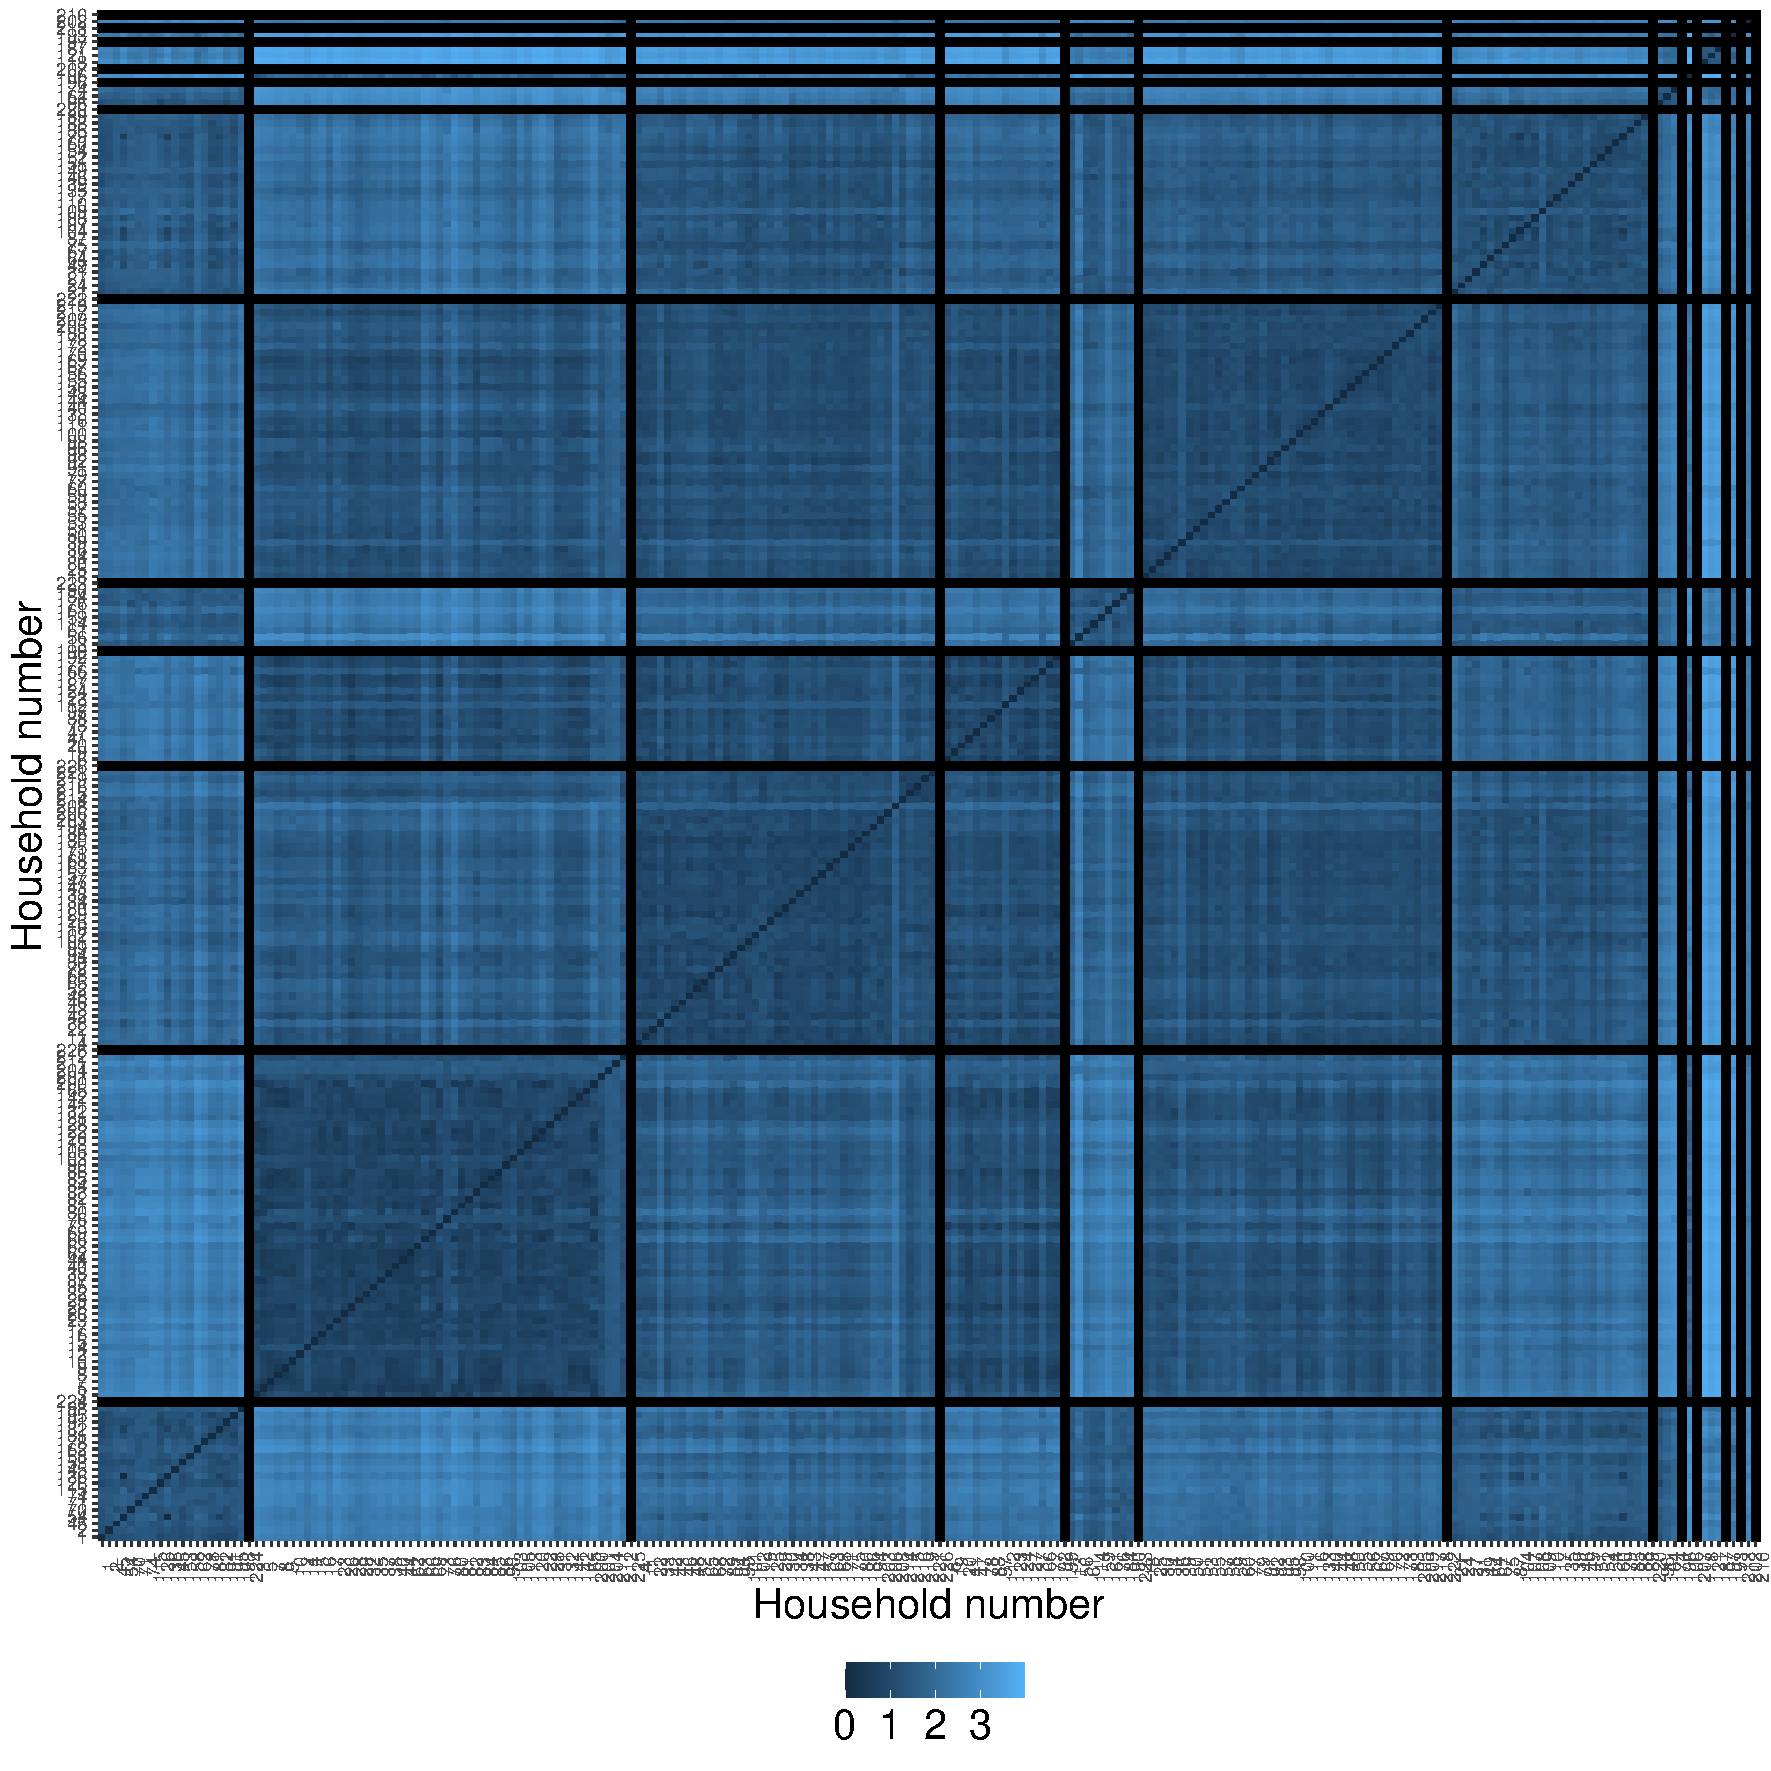
\includegraphics[width = 0.7\textwidth]{heatmap.pdf}
    \caption{Heatmap of DTW distances (transformed to log-scale) between average daily household profiles, arranged according to clusters.}
    \label{fig:heatplot-log}
\end{figure}

One can clearly see that the pairwise within-cluster distances are relatively smaller than the between-cluster distances. Subsequently, for the main analysis, we assume that the electricity demand profiles of two households residing in two different clusters are independent. This allows us to apply the proposed quantile estimator separately on each of the cluster of households and obtain predictions for the quantile profiles for the $9$-th week across all $226$ households. For all households within a cluster, we use the same quantile level for ease of implementation and interpretation, and we use the levels of 0.5, 0.75, 0.8, 0.9, 0.95, 0.99 for every case. After estimating the quantile functions from the training data, the quantile levels for different households in the 12 clusters are predicted and \Cref{fig:estimate-cluster} demonstrates these predicted values.

% \begin{figure}[!ht]
%      \centering
%      \begin{subfigure}[b]{0.48\textwidth}
%          \centering
%          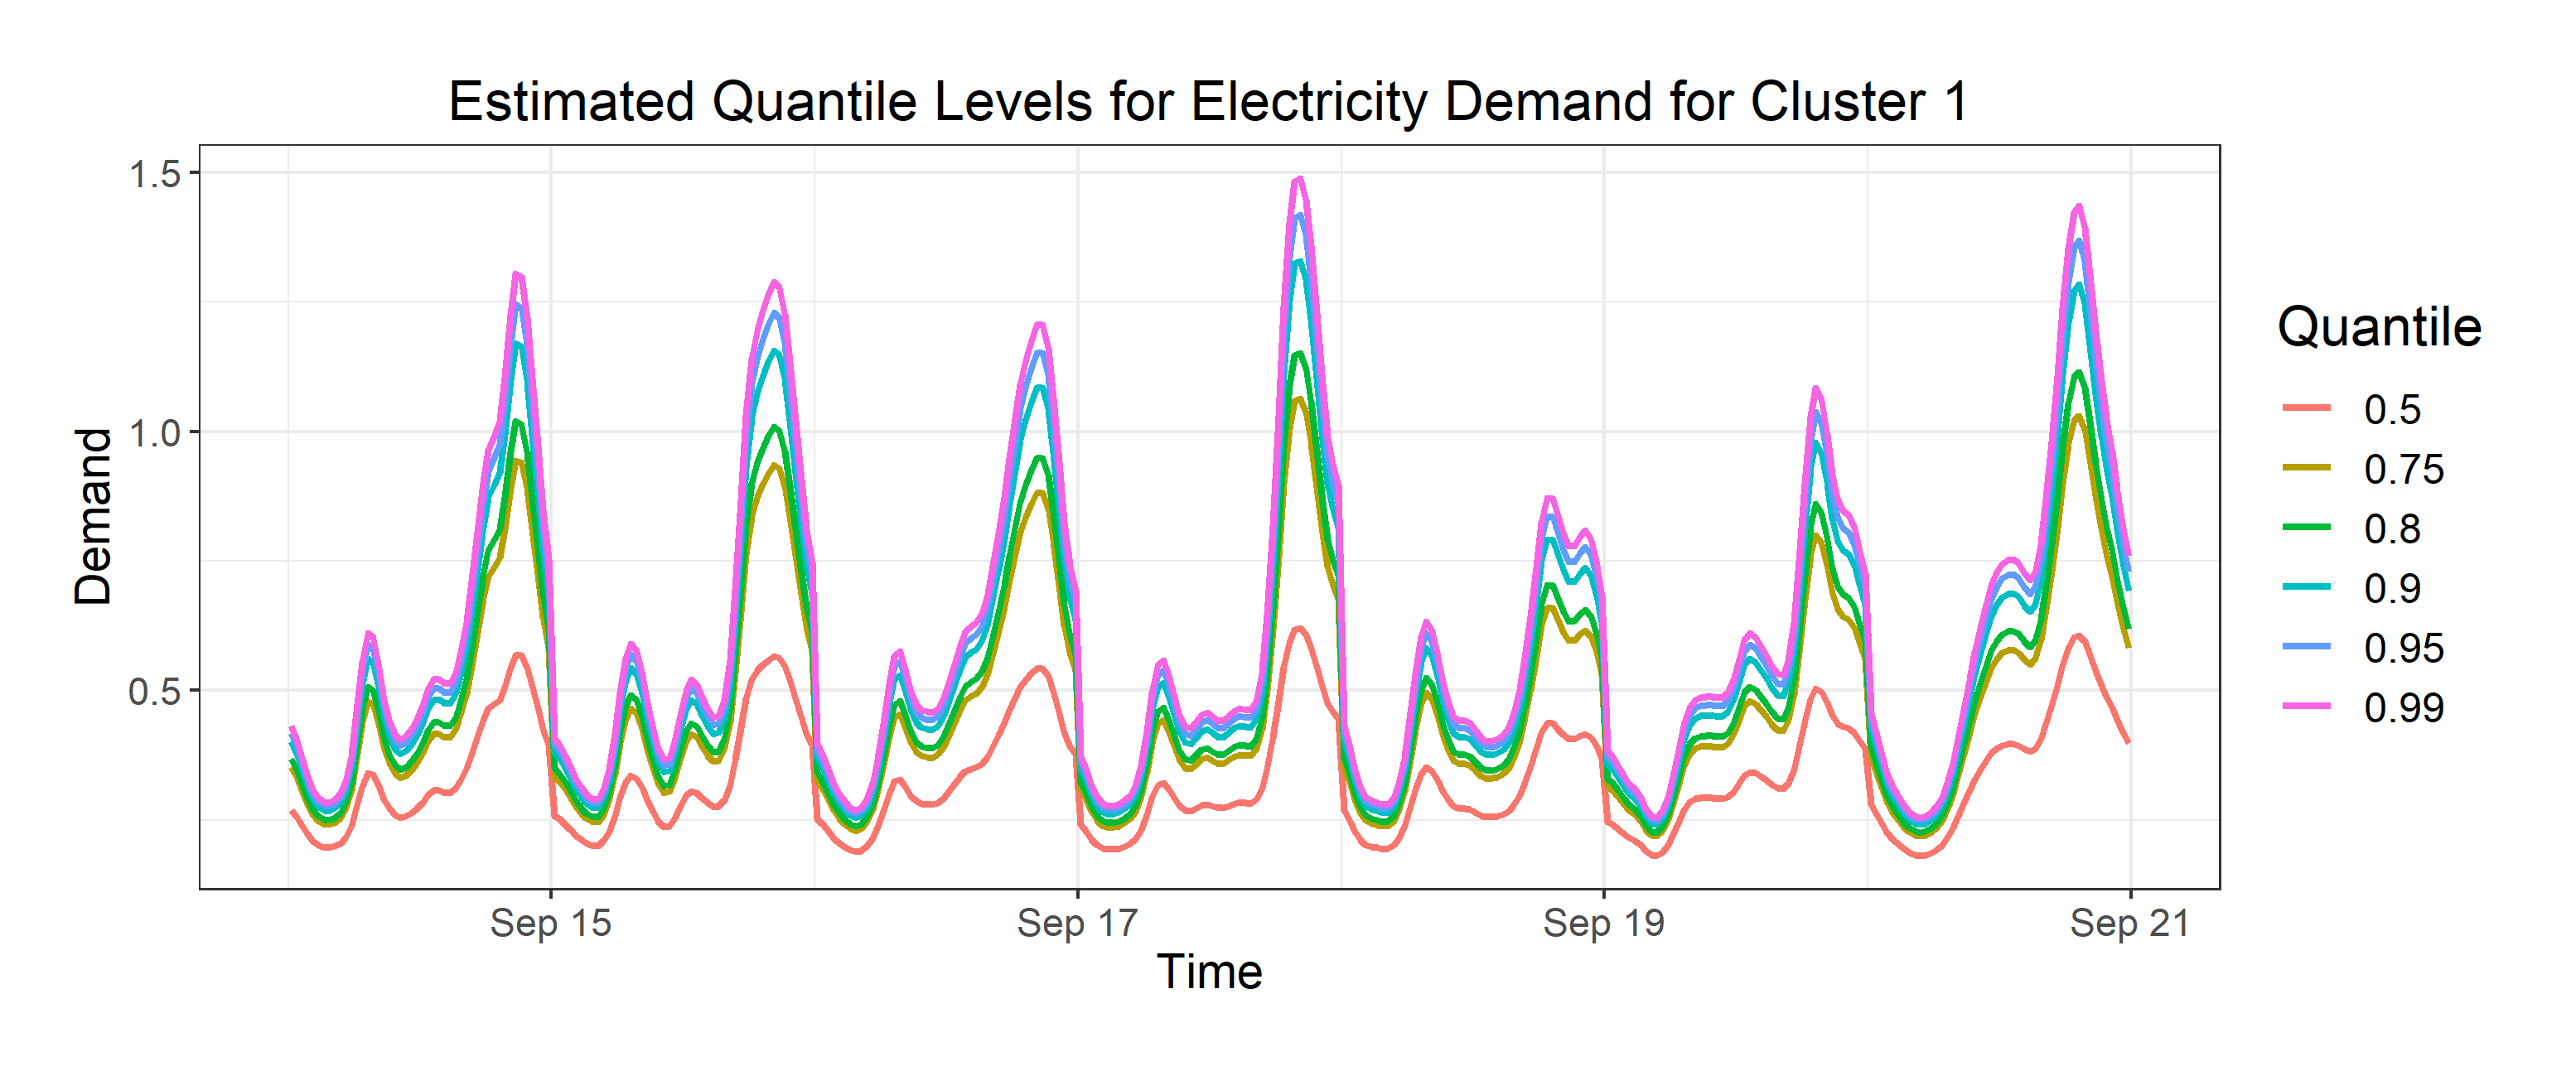
\includegraphics[width=\textwidth]{figures/quantlevel-1.png}
%      \end{subfigure}
%      \hfill
%      \begin{subfigure}[b]{0.48\textwidth}
%          \centering
%          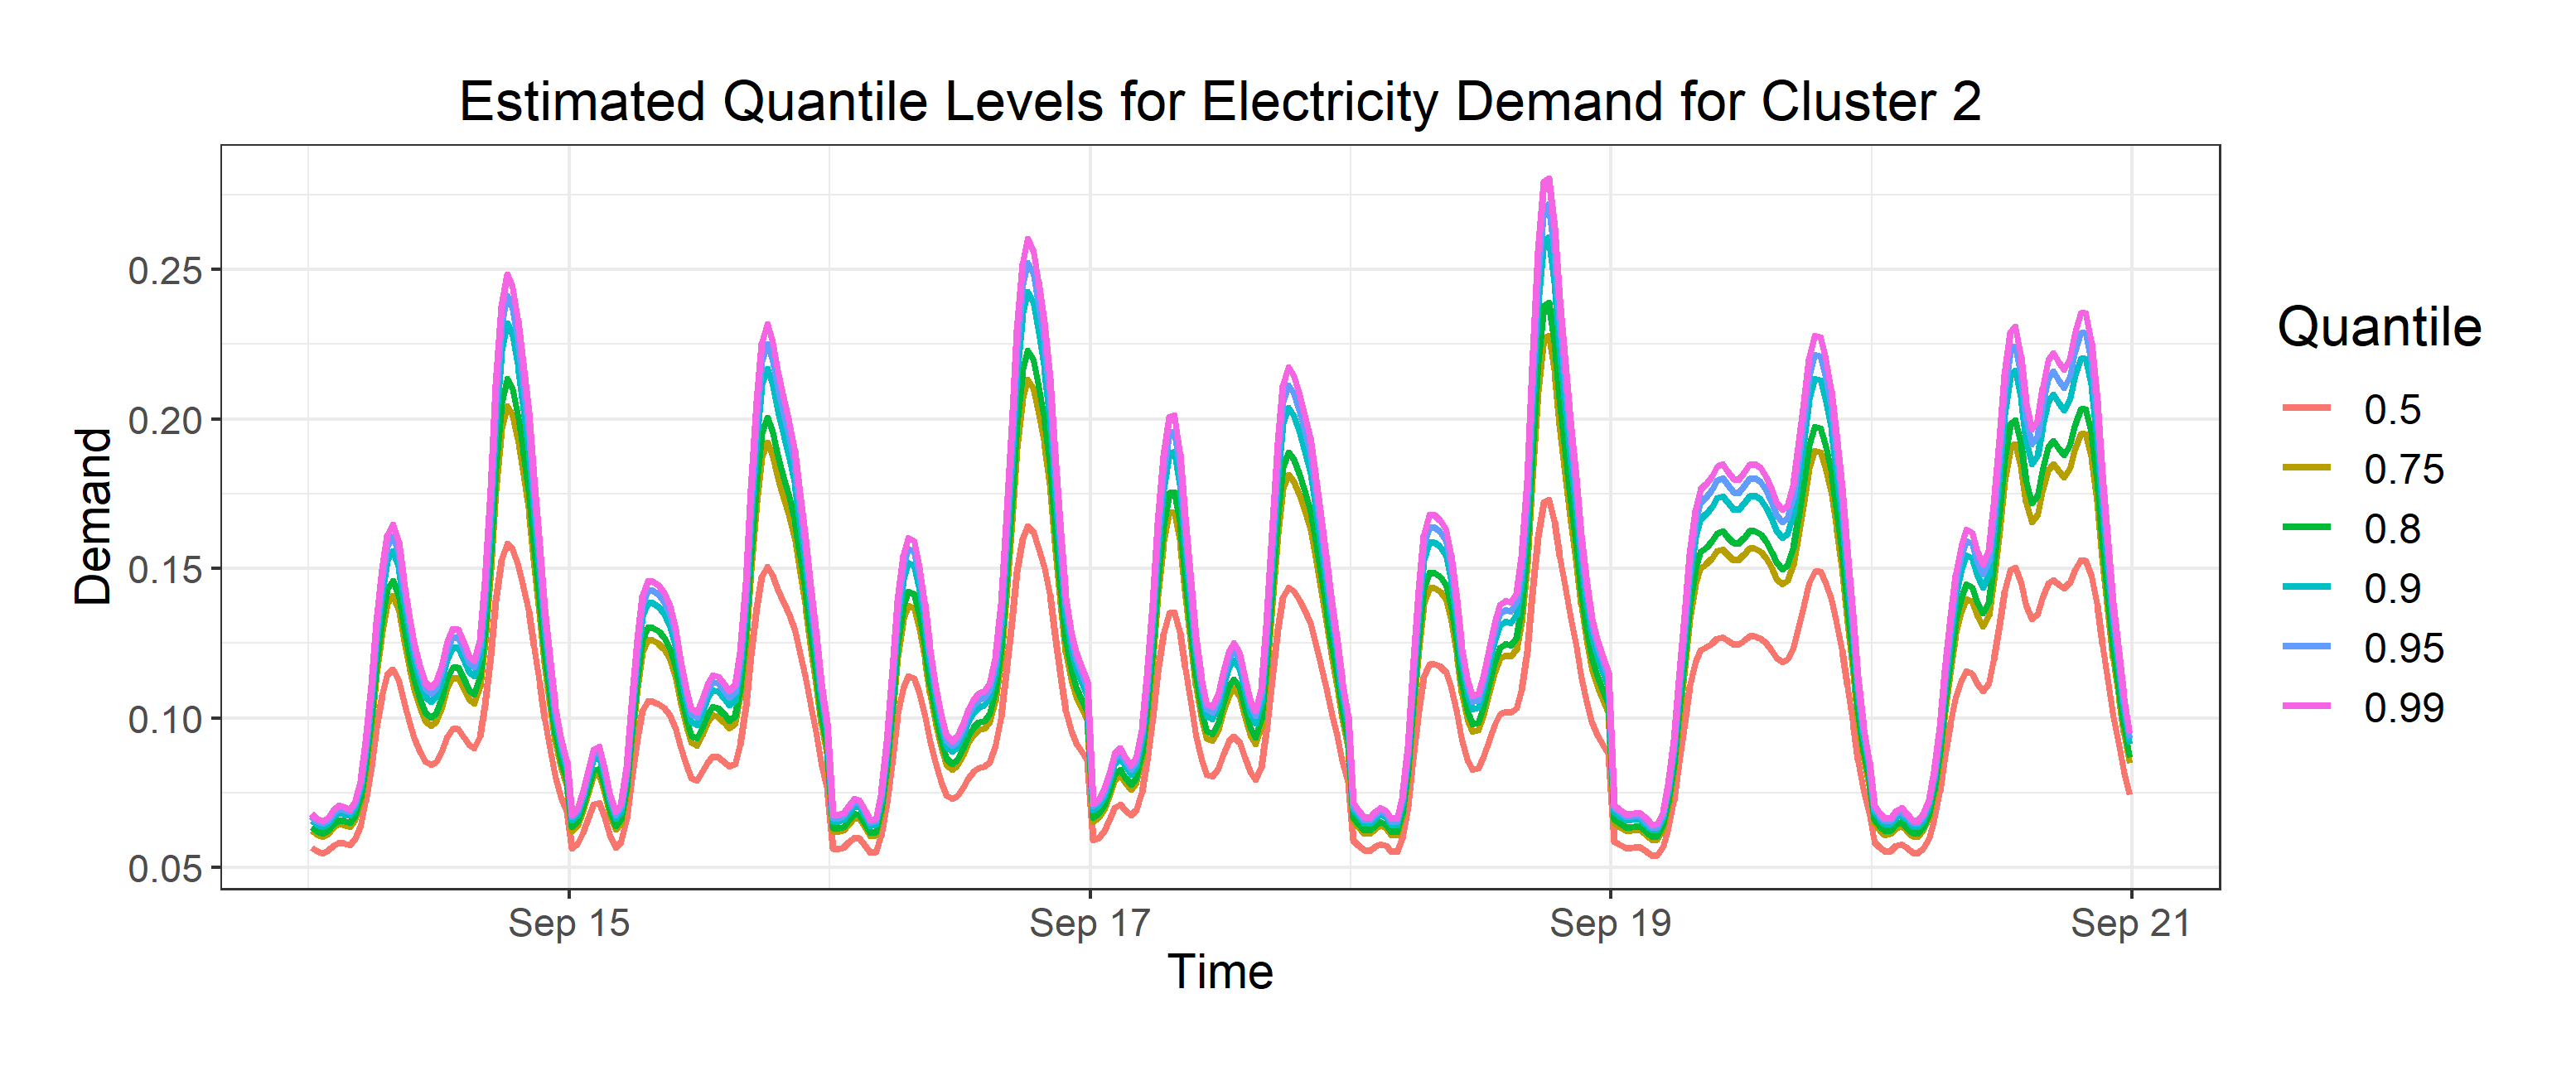
\includegraphics[width=\textwidth]{figures/quantlevel-2.png}
%      \end{subfigure}
%      \hfill
%      \begin{subfigure}[b]{0.48\textwidth}
%          \centering
%          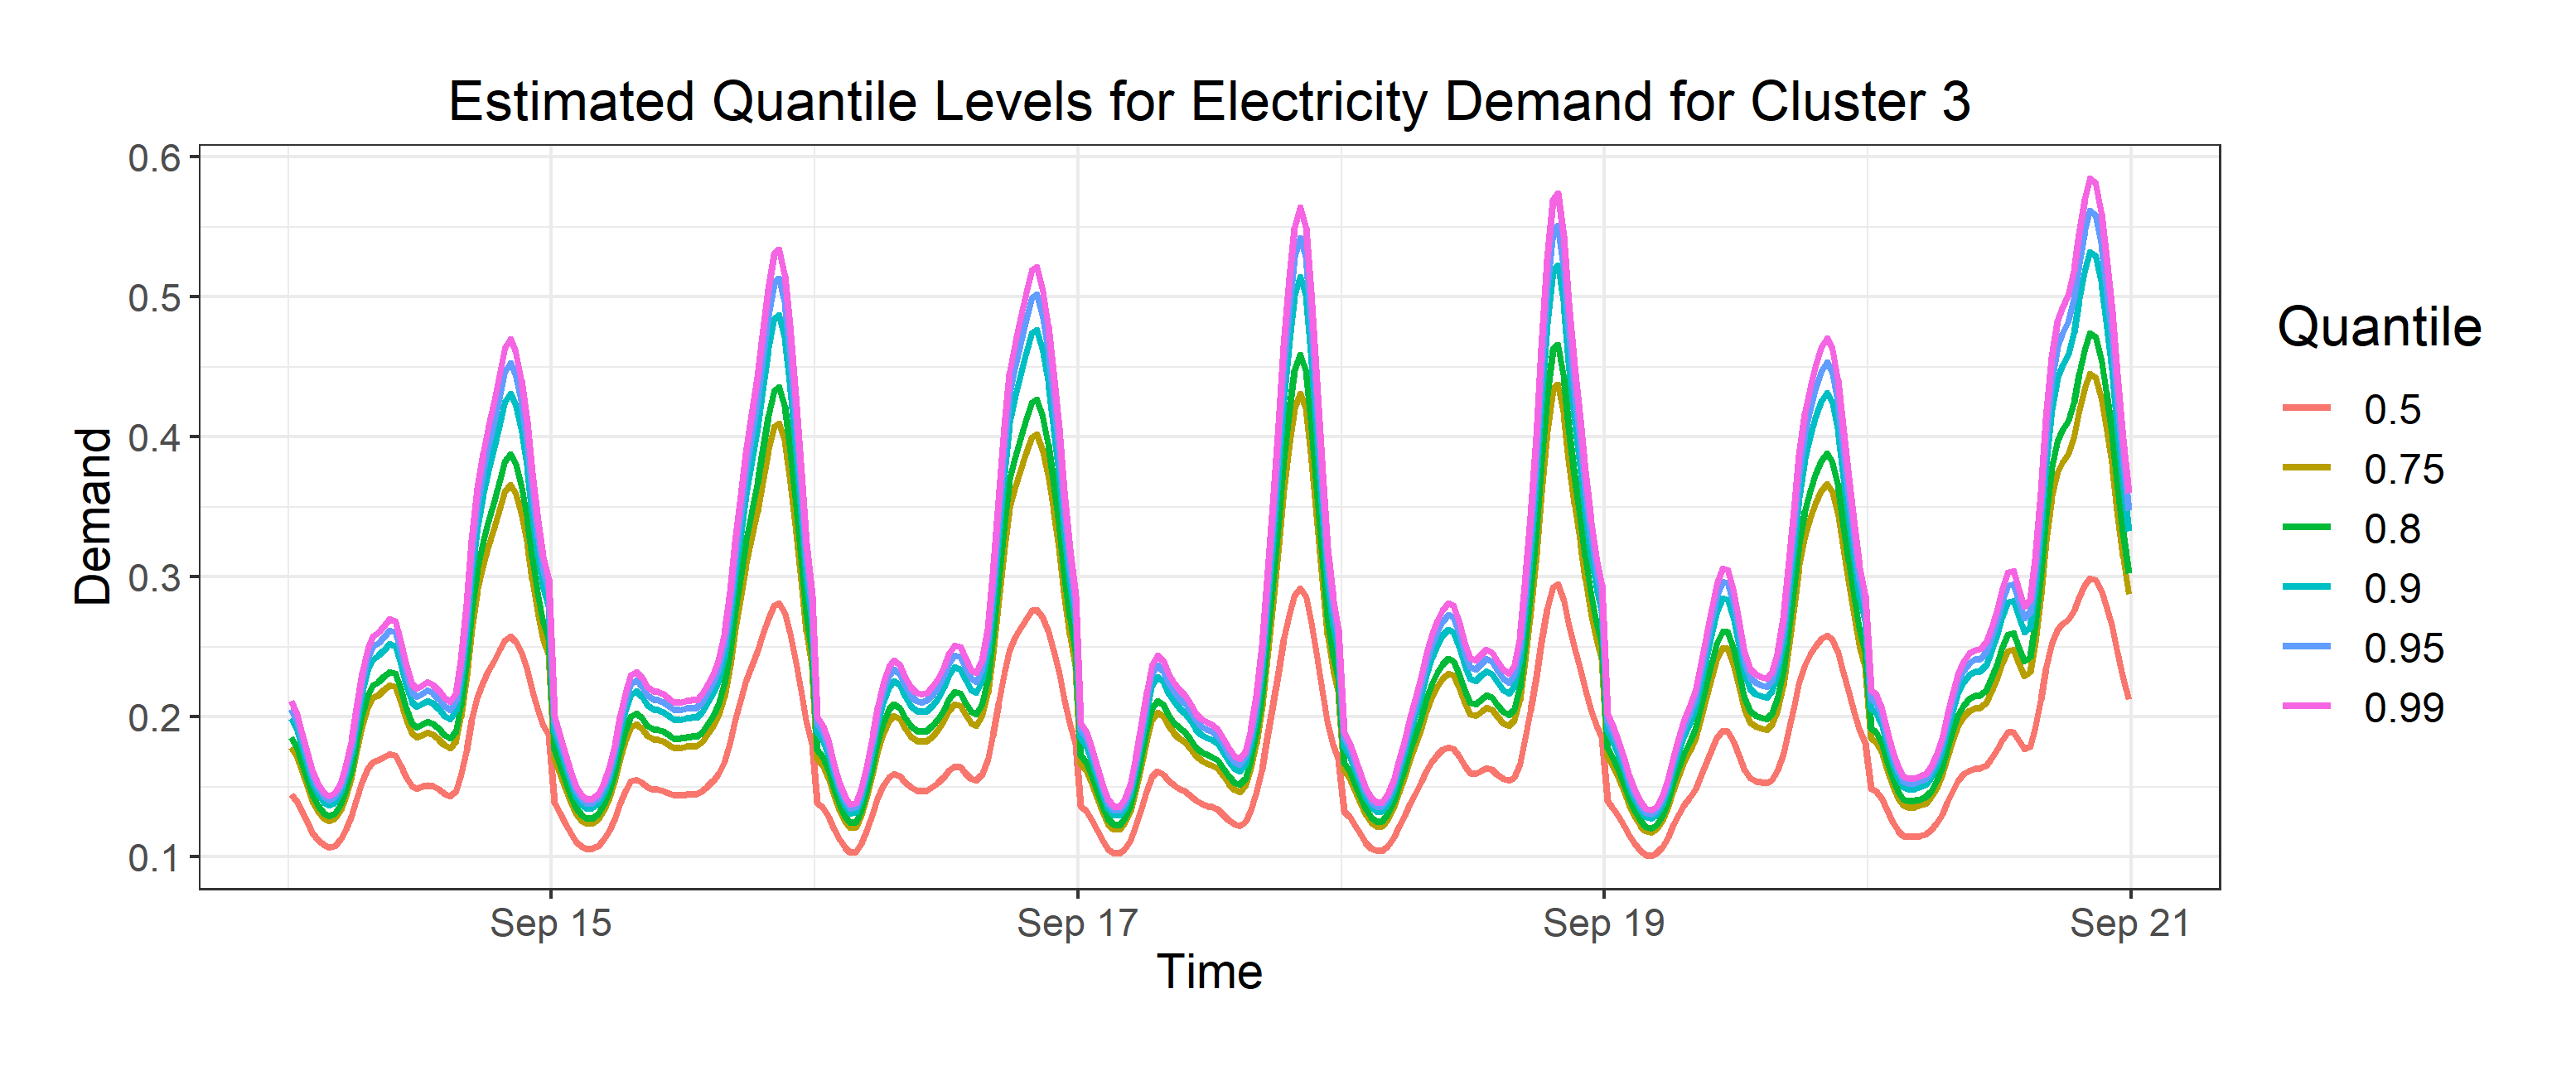
\includegraphics[width=\textwidth]{figures/quantlevel-3.png}
%      \end{subfigure}
%      \begin{subfigure}[b]{0.48\textwidth}
%          \centering
%          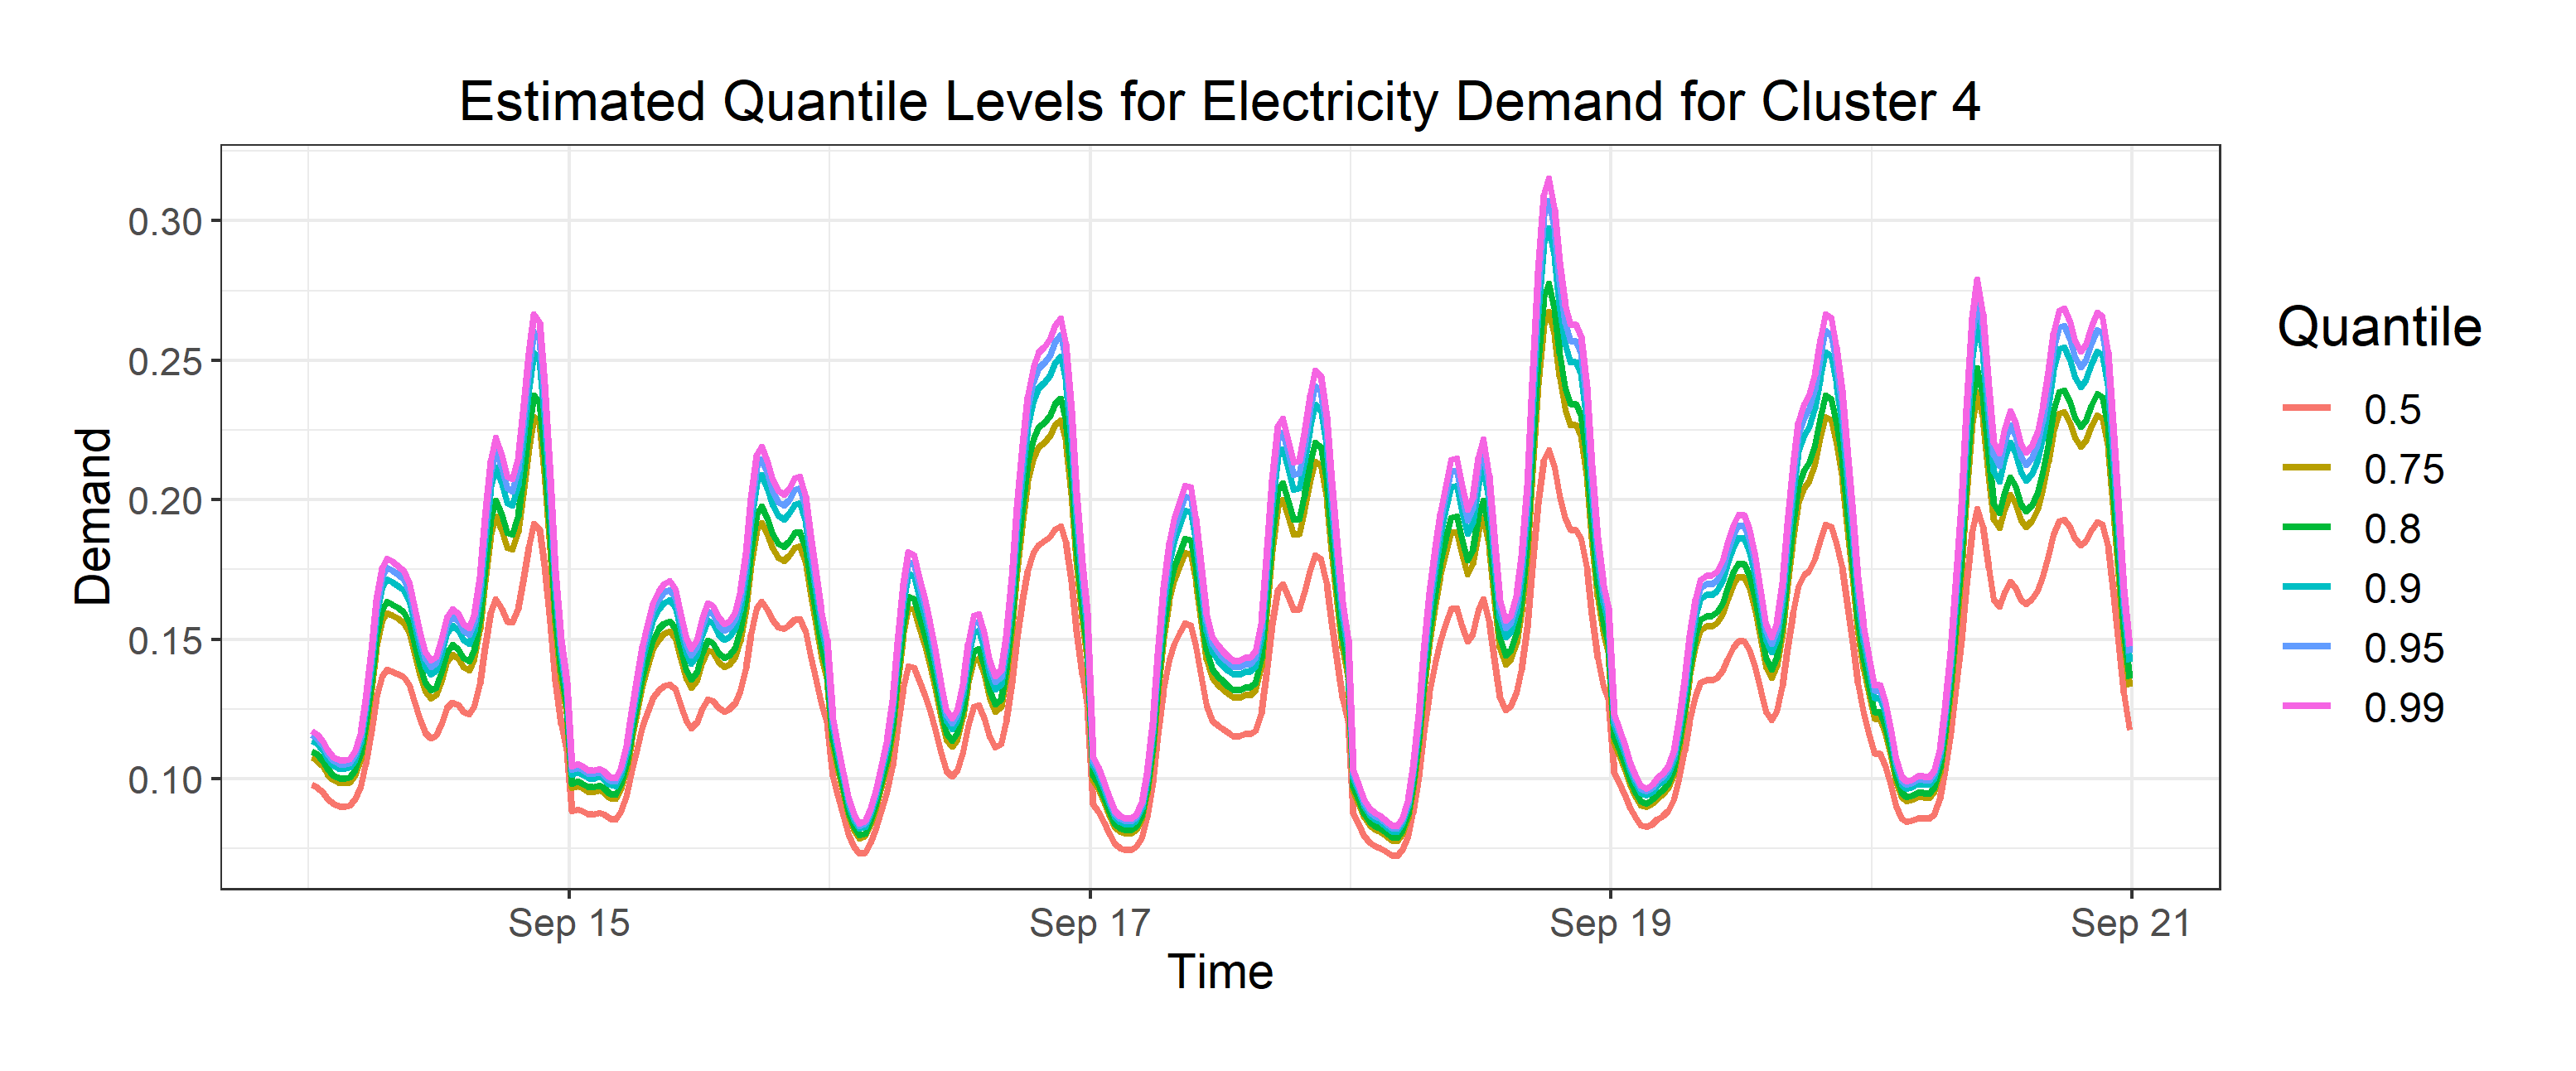
\includegraphics[width=\textwidth]{figures/quantlevel-4.png}
%      \end{subfigure}
%      \hfill
%      \begin{subfigure}[b]{0.48\textwidth}
%          \centering
%          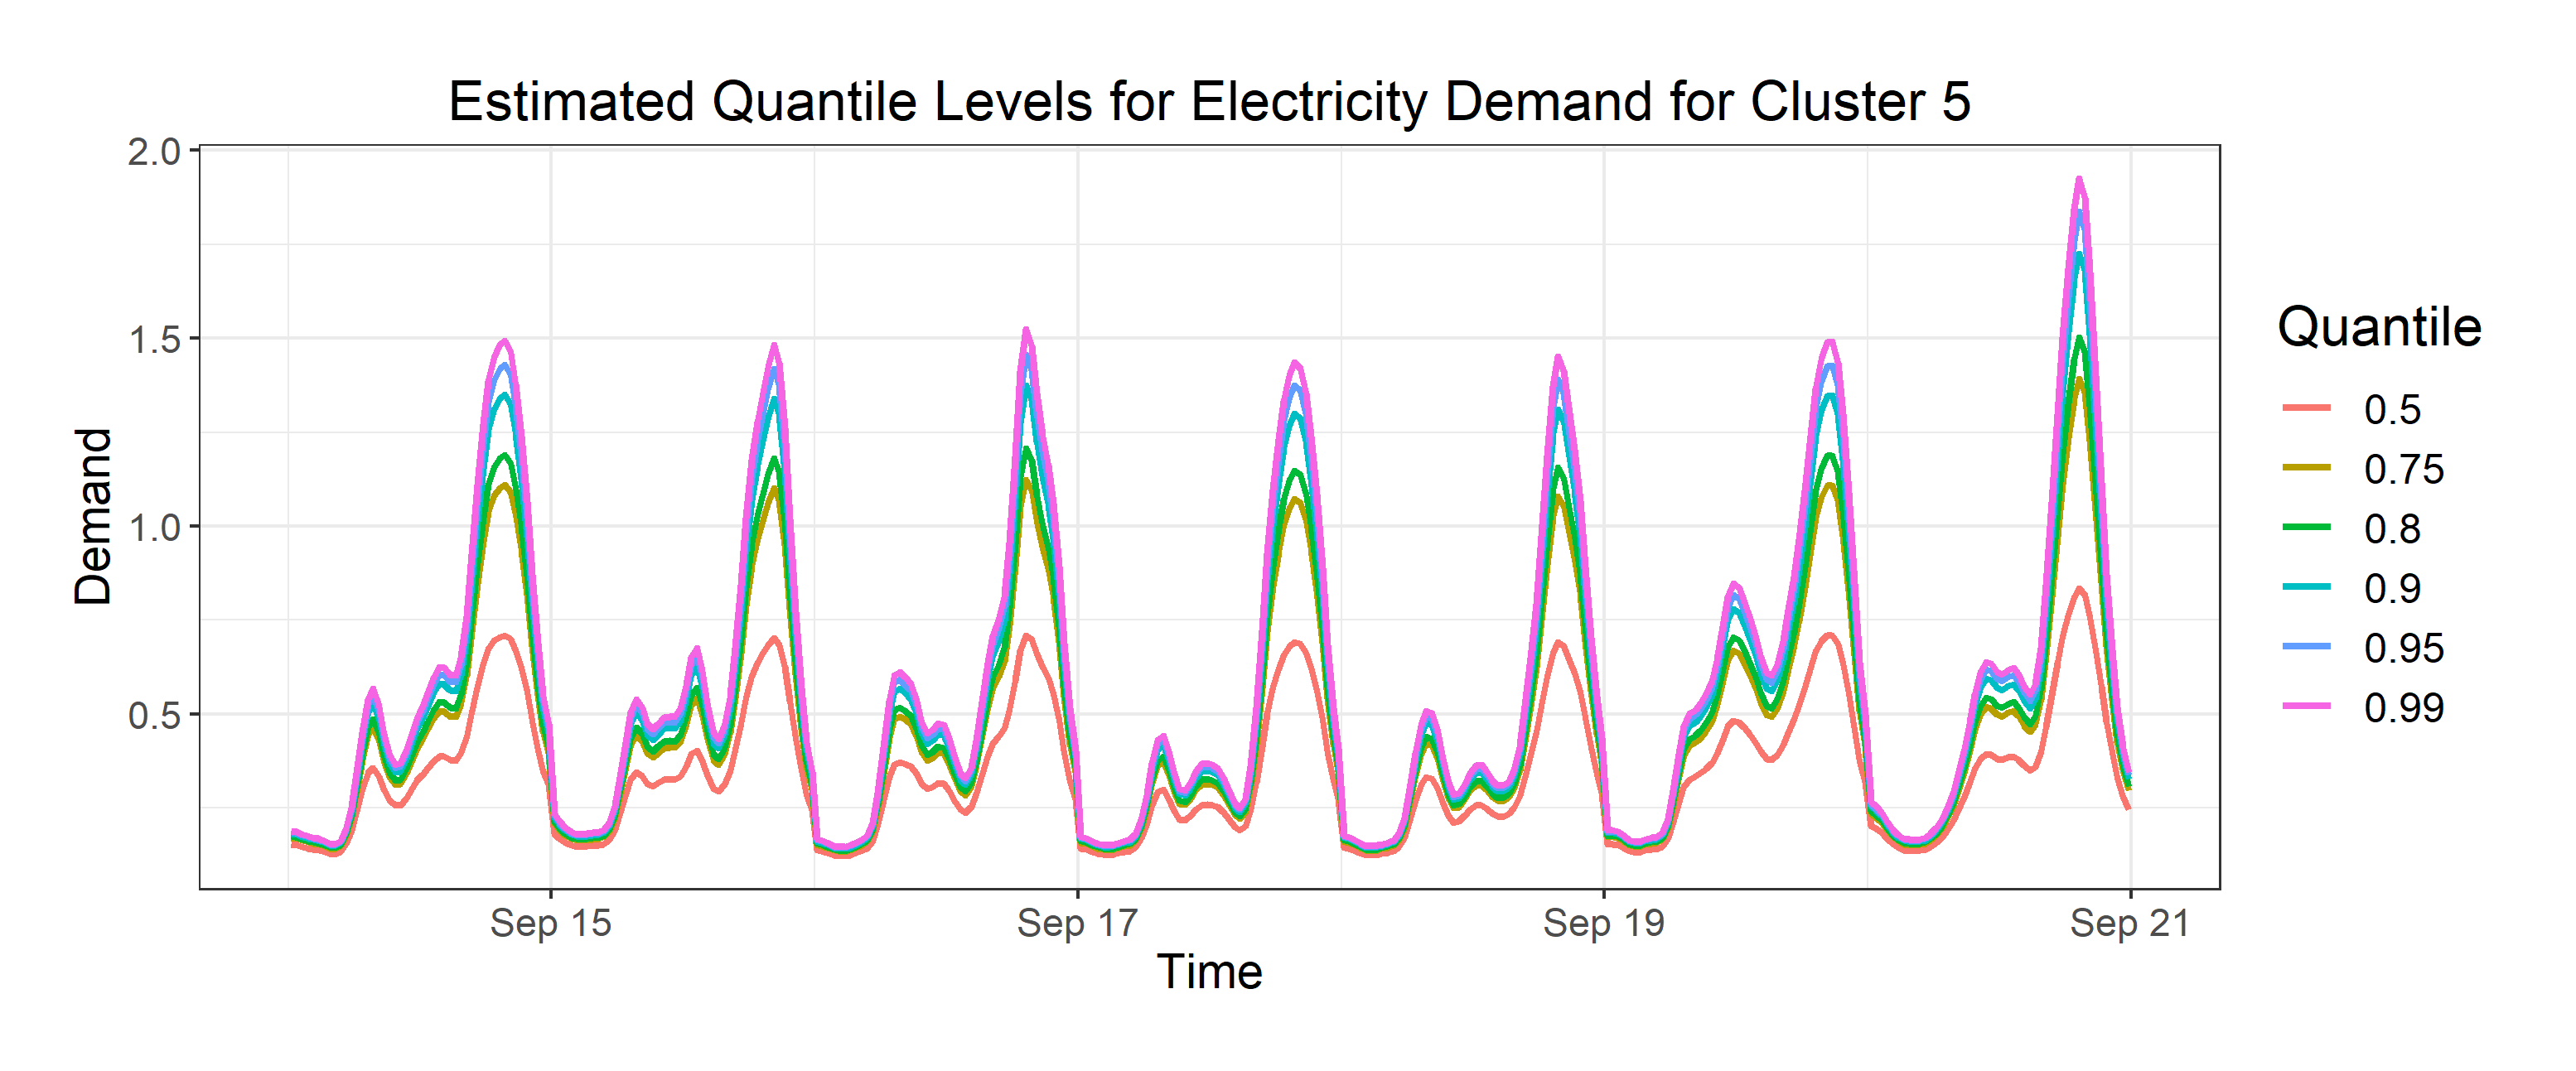
\includegraphics[width=\textwidth]{figures/quantlevel-5.png}
%      \end{subfigure}
%      \hfill
%      \begin{subfigure}[b]{0.48\textwidth}
%          \centering
%          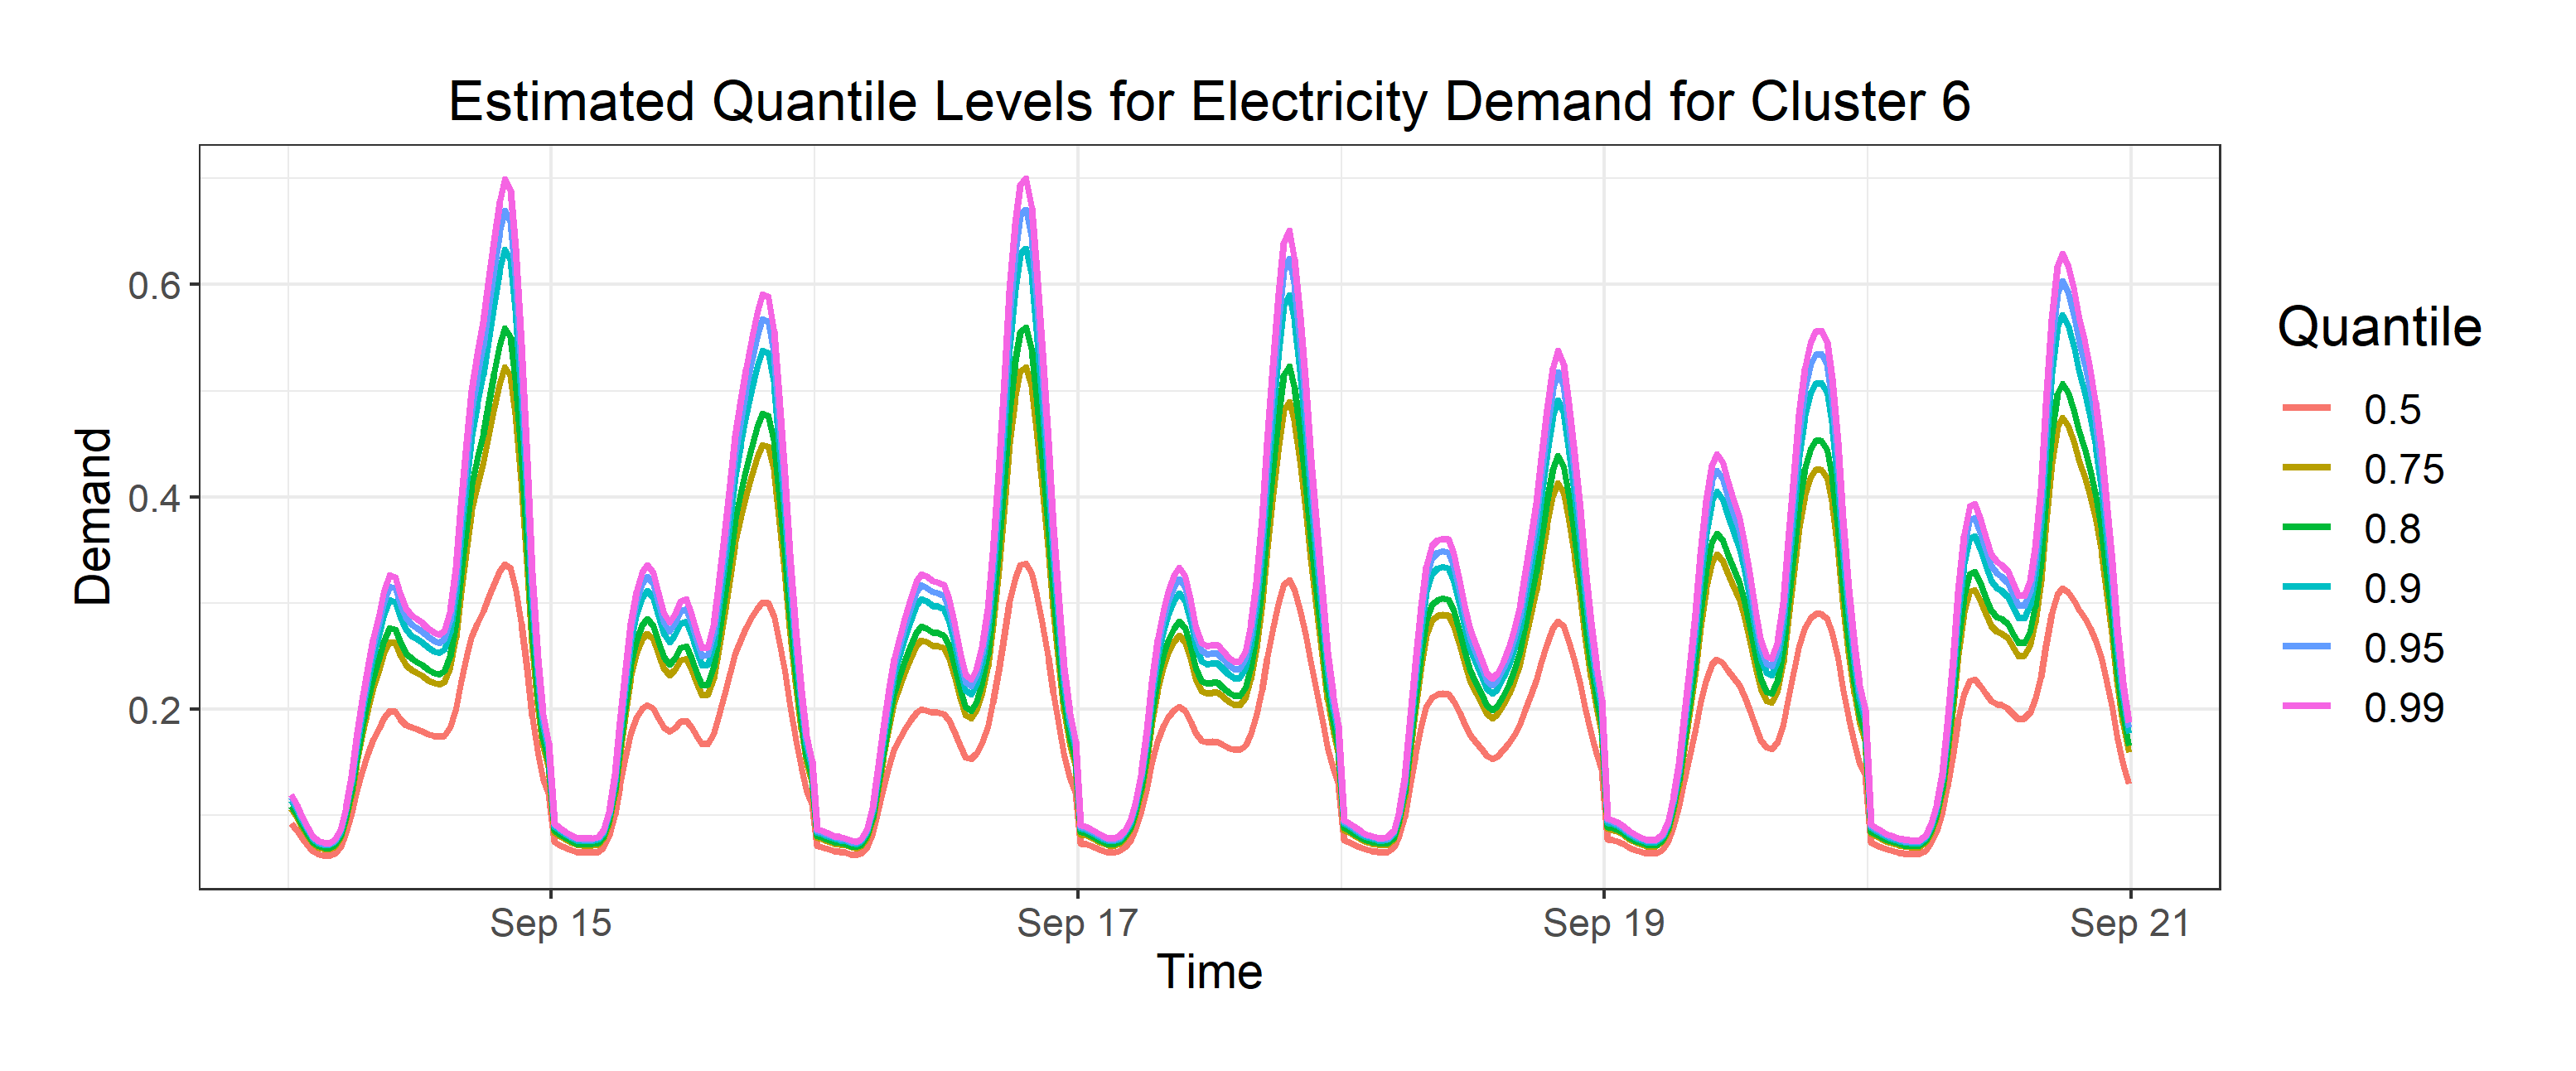
\includegraphics[width=\textwidth]{figures/quantlevel-6.png}
%      \end{subfigure}
%      \begin{subfigure}[b]{0.48\textwidth}
%          \centering
%          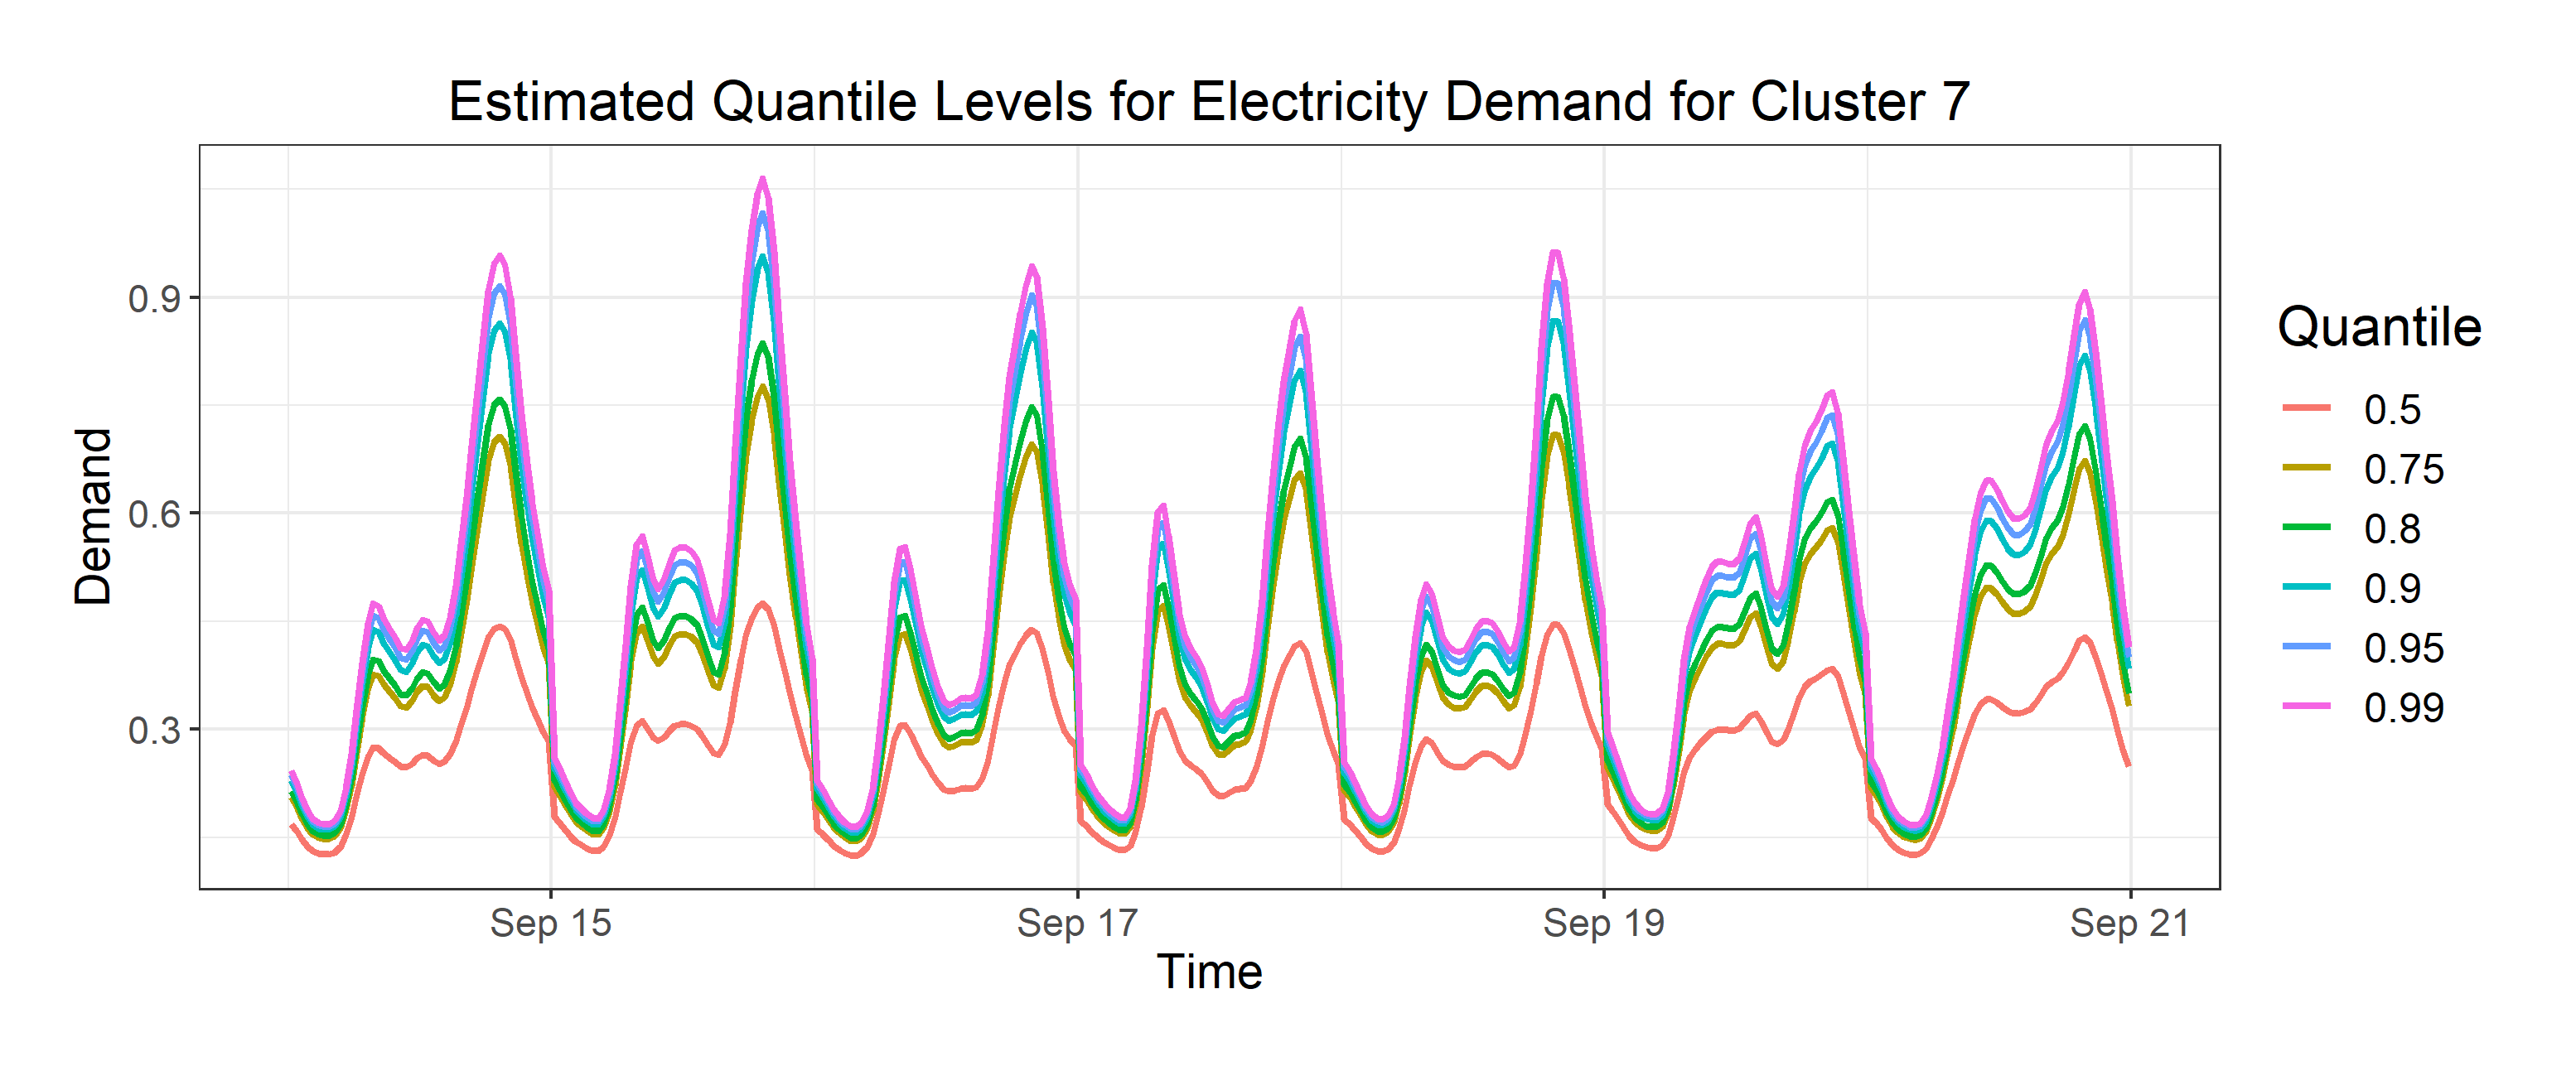
\includegraphics[width=\textwidth]{figures/quantlevel-7.png}
%      \end{subfigure}
%      \hfill
%      \begin{subfigure}[b]{0.48\textwidth}
%          \centering
%          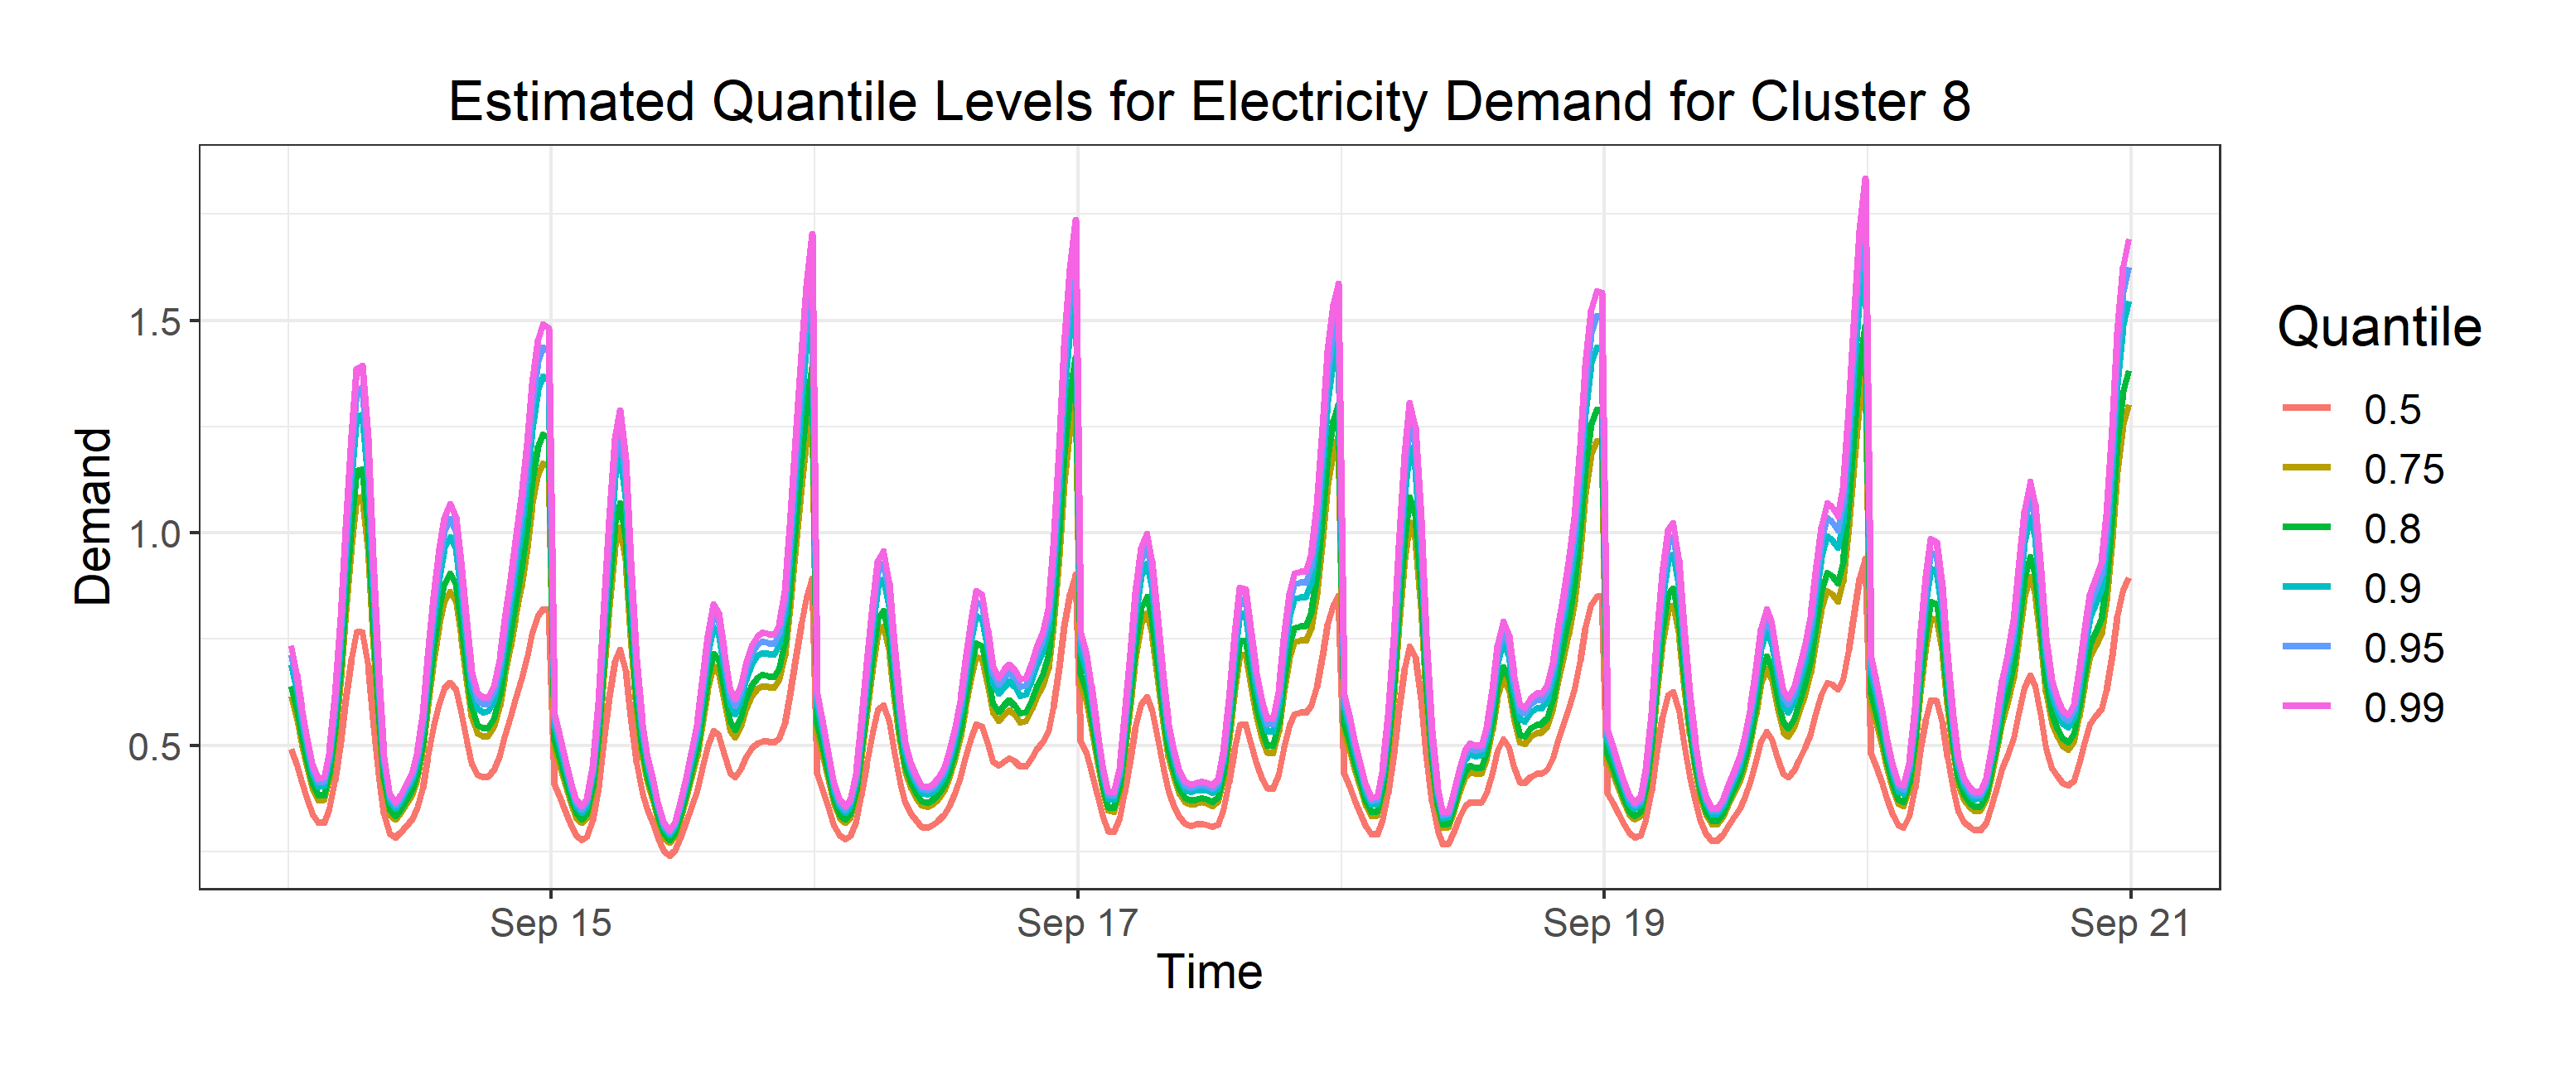
\includegraphics[width=\textwidth]{figures/quantlevel-8.png}
%      \end{subfigure}
%      \hfill
%      \begin{subfigure}[b]{0.48\textwidth}
%          \centering
%          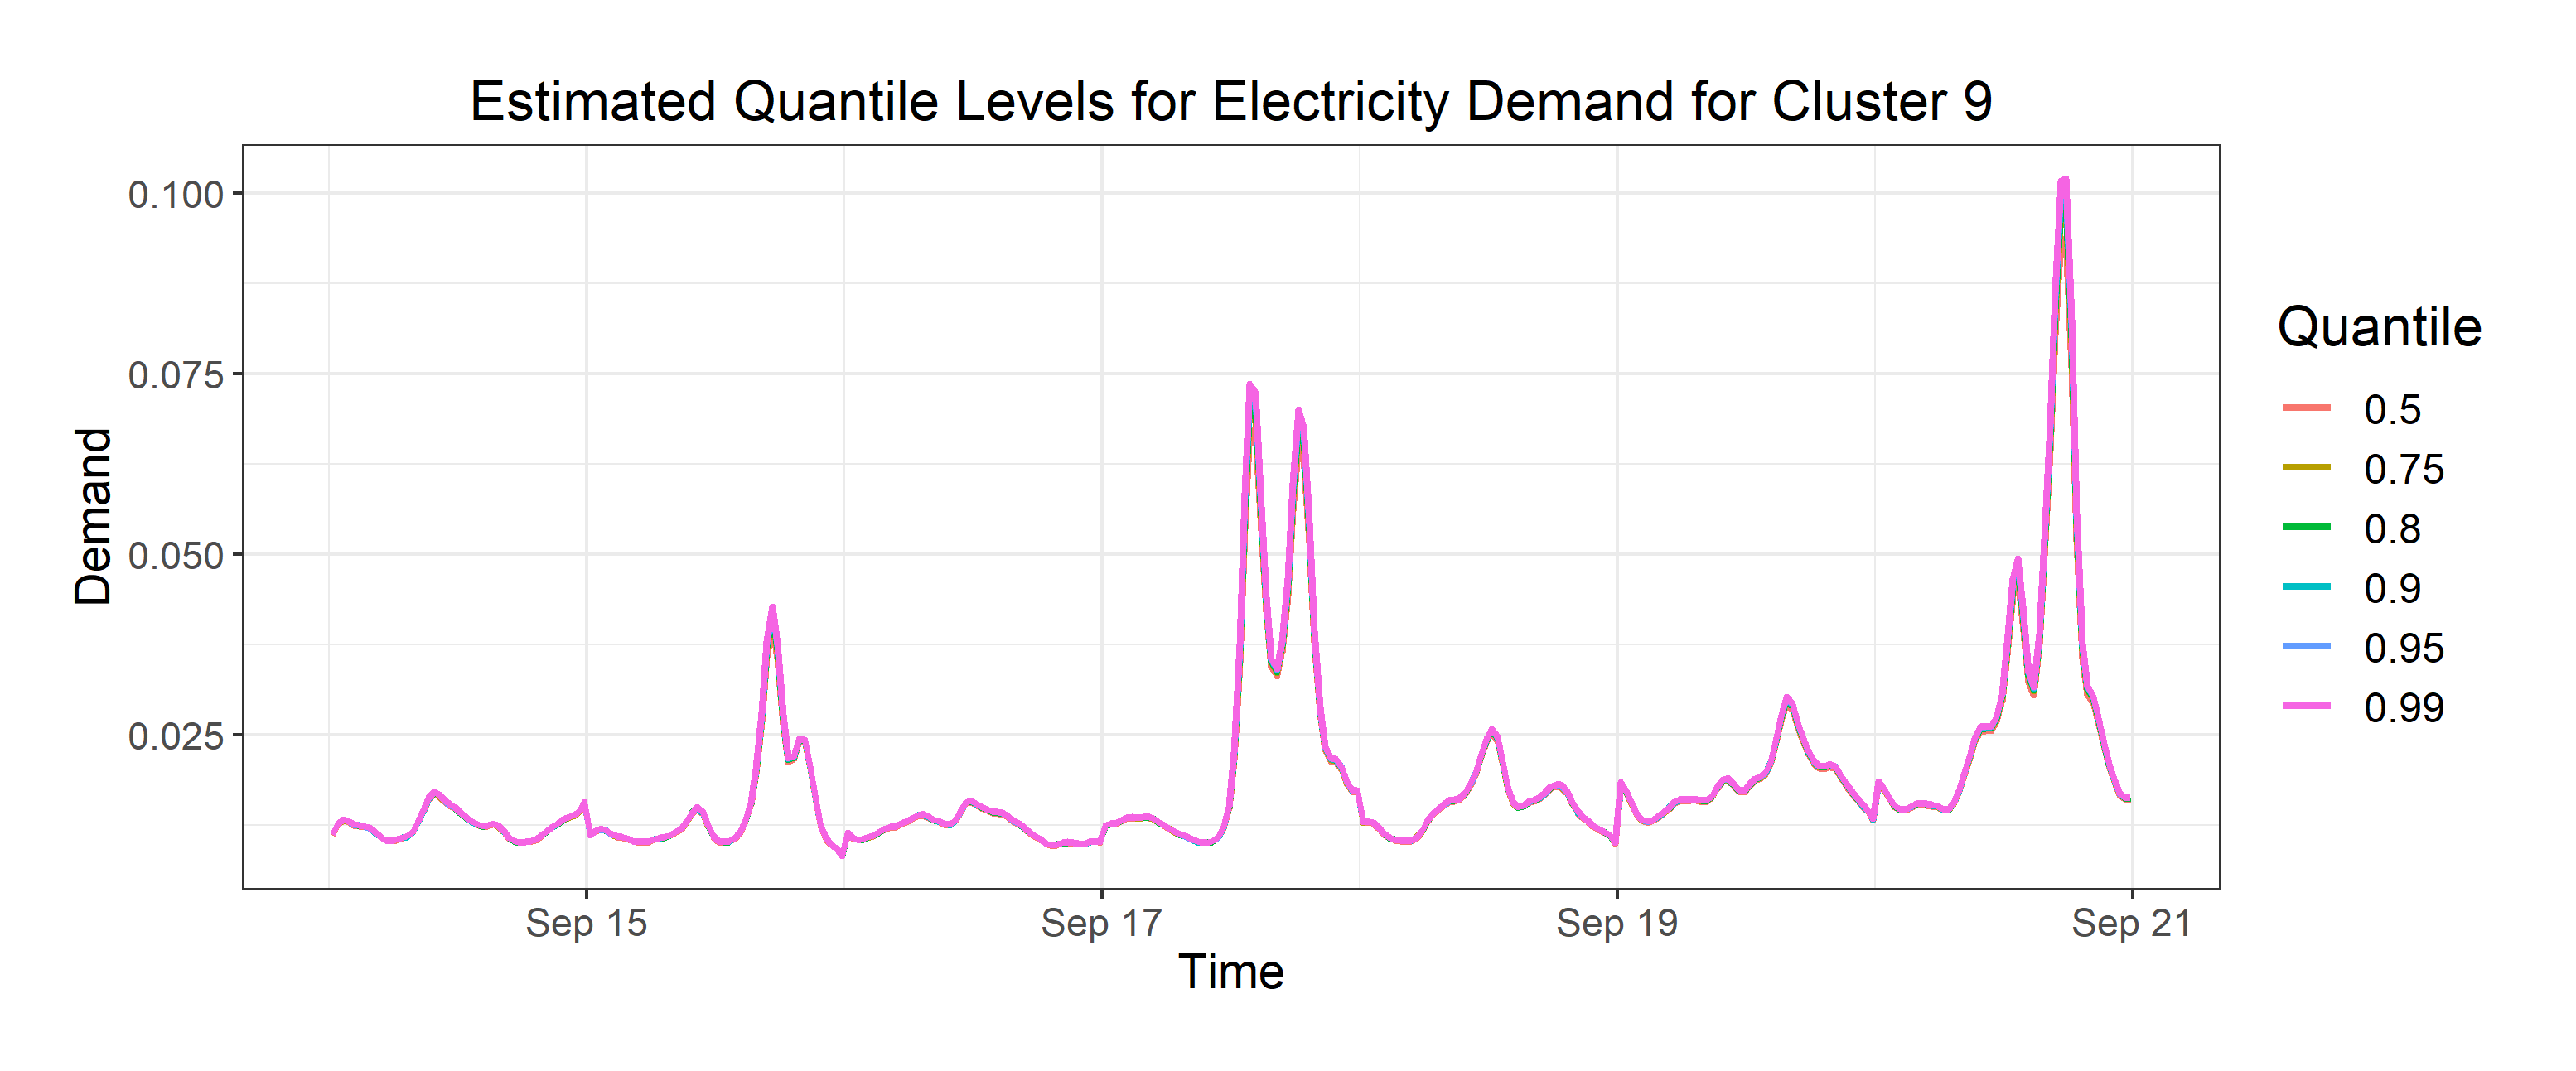
\includegraphics[width=\textwidth]{figures/quantlevel-9.png}
%      \end{subfigure}
%      \begin{subfigure}[b]{0.48\textwidth}
%          \centering
%          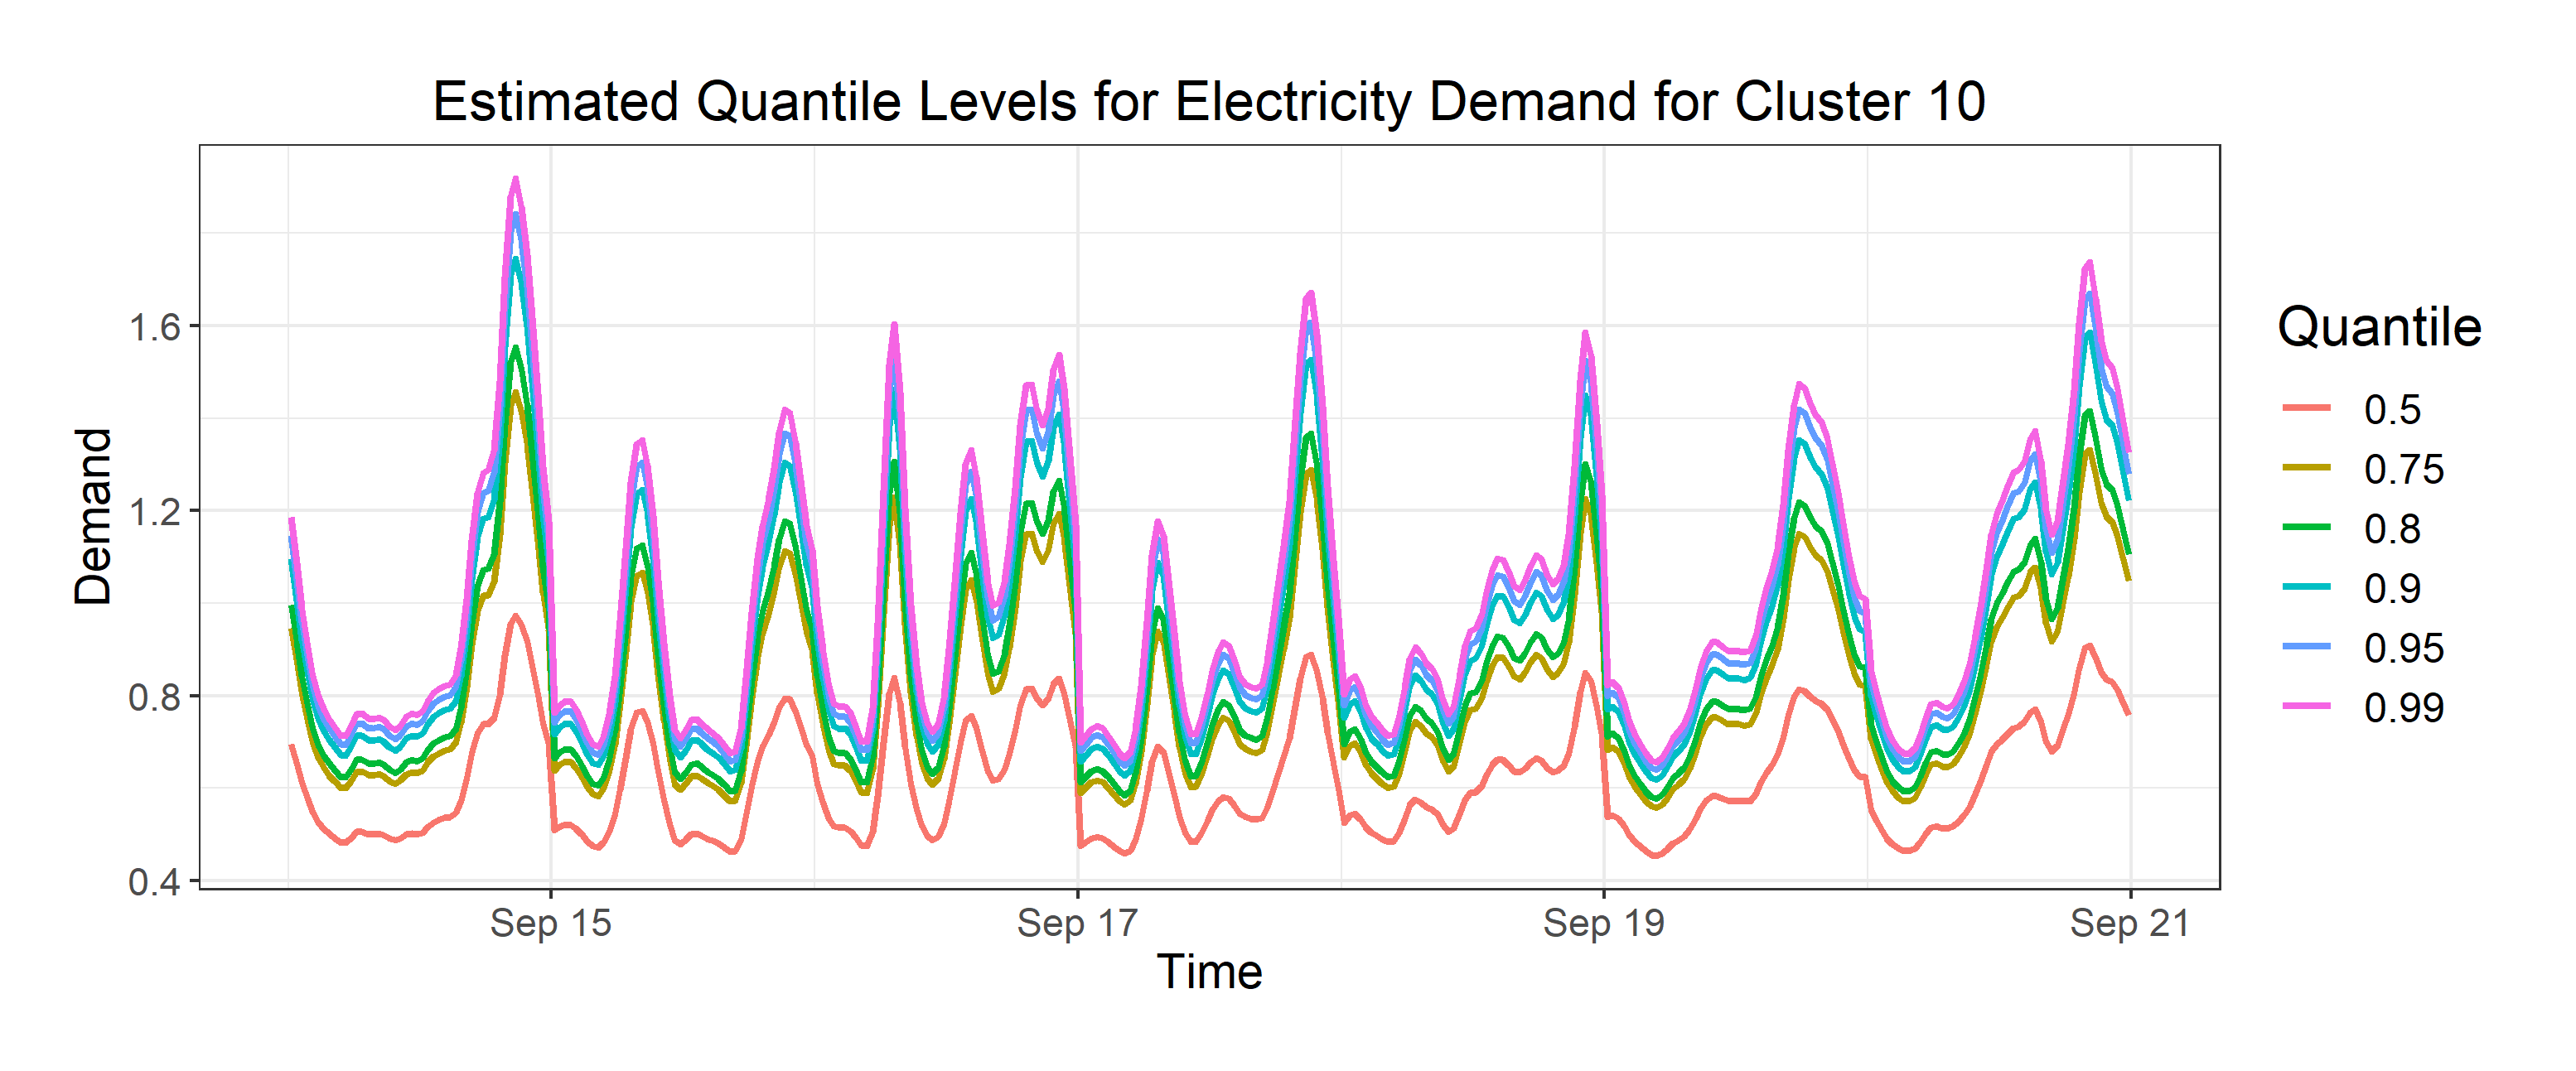
\includegraphics[width=\textwidth]{figures/quantlevel-10.png}
%      \end{subfigure}
%      \hfill
%      \begin{subfigure}[b]{0.48\textwidth}
%          \centering
%          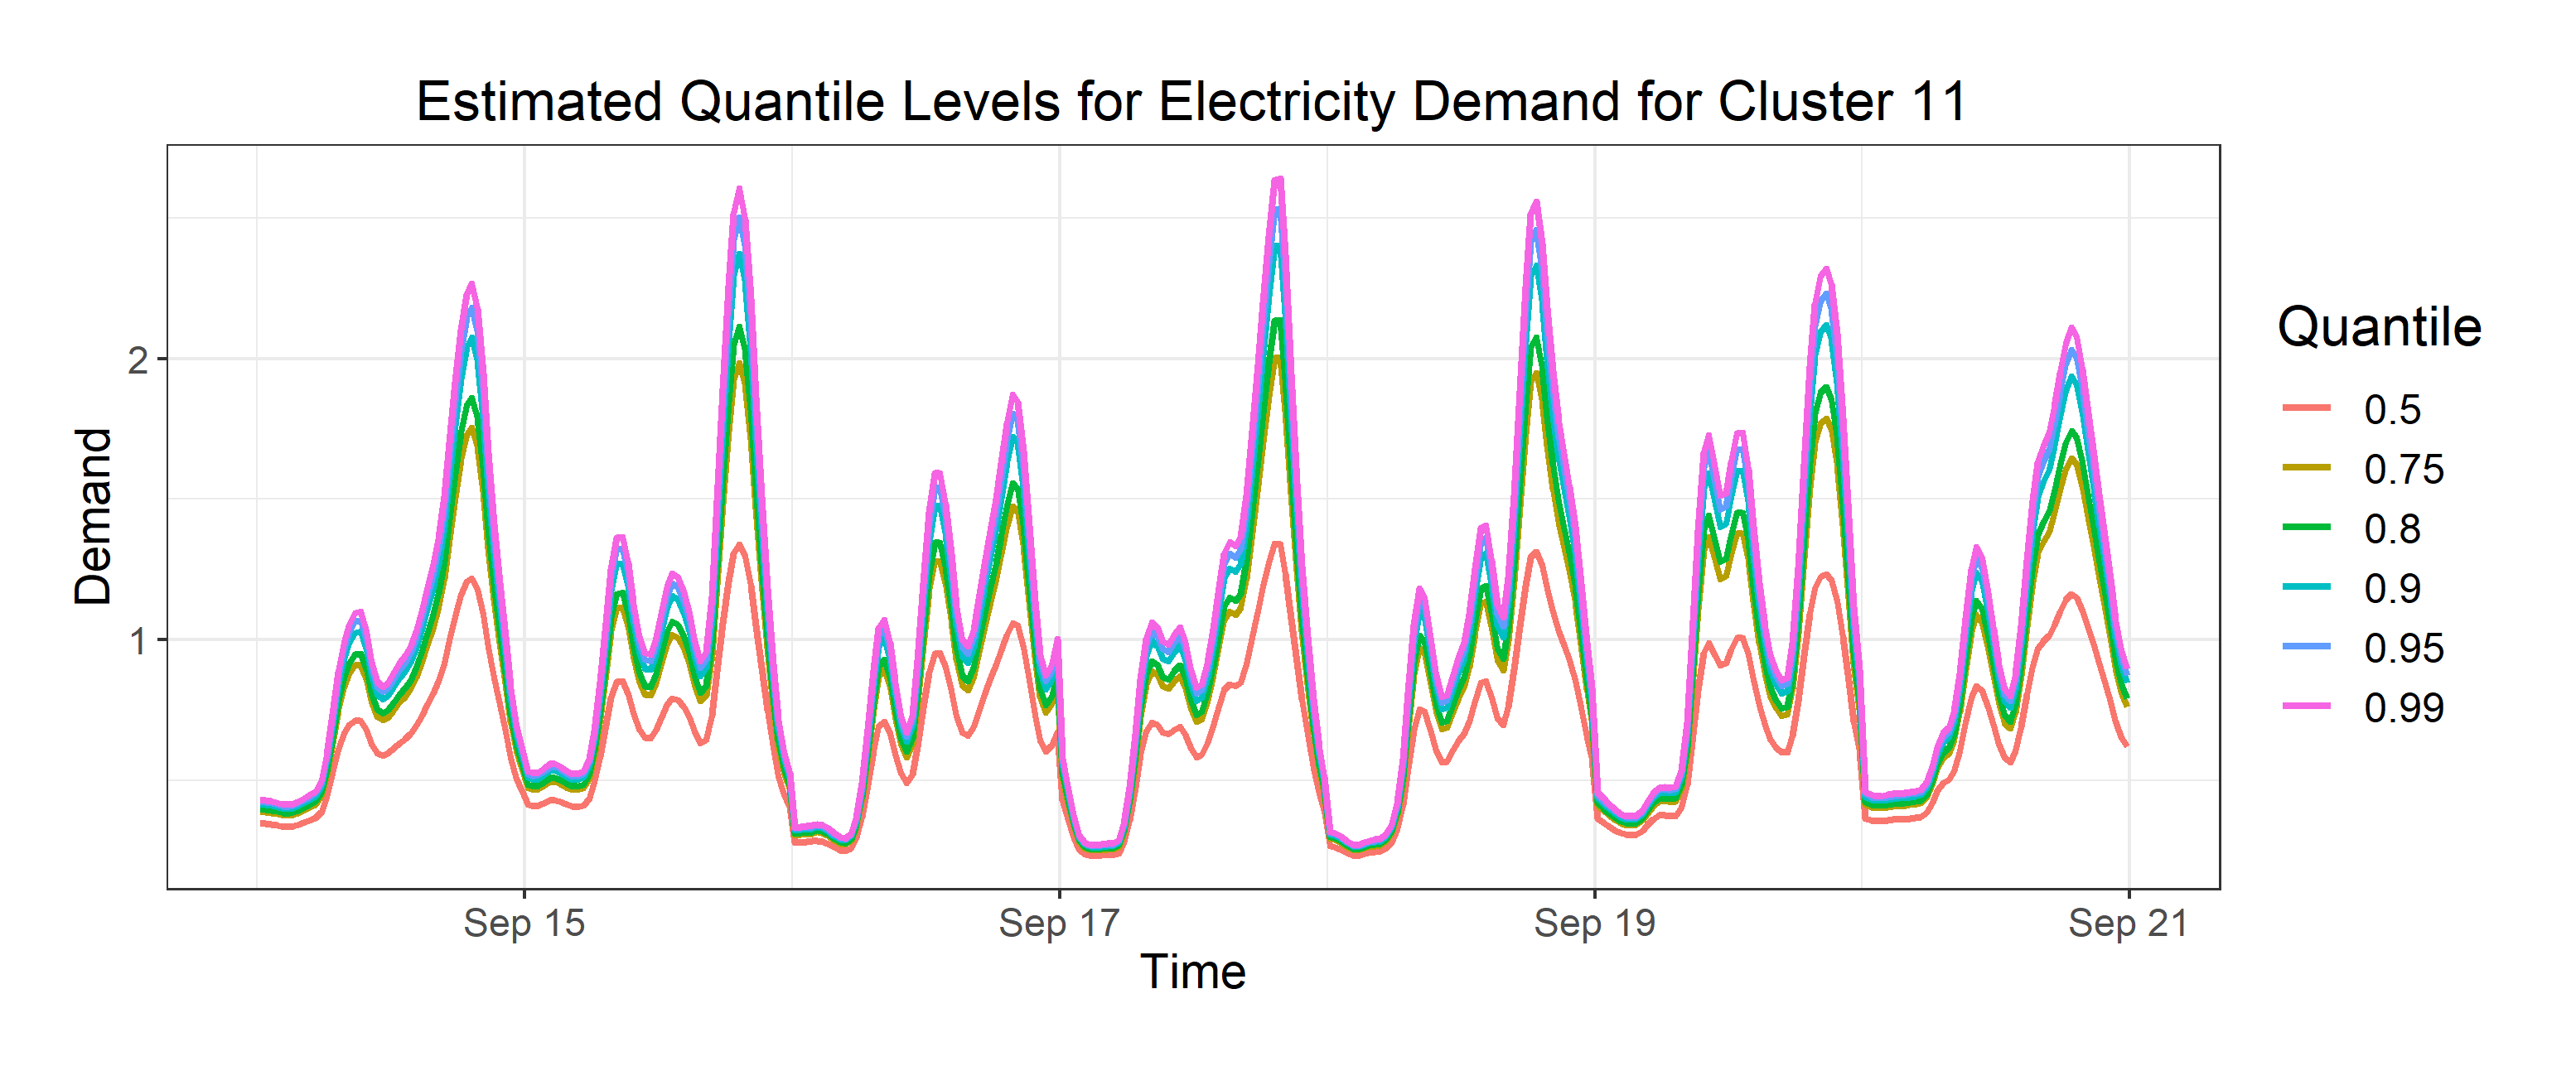
\includegraphics[width=\textwidth]{figures/quantlevel-11.png}
%      \end{subfigure}
%      \hfill
%      \begin{subfigure}[b]{0.48\textwidth}
%          \centering
%          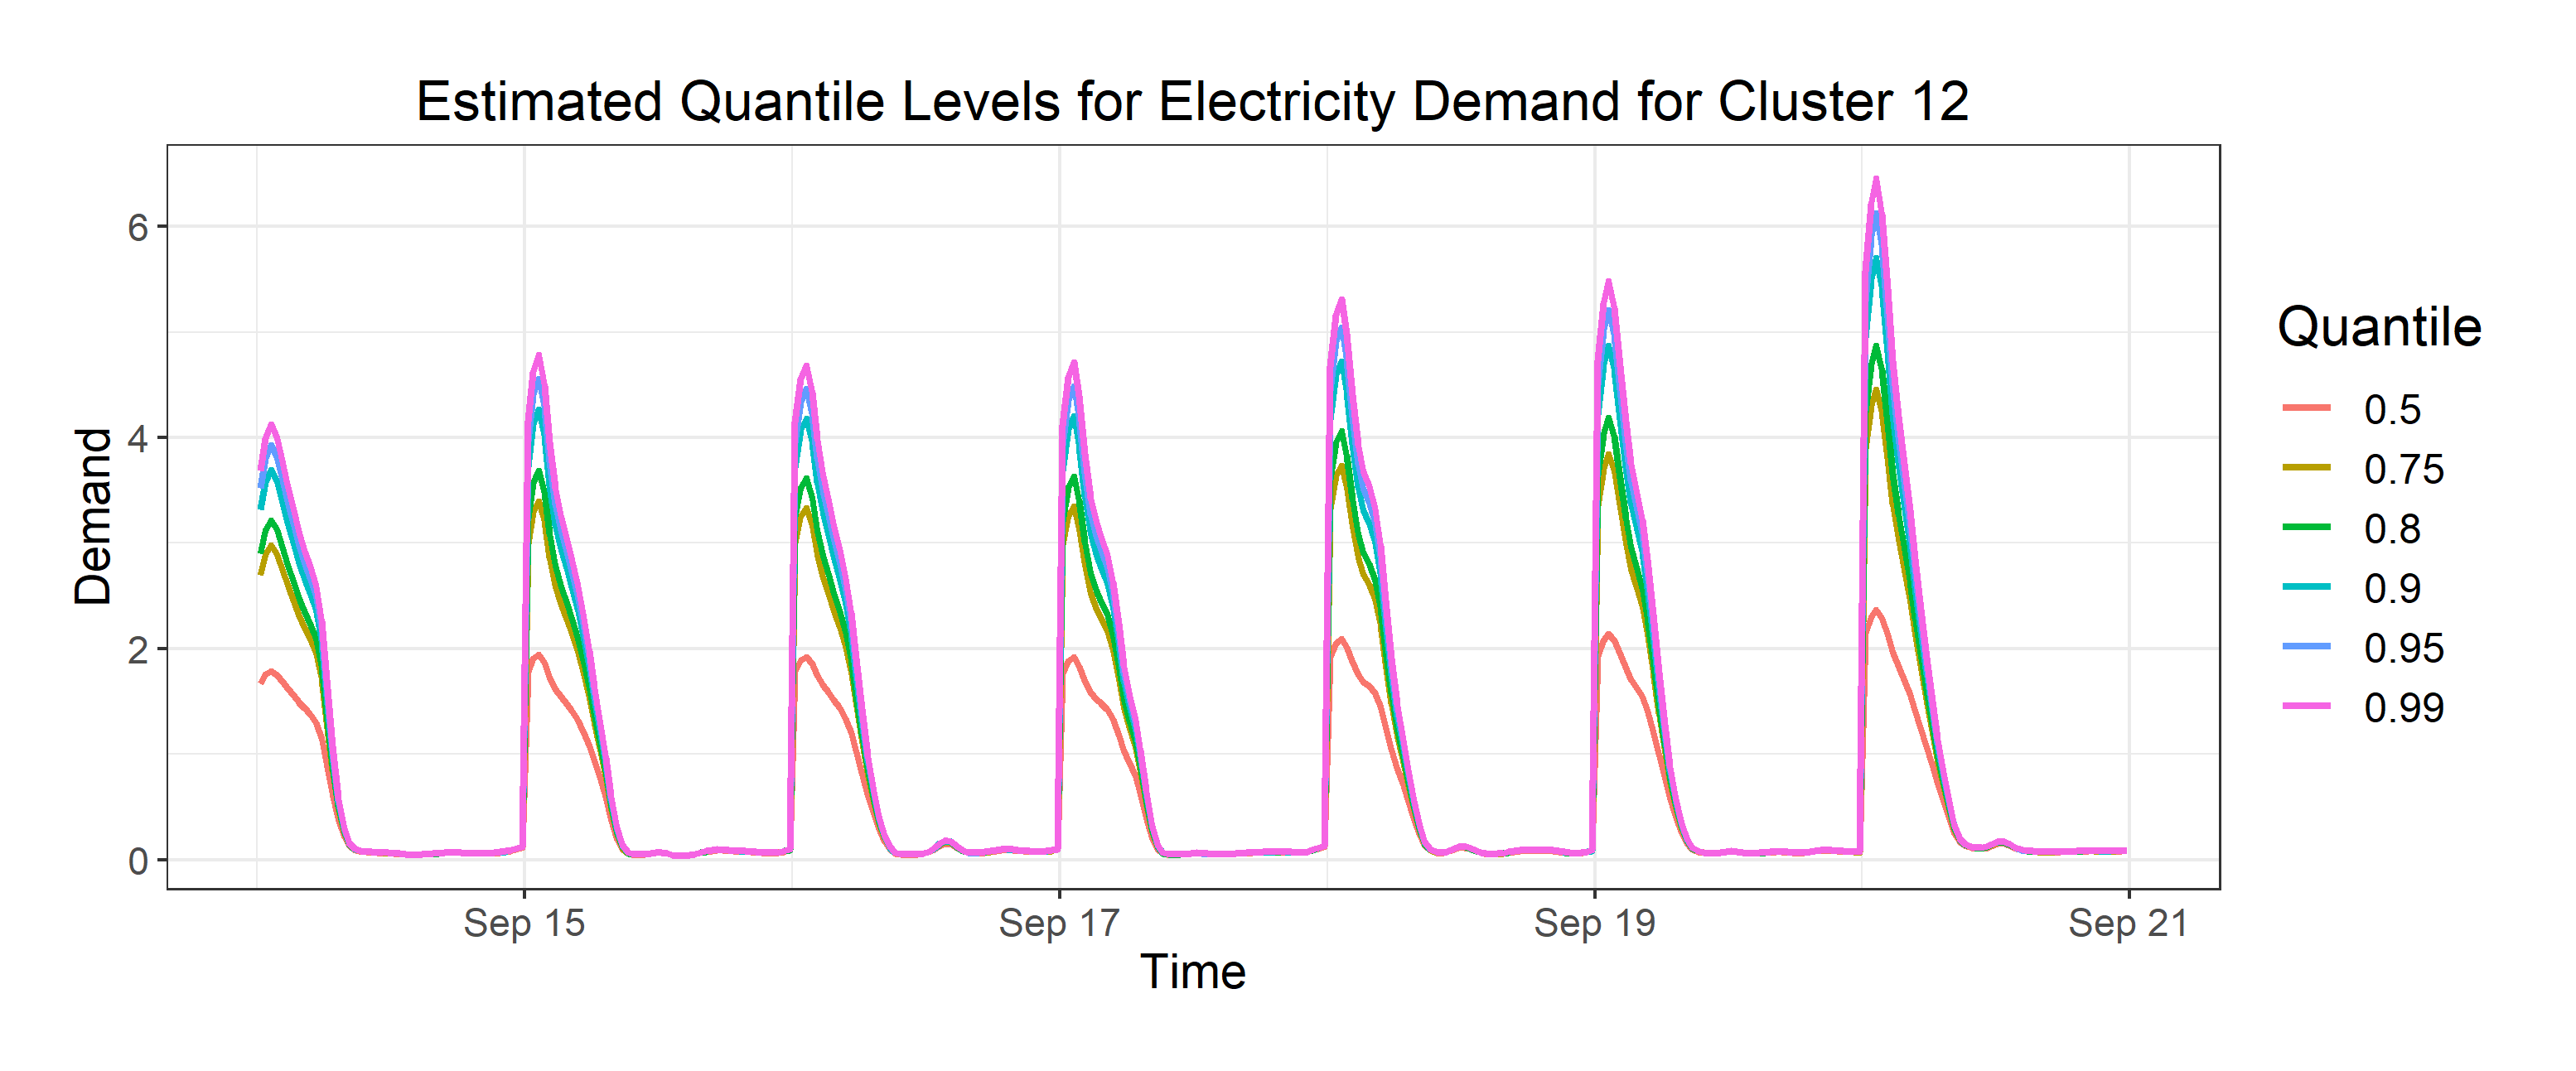
\includegraphics[width=\textwidth]{figures/quantlevel-12.png}
%      \end{subfigure}
%      \caption{Predicted quantile curves for Sept 14, 2015, to Sept 20, 2015, for different household clusters (Cluster 1 to 12)}
%      \label{fig:estimate-cluster}
% \end{figure}

\begin{figure}[!ht]
    \centering
    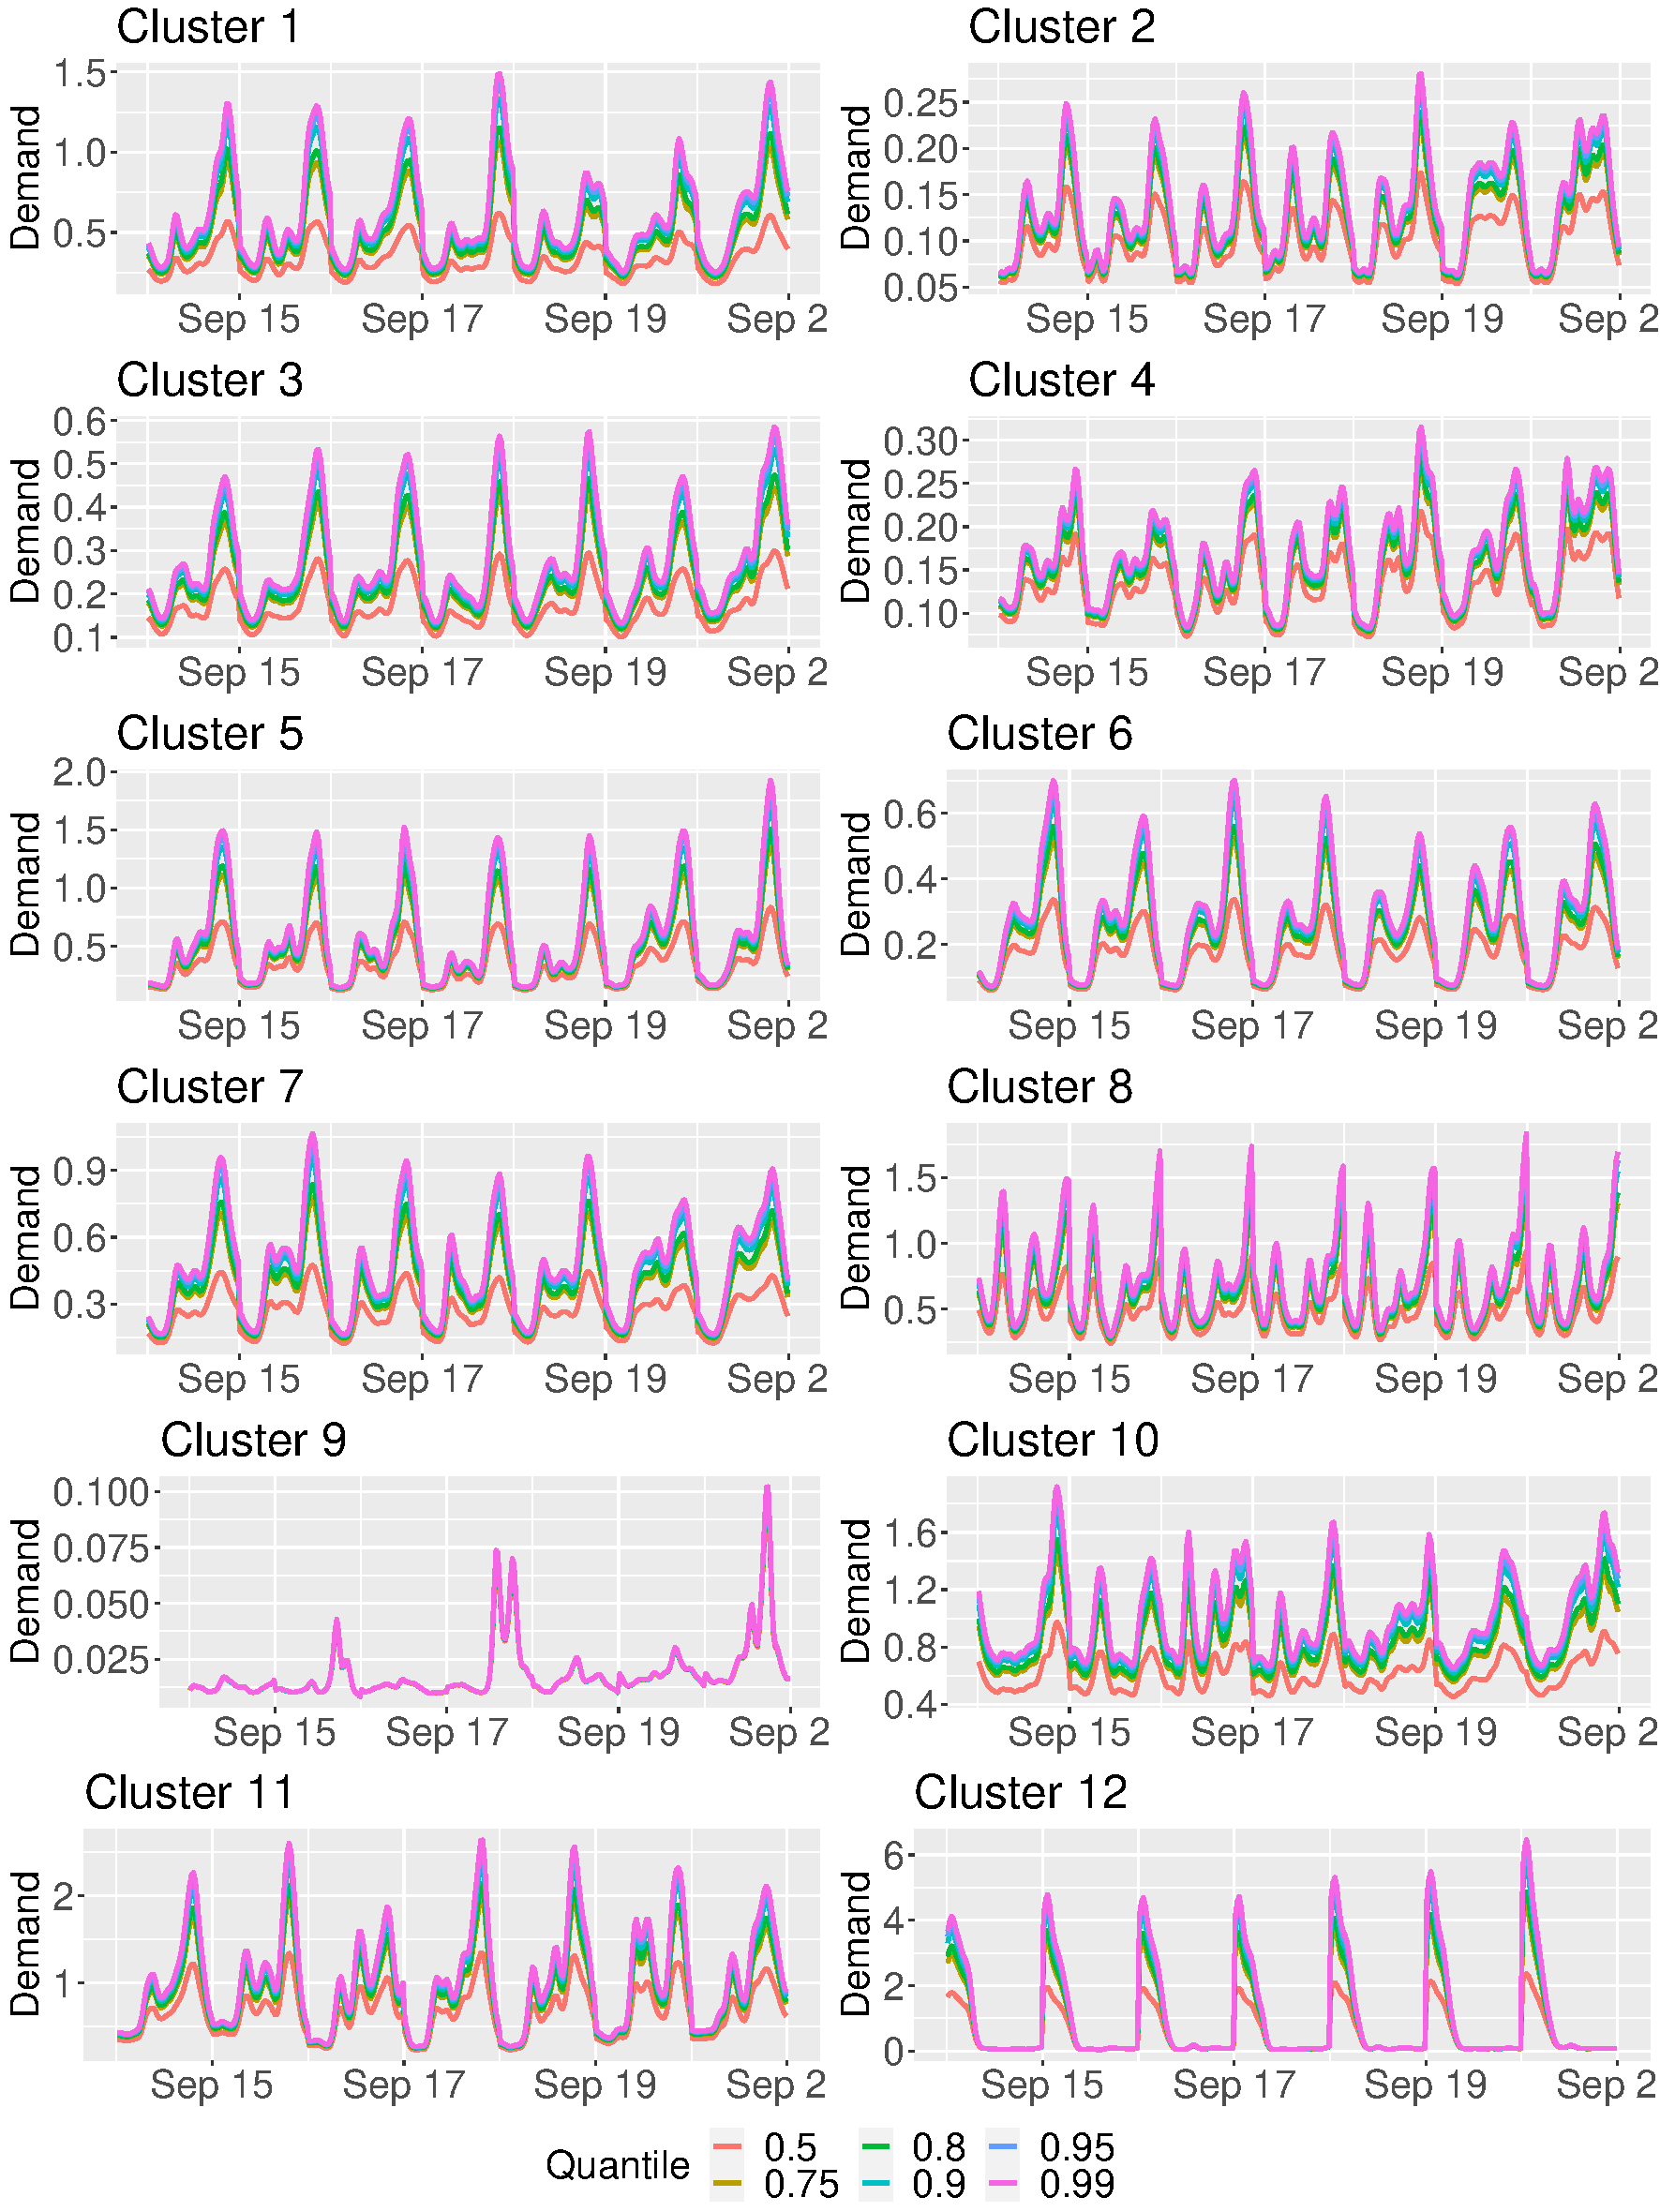
\includegraphics[width=0.9\textwidth,keepaspectratio]{prediction_plot.pdf}
    \caption{Predicted quantile curves for the demand during the last week of the dataset, for different households in the 12 clusters.}
    \label{fig:estimate-cluster}
\end{figure}

It is evident that the estimated quantile has a nice smoothness property due to the continuous and smooth nature of the kernel function, as well as it does not have any quantile crossing issue. As expected, the two quantile curves are closer when the general trend demand is low, but during the peak hours, the quantiles can become extremely different from the usual median trend level. The systematic cyclical pattern which is present in electricity demand due to the daily day-night cycle is also captured in the prediction. Some clusters like clusters 2, 4, 8 and 12 indicate high electricity loads during the weekends. While for most of the clusters, the quantile curves vary, the quantile curves for cluster 9 are very tightly packed together. This is because there are only two households, namely Household 106 and Household 207 lying in this cluster, making the number of spatial points insufficient to produce a reliable estimate of the variations in the quantile. Also, the pattern of the cyclical nature of the electricity demand for Cluster 12 is different from the other households, with the peak value occurring at the beginning of the day only. These correspond to Households 202, 210, and others.




%%%%%%%%%%%%%%%%%%%%%%%%%%%%%%%%%%%%%%%%%%%%%%%%%%%%%%%%%%%%%
%%                  The Bibliography                       %%
%%                                                         %%
%%  imsart-???.bst  will be used to                        %%
%%  create a .BBL file for submission.                     %%
%%                                                         %%
%%  Note that the displayed Bibliography will not          %%
%%  necessarily be rendered by Latex exactly as specified  %%
%%  in the online Instructions for Authors.                %%
%%                                                         %%
%%  MR numbers will be added by VTeX.                      %%
%%                                                         %%
%%  Use \cite{...} to cite references in text.             %%
%%                                                         %%
%%%%%%%%%%%%%%%%%%%%%%%%%%%%%%%%%%%%%%%%%%%%%%%%%%%%%%%%%%%%%
%
%% if your bibliography is in bibtex format, uncomment commands:
\bibliographystyle{imsart-nameyear.bst} % Style BST file (imsart-number.bst or imsart-nameyear.bst)
\bibliography{QRreferences.bib}      % Bibliography file (usually '*.bib')


\appendix

\section{Proof of Proposition~\ref{prop:P1P3}}\label{appA}

\subsection{Proof \cnam{of~}\ref{prop:first-div-dist}}\label{proof:first-div-dist}

\begin{multline*}
    -a_n \nabla \Mcal_{\bb{u},n}^{(p)}(\bb{q}_0)
    = \dfrac{a_n}{n} \sum_{i=1}^n \bb{K}(t_i) \left(\dfrac{\bb{\eta}(t_i)}{\Vert \bb{\eta}(t_i)\Vert} + \bb{u} \right) + \dfrac{a_n}{n} \sum_{i=1}^n \bb{K}(t_i) \bb{V}_2(t_i)\bb{V}_1^{1/2}(t_i) \bb{\xi}(t_i)\\
    + \dfrac{a_n}{n}\sum_{i=1}^n \mathcal{O}_p(\Vert \bb{K}(t_i) \Vert \Vert \bb{\eta}(t_i)\Vert^{-3} \Vert \bb{V}_1^{1/2}(t_i) \Vert \Vert \bb{\xi}(t_i) \Vert^2)
\end{multline*}
\noindent Let us start with the third term. Due to the sub-gaussian nature of $\bb{\xi}(t)$ for any $t \in \Tcal$, $\Vert \bb{\xi}(t) \Vert = \mathcal{O}_p(\sqrt{p})$, $\Vert \bb{\xi}(t) \Vert^2 = \mathcal{O}_p(p + \sqrt{p})$ and $\Vert \bb{\xi}(t)\Vert^3 = \mathcal{O}_p(p\sqrt{p} + p)$, with probability at least $(1 - e^{-Cp})$. Also, since each element of the kernel matrix is $\mathcal{O}(b_n)$, its norm is bounded by $\mathcal{O}(\sqrt{p}b_n)$ asymptotically almost surely~\citep{tao2012topics}. Therefore, it follows that
\begin{equation*}
    \dfrac{a_n}{n}\sum_{i=1}^n \mathcal{O}_p(\Vert \bb{K}(t_i) \Vert \Vert \bb{\eta}(t_i)\Vert^{-3} \Vert \bb{V}_1^{1/2}(t_i)\Vert \Vert \bb{\xi}(t_i) \Vert^2)
    = O\left( \dfrac{a_n b_n^2 p^{3/4} (p+\sqrt{p}) }{b_n^3 (p\sqrt{p} - p)^2 } \right) = O\left( b_n^{-2}p^{-9/4} \right).
\end{equation*}
\noindent Since $p^{9/8}b_n \rightarrow \infty$ as $n \rightarrow \infty$, it follows that this third term goes to $0$ asymptotically almost surely.

Turning to the first term, we note that $\left\Vert \dfrac{\bb{\eta}(t_i)}{\Vert \bb{\eta}(t_i)\Vert} \right\Vert \leq 1$ and $\Vert \bb{u} \Vert \leq 1$. Consequently, we can rewrite it as
\begin{align*}
    & \quad \dfrac{a_n}{n}\sum_{i=1}^n \bb{K}(t_i) \left(\dfrac{\bb{\eta}(t_i)}{\Vert \bb{\eta}(t_i)\Vert} + \bb{u} \right)\\
    = & \quad \dfrac{a_n}{n}\sum_{i=1}^n \bb{K}(t_i) \left( \dfrac{\bb{\eta}(t_i)}{\Vert \bb{\eta}(t_i)\Vert} - \E_{\bb{Y}(t) \mid \bb{X}(t) = \bb{x}}\left( \dfrac{\bb{Y}(t) - \bb{q}_0}{\Vert \bb{Y}(t) - \bb{q}_0 \Vert} \right) \right) + \\
    & \quad \quad \quad \dfrac{a_n}{n}\sum_{i=1}^n \bb{K}(t_i) \E_{\bb{Y}(t) \mid \bb{X}(t) = \bb{x}}\left( \dfrac{\bb{Y}(t) - \bb{q}_0}{\Vert \bb{Y}(t) - \bb{q}_0 \Vert} + \bb{u} \right)\\
    = & \quad \dfrac{a_n}{n}\sum_{i=1}^n \bb{K}(t_i) \left( \dfrac{\bb{\eta}(t_i)}{\Vert \bb{\eta}(t_i)\Vert} - \E_{\bb{Y}(t) \mid \bb{X}(t) = \bb{x}}\left( \dfrac{\bb{Y}(t) - \bb{q}_0}{\Vert \bb{Y}(t) - \bb{q}_0 \Vert} \right) \right), \\
    & \quad \quad \quad \text{as the second summand is equal to $0$ by Lemma~\ref{lemma:estimating-eqn}.}\\
    = & \quad \dfrac{a_n}{n}\sum_{i=1}^n \bb{K}(t_i) \left( \dfrac{\bb{\eta}(t_i)}{\Vert \bb{\eta}(t_i)\Vert} - \dfrac{\bb{\mu}(t) - \bb{q}_0}{\Vert \bb{\mu}(t) - \bb{q}_0 \Vert} + O\left( p^{-1/2} \right) \right)\\
    = & \quad \dfrac{a_n}{n}\sum_{i=1}^n \bb{K}(t_i) \left( \dfrac{\bb{\eta}(t_i)}{\Vert \bb{\eta}(t_i)\Vert} - \dfrac{\bb{\mu}(t) - \bb{q}_0}{\Vert \bb{\mu}(t) - \bb{q}_0 \Vert} \right) + \mathcal{O}(b_n^{-1}p^{-3/2})
\end{align*}
\noindent where we again apply Taylor series decomposition for $\E_{\bb{Y}(t) \mid \bb{X}(t) = \bb{x}}\left( \dfrac{\bb{Y}(t) - \bb{q}_0}{\Vert \bb{Y}(t) - \bb{q}_0 \Vert} \right)$ and bound the norms using standard sub-gaussian tail bounds. Clearly, as $b_n^{-2}p^{-9/4} \rightarrow 0$, it readily follows that $b_n^{-1}p^{-3/2} \rightarrow 0$ as $n \rightarrow \infty$. In view of \eqref{eqn:keydef-eta}, the first term here converges to $\bb{\eta}_t(\bb{q}_0)$ in the limit. 

We also note that the variance of $\sum_{i=1}^n \bb{K}(t_i) (\bb{\eta}(t_i)/\Vert \bb{\eta}(t_i)\Vert + \bb{u})$ is bounded through
\begin{multline*}
    \left\Vert \var\left( \dfrac{a_n}{n} \sum_{i=1}^n \bb{K}(t_i) \left( \dfrac{\bb{\eta}(t_i)}{\Vert \bb{\eta}(t_i) \Vert} + \bb{u}\right) \right) \right\Vert
    \leq \dfrac{a_n^2}{n^2} \sum_{i=1}^n \Vert \bb{K}(t_i)\Vert^2 \left\Vert \var\left( \dfrac{\bb{\eta}(t_i)}{\Vert \bb{\eta}(t_i) \Vert} \right) \right\Vert\\
    = O\left( \dfrac{a_n^2}{n} (p+\sqrt{p})b_n^2 \right)
    = O\left( (np)^{-1} \right)
\end{multline*}
\noindent where $\left\Vert \var\left( \bb{\eta}(t_i) / \Vert \bb{\eta}(t_i)\Vert \right) \right\Vert = \mathcal{O}(1)$ as the norm of the random variable is uniformly bounded by $1$. Clearly, as $n \rightarrow \infty$, the variance tends to $0$ \cnam{which, given the assumptions in the proposition, implies} 
\begin{equation*}
    \left\Vert \frac{a_n}{n} \sum_{i=1}^n \bb{K}(t_i) \left(\dfrac{\bb{\eta}(t_i)}{\Vert \bb{\eta}(t_i)\Vert} + \bb{u} \right) - \bb{\eta}_t(\bb{q}_0) \right\Vert \xrightarrow{P} 0.
\end{equation*}
%where $\bb{\eta}_t(\bb{q}_0)$ is a deterministic quantity described as in~\eqref{eqn:keydef-eta}.

Finally, we consider the second term. Note that, $\bb{\eta}(t_i)$, $\bb{V}_1(t_i)$ and $\bb{V}_2(t_i)$ are all predictable with respect to the filtration $\{ \mathcal{F}_{t} : t \in \Tcal \}$. Therefore, $\bb{K}(t_i)\bb{V}_2(t_i)\bb{V}_1^{1/2}(t_i)\bb{\xi}(t_i)$ is a martingale difference with respect to the same filtration. Letting $\bb{\zeta}(t_i) := \frac{a_n}{n} \bb{K}(t_i)\bb{V}_2(t_i)\bb{V}_1^{1/2}(t_i)\bb{\xi}(t_i)$, we obtain
\begin{equation*}
    \bb{\Sigma}_{\zeta, i}^2
    = \E\left[ \bb{\zeta}(t_i)\bb{\zeta}(t_i)\tr \mid \Fcal_{t_{i-1}} \right]
    = \frac{a_n^2}{n^2} \bb{K}(t_i) \bb{V}_2(t_i)\bb{V}_1(t_i)\bb{V}_2(t_i)\tr \bb{K}(t_i)
\end{equation*}
\noindent In view of \eqref{eqn:keydef-omega}, 
\begin{equation*}
    \Delta_n := \left\Vert \sum_{i=1}^n \bb{\Sigma}_{\zeta,i}^2 - \bb{\Omega}_t(\bb{q}_0) \right\Vert \rightarrow 0, \ \text{ as } n \rightarrow \infty.
\end{equation*}
\noindent Let, $f \in \mathcal{F}$, the set of three-times differentiable functions with bounded first, second and third derivative, and let $c_2$ and $c_3$ denote the upper bound of the second and third derivative of $f$ respectively.  Then, application of the quantitative central limit theorem for the multidimensional martingale~\citep{belloni2018high} ensures that
\begin{equation*}
    \left\Vert \E\left[ f\left(\dfrac{a_n}{n} \sum_{i=1}^n \bb{\zeta}(t_i) \right) \right] - \E \left[ f(\bb{Z}^{\ast}(\bb{q}_0)) \right] \right\Vert  \leq 2c_2 \Delta_n + c_3 \sum_{i=1}^n \E\left[ \left\Vert \bb{\zeta}(t_i) \right\Vert^3 \right],
\end{equation*}
where $\bb{Z}^\ast(\bb{q}_0)$ is a mean-zero Gaussian vector with dispersion matrix $\bb{\Omega}_t(\bb{q}_0)$. Since $\Delta_n \rightarrow 0$, then
\begin{equation*}
    \sum_{i=1}^n \E\left[ \left\Vert \bb{\zeta}(t_i) \right\Vert^3 \right]
    = \mathcal{O}\left(\dfrac{a_n^3}{n^3}\sum_{i=1}^n (p\sqrt{p}+p)^3 b_n^3 \right)
    = \mathcal{O}(n^{-2}p^{3/2}).
\end{equation*}
Additionally, it follows from $p^2/n \rightarrow 0$ that $n^{-2}p^{3/2} \rightarrow 0$, as $n \rightarrow \infty$.

Combining all these using Slutsky's theorem, we have for any fixed $\bb{u} \in B^{p-1}$ and for sufficiently large $n$,
\begin{equation*}
    \sup_{f \in \mathcal{F}} \left\Vert \E\left[f \left(a_n (\widehat{q}_n(\bb{u},\bb{x}) - Q(\bb{u},\bb{x}) \right)\right] - \E\left[ f\left( -\bb{\Omega}_t^{-1/2}(\bb{q}_0)\bb{Z}(\bb{q}_0) \right) \right] \right\Vert = \mathcal{O}\left(\max\{p^2/n, b_n^{-1}p^{-9/8}  \} \right)
\end{equation*}
\noindent \sredit{where  $\bb{Z}(\bb{q}_0)$ is given as in the statement of proposition~\ref{prop:first-div-dist}.} Finally, we can apply a standard $\epsilon$-net argument (see Section 2.3.1 of \cite{tao2012topics}) with union bounds over the unit ball $B^{p-1}$ to take a supremum over the choice of $\bb{u}$, which transforms the above into uniform convergence as needed in the proposition~\ref{prop:first-div-dist}.

\subsection{Proof of~\ref{prop:second-div-mat}}\label{proof:second-div-mat}

First, we express the term $\nabla^2 \Mcal_{\bb{u},n}^{(p)}(\bb{q})$ by computing the second order derivative of the objective function $\Mcal_{\bb{u},n}^{(p)}(\bb{q})$ as follows
\begin{equation*}
    \nabla^2 \Mcal_{\bb{u},n}^{(p)}(\bb{q}) 
    = \dfrac{1}{n}\sum_{i=1}^n \bb{K}(t_i) \left[ \dfrac{I_p}{\left\Vert  \bb{Y}(t_i) - \bb{q} \right\Vert_{\bb{K}(t_i)} } 
 - \dfrac{\bb{K}(t_i)(\bb{Y}(t_i) - \bb{q})(\bb{Y}(t_i) - \bb{q})\tr \bb{K}(t_i)}{\left\Vert  \bb{Y}(t_i) - \bb{q} \right\Vert^3_{\bb{K}(t_i)}} \right] \bb{K}(t_i).
\end{equation*}
\noindent We perform an M-R decomposition technique on $\nabla^2 \Mcal_{\bb{u},n}^{(p)}(\bb{q})$ as in~\cite{zhao2008confidence} and rewrite 
\begin{equation*}
    \nabla^2 \Mcal_{\bb{u},n}^{(p)}(\bb{q}) = M_{n,p} + R_{n,p}
\end{equation*}
\noindent where 
\begin{align*}
    \bb{a}(t_i) & = \bb{K}(t_i) (\bb{Y}(t_i) - \bb{q}),\\
    R_{n,p} & = \dfrac{1}{n}\sum_{i=1}^n \bb{K}(t_i) \E\left[ \dfrac{I_p}{\Vert \bb{a}(t_i)\Vert } - \dfrac{\bb{a}(t_i) \bb{a}(t_i)\tr}{\Vert \bb{a}(t_i)\Vert^3 }  \mid \Gcal_{t_i-1} \right] \bb{K}(t_i),\\
    M_{n,p} & = \dfrac{1}{n}\sum_{i=1}^n \bb{K}(t_i) \left[ \dfrac{I_p}{\Vert \bb{a}(t_i)\Vert } - \dfrac{\bb{a}(t_i) \bb{a}(t_i)\tr}{\Vert \bb{a}(t_i)\Vert^3 } \right] \bb{K}(t_i) - R_{n,p}.
\end{align*}
\noindent We note that $M_{n,p}$ is the partial average of a martingale difference sequence with respect to the filtration $\{ \Gcal_{t} : t \in \Tcal \}$. Applying the quantitative central limit theorem for multidimensional martingale~\citep{belloni2018high}, it follows that $M_{n,p} = \mathcal{O}(pb_n)$ which goes to $0$ as $n \rightarrow 0$. The conditions for applying the quantitative central limit theorem are similar to the ones shown in the appendix~\ref{proof:first-div-dist} and can be verified easily.

To deal with $R_{n,p}$, we expand $\bb{a}(t_i) = \bb{\eta}(t_i) + V_1^{1/2}(t_i) \bb{\xi}(t_i)$ and apply Taylor series expansion of the normalized errors about the origin. Hence,
\begin{equation*}
    R_{n,p} = \dfrac{1}{n}\sum_{i=1}^n \bb{K}(t_i) \left[ \dfrac{I_p}{\Vert \bb{\eta}(t_i)\Vert } - \dfrac{\bb{\eta}(t_i) \bb{\eta}(t_i)\tr}{\Vert \bb{\eta}(t_i)\Vert^3 } \right] \bb{K}(t_i) + \mathcal{O}(\sqrt{pb_n}),
\end{equation*}
where we use the fact that $\E\left[ \bb{\xi}(t_i) \mid \Gcal_{t_i-1} \right] = 0$ by independence of the errors and the filtration $\{ \Gcal_t : t\in \Tcal\}$ and mean-zero property of the errors. Note that, the matrix 
\begin{equation*}
    \Vert \bb{\eta}(t_i) \Vert^2 I_p - \bb{\eta}(t_i)\bb{\eta}(t_i)\tr
\end{equation*}
\noindent is positive definite for all $n, p$ and $\bb{q} \notin \{\bb{Y}(t_i) : t_i \in \Tcal_n \}$. Therefore,
\begin{equation*}
    \left\Vert \nabla^2 \Mcal_{\bb{u},n}^{(p)}(\bb{q}) - \bb{\Psi}_t(\bb{q}_0) \right\Vert = O\left(pb_n, \sqrt{pb_n} \right),
\end{equation*}
and the precise result in~\ref{prop:second-div-mat} follows readily since $pb_n \rightarrow 0$ as $n\rightarrow 0$.



%===================================================

\section{Simulation study}
\label{Sec:simulation}

In this section, we focus on the finite-sample performance of the proposed spatio-temporal quantile estimation methodology in two distinct simulation frameworks. The first takes place in a full-fledged spatio-temporal setting, where the locations are treated in terms of a multivariate time series framework, without explicitly incorporating information on the spatial coordinates. In contrast, the second case has been designed so as to draw on the inter-connectedness of spatial coordinates to emulate typical features in spatio-temporal data. Both setting were chosen upon careful consideration for illustrating the overall potential and efficacy of the proposed nonparametric quantile estimation as part of this paper. In this exercise, in order to evaluate efficiency, we use two popular metrics -- thee mean absolute error (MAE) and the mean absolute percentage error (MAPE). 


\subsection{Simulation setup 1}

We use $p$ to denote the number of spatial points, and let $s_1,\hdots,s_p$ denote the positions of these points. In this setting, we assume that the exact coordinates of the locations are unknown. Therefore, to simplify the computations, we consider a regular set of the form $\{1,2,\hdots,p\}$ to denote the set of the spatial points. Throughout this experiment, the number of time points is fixed at $T=300$. The covariate series $\{\bb{X}(t)\}_{1\leqslant t\leqslant T}$ is assumed to be bivariate and we simulate it following a vector-valued autoregressive (VAR) series of order 1. In particular, $\bb{X}(t)$ is assumed to follows VAR(1) process with mean $\bb{0}$, satisfying the equation
\begin{equation*}
        \bb{X}(t) = \begin{bmatrix}
          0.2 & 0.1\\
          -0.3 & 0.4
        \end{bmatrix}
        \bb{X}(t-1) + \begin{bmatrix}
          w_{1t}\\
          w_{2t}
        \end{bmatrix},
\end{equation*}
where $w_{1t}, w_{2t}$ are uncorrelated white noise process. We shall use $\bb{X}_1(t)$ and $\bb{X}_2(t)$ to denote the two coordinates of the vector.
    
Next, the mean function associated with the response variable $\bb{Y}(t)$ (see \eqref{eqn:setup} for reference) is assumed to take the form
\begin{equation*}
        \bb{\mu}(\bb{X}(t)) = \begin{bmatrix}
          \alpha_1 + \beta_{1,1} t + \beta_{2,1}\sin(2\pi \bb{X}_1(t)) + \beta_{3,1}\cos(2\pi \bb{X}_2(t)) \\
          \alpha_2 + \beta_{1,2} t + \beta_{2,2}\sin(2\pi \bb{X}_1(t)) + \beta_{3,2}\cos(2\pi \bb{X}_2(t)) \\
          \vdots \\
          \alpha_p + \beta_{1,p} t + \beta_{2,p}\sin(2\pi \bb{X}_1(t)) + \beta_{3,p}\cos(2\pi \bb{X}_2(t))
    \end{bmatrix}.
\end{equation*}
\noindent Note that the above is a nonlinear function in $\bb{X}(t)$, and this formulation is useful to understand if the specified nonparametric method is effective in a general scenario. To generate the intercept terms ($\alpha_i$) in the above expression, for $i = 1, 2, \dots, p$, we use the standard normal distribution. The $\beta_{1,i}$ coefficients indicate a linear trend pattern, and they are generated independently from uniform distribution between $-1$ and $1$. Finally, the parameters $\beta_{2,i}$ and $\beta_{3,i}$, for all $i$, are obtained independently from a uniform distribution in the interval $(-20, 20)$. Note that these choices ensure a greater degree of dependence on $\bb{X}(t)$, and are helpful to assess the accuracy of the proposed technique. 

For the covariance structure in the model \eqref{eqn:setup}, we consider  
\begin{equation*}
    \bb{\Sigma}(\bb{X}(t)) = 0.1 \left\| \mu(\bb{X}(t))\right\| \begin{bmatrix}
        \exp\{-0.1(s - s\dash)^2\}
    \end{bmatrix}_{s, s\dash = 1}^p,
\end{equation*}
the second term indicating a matrix with $(s,s')^{th}$ element given by the exponentially decaying covariance function. We point out that this specification maintains the signal to the noise ratio close to $0.1$ throughout the process.

Based on the above simulation setup, we generate $B = 1000$ datasets, each with $300$ time-points and $10$ spatial coordinates. Then, using Monte Carlo simulation, we can approximate the expectation in \eqref{eqn:parameter} for any choice of $\bb{x}$ and $\bb{u}$, and, therefore, are able to optimize the objective function given in \eqref{eqn:parameter} to obtain $Q(\bb{u} ,\bb{x})$. To assess the accuracy of the proposed technique, we consider this value as the true quantile which we wish to estimate. Now, we randomly choose $100$ datasets among those $1000$, and for each of them, we compute the proposed estimator $\hat{q}(\bb{u} ,\bb{x})$ as in \eqref{eqn:estimator}. The errors are computed according to different sizes of the dataset, in terms of the number of time-points. Corresponding RMSE and MAPE values are summarized in \Cref{tab:sim-S1-RMSE}. Here, we choose a Gaussian kernel over the temporal and spatial domain, and restrict our attention to the choice of $\bb{u}$ as $(2\alpha - 1)\bb{1}_p/\sqrt{p}$, where $0 < \alpha < 1$ is the quantile of interest.

\begin{table}[ht]
\centering
\caption{MAE (MAPE given in parentheses) in estimating the $\bb{u}$-quantile at different time-points ($t$), where $\bb{u}=(2\alpha - 1)\bb{1}_p/\sqrt{p}$, under simulation setup 1.}
\label{tab:sim-S1-RMSE}
\begin{tabular}{cccccc}
  \toprule
 $\alpha$ & $t=10$ & $t=50$ & $t=150$ & $t=250$ & $t=290$ \\ 
  \midrule
  0.50 & 3.93 (10.75) & 0.69 (3.72) & 1.23 (4.04)  & 2.46 (3.42) & 3.65 (1.24) \\ 
  0.75 & 5.16 (15.97) & 2.12 (4.29) & 1.39 (5.17) & 3.72 (2.71) & 4.21 (1.87) \\ 
  0.80 & 5.26 (20.44) & 2.24 (4.58) & 1.46 (5.20) & 4.07 (2.61) & 4.36 (2.07) \\ 
  0.85 & 5.50 (22.96) & 2.50 (5.12) & 1.63 (5.35) & 4.09 (2.52) & 5.20 (2.45) \\ 
  0.90 & 7.83 (25.44) & 3.07 (9.03) & 2.91 (6.89) & 4.78 (2.97) & 6.56 (3.37) \\ 
   0.95 & 14.22 (27.87) & 3.23 (12.89) & 4.32 (10.70) & 6.50 (4.09) & 9.91 (4.86) \\ 
   \bottomrule
\end{tabular}
\end{table}

From the above table, we can observe that the percentage errors reduce substantially for larger sizes of the dataset. In estimating the median ($\alpha=0.5$), our proposed method makes only about 1.2\% error if 290 observations per time series are allowed. The MAPE typically remains less than 3\% for moderate quantiles, and for more than 250 observations per spatial point. The errors are slightly higher for more extreme quantiles. For instance, at $\alpha=0.95$ and for $t\geqslant 250$, our technique incurs 4 to 5 percent error on average. 

In order to demonstrate the predictive performance of the method, we use the observations for $t\leqslant 290$ as the training set, and then forecast the quantiles for the next time-points. The RMSE and MAPE thus computed, across 100 different datasets, are reported in \Cref{tab:sim-S1-pred-RMSE}. We can see that the errors vary between 3\% to 9.2\%, and stays around 4 to 5 percent in most of the cases. The method is robust in predicting 1 to 5 steps ahead. For different quantiles though, we see slightly different behaviors. For central quantiles, typically the errors are more, whereas for the extreme quantiles, our approach registers better accuracy with the MAPE of around 3 to 4.5 percent.

\begin{table}[ht]
\centering
\caption{MAE (MAPE given in parentheses) in predicting the $\bb{u}$-quantile, where $\bb{u}=(2\alpha - 1)\bb{1}_p/\sqrt{p}$, for simulation setup 1.}
\label{tab:sim-S1-pred-RMSE}
\begin{tabular}{cccccc}
  \toprule
   $\alpha$ & $1$-step ahead & $2$-step ahead & $3$-step ahead & $4$-step ahead & $5$-step ahead \\ 
  \midrule
   0.50 & 11.653 (6.361) & 11.876 (6.496) & 9.305 (4.997) & 16.723 (9.18) & 9.57 (5.16) \\ 
   0.75 & 10.686 (5.776) & 10.496 (5.666) & 7.003 (3.693) & 14.093 (7.704) & 7.489 (3.999) \\ 
   0.80 & 10.129 (5.478) & 9.882 (5.318) & 6.473 (3.4) & 13.413 (7.322) & 7.012 (3.736) \\ 
   0.85 & 10.689 (5.839) & 9.342 (5.048) & 5.879 (3.076) & 12.588 (6.857) & 6.481 (3.449) \\ 
   0.90 & 9.847 (5.362) & 9.722 (5.287) & 6.009 (3.184) & 11.527 (6.261) & 5.835 (3.108) \\ 
   0.95 & 8.735 (4.666) & 8.166 (4.387) & 5.493 (2.876) & 11.629 (6.331) & 5.855 (3.095) \\ 
   \bottomrule
\end{tabular}
\end{table}

\subsection{Simulation setup 2}

In the second simulation scenario, unlike the previous multivariate setup where only partial spatial information is assumed to be known, we focus on a spatio-temporal framework to generate the data where the actual spatial information is used in an explicit manner. We follow the work of \cite{das2017analyzing}, where the authors considered the spatio-temporal estimation problem from a Bayesian paradigm.  

To develop this model, $p=15$ spatial locations $\bb{s}_1, \dots \bb{s}_{15}$ are first generated uniformly in the unit square $[0, 1]$. Thus, $\Scal_p = \{ \bb{s}_1, \dots \bb{s}_{15}\}$, and $\bb{s}_i = (s_{i1}, s_{i2})$ with $0 \leqslant s_{i1}, s_{i2} \leqslant 1$. Next, we take $200$ equidistant points in the interval $[0, 1]$ as the time-points. In other words, $\Tcal_n = \{ t_1, t_2, \dots t_n \}$ with $t_1 = 0, t_n = 1$ and $(t_i - t_{i-1}) = 1/(n-1)$ for all $i = 2, \dots n$.
    
We now assume that $\bb{X}(t) = t$ for all $t \in \Tcal = [0, 1]$. This can be construed as a linear trend function. The conditional quantile-curve of level $\tau \in [0, 1]$, conditioned on the temporal variable $t$ and spatial variable $\bb{s}$, takes the form
\begin{equation}\label{eqn:quantile-curve-setup2}
    Q(\tau \mid t, \bb{s}) = t \xi_1(\tau, \bb{s}) + (1-t) \xi_2(\tau, \bb{s}),
\end{equation}
so that
\begin{equation*}
    \xi_1(\tau, \bb{s}_i) = \left( 1 - \dfrac{s_{i1} + s_{i2}}{2} \right)\tau^2 + s_{i1} \dfrac{\log(1+\tau)}{2\log 2} + \dfrac{s_{i2}}{2}\tau^3
\end{equation*}
and
\begin{equation*}
    \xi_2(\tau, \bb{s}_i) = (1 - s_{i2}^2)\sin\left(\tau \pi /2 \right) + s_{i2} \dfrac{(e^{\tau} - 1)}{(e - 1)}.
\end{equation*}


Owing to the inverse relationship between the quantile and the distribution function, we can generate observations from the above model by simulating uniform $[0, 1]$ random variables and evaluating the quantile function at those generated values. More relevant details of this approach can be found in~\cite{das2017analyzing}.

\begin{table}[ht]
\centering
\caption{MAE (MAPE given in parentheses) in estimating the $\tau$-quantile at different time-points ($t$) under simulation setup 2.}
\label{tab:sim-S2-MAE}
\begin{tabular}{cccccc}
  \toprule
  $\tau$ & $t = 0$ & $t = 0.25$ & $t = 0.5$ & $t = 0.75$ & $t = 1$ \\ 
  \midrule
  0.50 &  0.129 (1.44) & 0.037 (0.47) & 0.019 (0.27) & 0.119 (2.07) & 0.388 (8.28) \\ 
  0.75 & 0.135 (1.51) & 0.033 (0.42) & 0.045 (0.66) & 0.211 (3.67) & 0.547 (11.66) \\ 
  0.8 & 0.155 (1.73) & 0.035 (0.44) & 0.056 (0.82) & 0.238 (4.14) & 0.587 (12.51) \\ 
  0.85 & 0.171 (1.92) & 0.037 (0.47) & 0.068 (1) & 0.263 (4.58) & 0.629 (13.4) \\ 
  0.9 & 0.185 (2.08) & 0.037 (0.48) & 0.08 (1.18) & 0.291 (5.06) & 0.67 (14.29) \\ 
  0.95 & 0.205 (2.29) & 0.042 (0.54) & 0.096 (1.42) & 0.323 (5.62) & 0.721 (15.37) \\ 
  0.99 & 0.314 (3.52) & 0.082 (1.05) & 0.111 (1.63) & 0.348 (6.06) & 0.758 (16.16) \\
   \bottomrule
\end{tabular}
\end{table}


\begin{table}[ht]
\centering
\caption{MAE (MAPE given in parentheses) in estimating the $\tau$-quantile at different time-points ($t$) under simulation setup 2 with $90$ time-points and $10$ locations in training set.}
\label{tab:sim-S2-MAE-pred}
\begin{tabular}{rlllll}
  \hline
 $\tau$ & $t = 0.91$ & $t = 0.92$ & $t = 0.93$ & $t = 0.94$ & $t = 0.95$ \\ 
  \hline
    0.5 & 0.343 (6.64) & 0.355 (6.93) & 0.367 (7.23) & 0.38 (7.54) & 0.393 (7.86)  \\ 
  0.75 & 0.158 (1.7) & 0.152 (1.64) & 0.146 (1.58) & 0.14 (1.52) & 0.134 (1.46)  \\ 
  0.8 & 0.352 (3.41) & 0.343 (3.34) & 0.335 (3.26) & 0.326 (3.19) & 0.318 (3.11)  \\ 
  0.85 & 0.695 (6.1) & 0.685 (6.03) & 0.675 (5.95) & 0.664 (5.87) & 0.654 (5.8) \\ 
  0.9 & 1.214 (9.69) & 1.204 (9.63) & 1.194 (9.56) & 1.184 (9.5) & 1.174 (9.43) \\ 
  0.95 & 1.922 (14.01) & 1.916 (13.97) & 1.909 (13.93) & 1.902 (13.89) & 1.896 (13.85) \\ 
  0.99 & 2.601 (17.65) & 2.599 (17.64) & 2.597 (17.63) & 2.596 (17.62) & 2.594 (17.61)  \\ 
  & & & & & \\
   \hline
   $\tau$ & $t = 0.96$ & $t = 0.97$ & $t = 0.98$ & $t = 0.99$ & $t = 1$ \\ 
  \hline
    0.5 & 0.406 (8.19) & 0.419 (8.53) & 0.433 (8.89) & 0.447 (9.25) & 0.461 (9.63) \\ 
  0.75 &  0.128 (1.4) & 0.123 (1.35) & 0.117 (1.29) & 0.112 (1.24) & 0.107 (1.19) \\ 
  0.8 &  0.309 (3.04) & 0.301 (2.97) & 0.293 (2.9) & 0.285 (2.83) & 0.277 (2.76) \\ 
  0.85 &  0.644 (5.72) & 0.634 (5.64) & 0.625 (5.57) & 0.615 (5.49) & 0.605 (5.42) \\ 
  0.9 &  1.164 (9.36) & 1.155 (9.3) & 1.145 (9.23) & 1.135 (9.17) & 1.126 (9.11) \\ 
  0.95 &  1.889 (13.81) & 1.882 (13.77) & 1.876 (13.73) & 1.869 (13.7) & 1.863 (13.66) \\ 
  0.99 &  2.593 (17.6) & 2.591 (17.59) & 2.589 (17.58) & 2.588 (17.58) & 2.586 (17.57) \\ 
  \hline
\end{tabular}
\end{table}

We have generated 100 datasets aimed at illustrating the finite sample behaviour of the quantile function for the above case. Then, the accuracy of the model is computed by checking the errors of these estimates with respect to the true quantile given by~\eqref{eqn:quantile-curve-setup2}. In \cref{tab:sim-S2-MAE}, we demonstrate the mean absolute errors (MAE) between the true quantile values and the fitted quantiles. The mean absolute percentage error (MAPE) is shown in the brackets. Clearly, the maximum error is merely $16\%$ in case of extreme quantiles, for the quantiles closer to the median the error is less than $5\%$. Also, as expected, the errors tend to increase as we move towards the extreme quantile or the right hand of the temporal domain due to the boundary effects.

We repeat the simulation exercise to measure the predictive performance of our proposed estimator as well. In this case, we use the first $90$ temporal points and $12$ locations as the training data, and use that to predict the behaviour of the quantiles for the rest of the $3$ locations for time-points $t = 0.91$ to $t = 1$. The summary measures MAE and MAPE are presented in \cref{tab:sim-S2-MAE-pred}. It highlights that the error increases slowly for multiple step ahead predictions, the percentage error in prediction is $17.5\%$ for extreme quantiles.



%\srcomment{Will add prediction RMSE (with less location / less time point)}. 

%\sd{Discuss the findings of the estimation/prediction accuracy. Then, provide a comparative outline of what we learnt from the two different setups.}

The first simulation setup imitates the data generating mechanism presented in this paper. Thus, the results present in simulation setup 1 corroborate our theoretical findings. On the other hand, simulation setup 2 describes the data generation mechanism through the specification of the quantile function. Therefore, the generated data may not satisfy the model~\eqref{eqn:setup}. Since, this particular simulation illustrates actual spatio-temporal data, it is important to verify if the proposed estimator works equally well under this setup. The aforementioned simulation illustrates this point. Due to the violation of these model assumptions, the errors in simulation setup 2 are more than the errors for setup 1, though the percentage error remains at an acceptable level for non-extreme quantiles.



\end{document}

